%%%%%%%%%%%%%%%%%%%%%%%%%%% mainthesis.tex %%%%%%%%%%%%%%%%%%%%%%%%%%%
% Template for University of Maryland Thesis and Dissertation files  %
% Written by   Michael Jarret                                        %
%              Joint Center for Quantum Information and Comp. Sci.   %
%              Department of Physics                                 %
%              University of Maryland, College Park                  %
%              June 1, 2016                                          %
% Modified: February 23, 2016 by Michael Jarret                      %
% Based upon: UMD Dissertation Template by Dorothea F Brosius        %
%             Institute for Electronics and Applied Physics          %
%             University of Maryland, College Park                   %
%             Version from June 2015                                 %
%%%%%%%%%%%%%%%%%%%%%%%%%%%%%%%%%%%%%%%%%%%%%%%%%%%%%%%%%%%%%%%%%%%%%%

\documentclass[letterpaper,12pt]{umd-thesis}  
\usepackage{mathptmx} % This is a close match to Times New Roman, which is recommended by the grad school

\usepackage{hyperref,xcolor} % This adds hyperlinks and allows you to choose the colors simply
\usepackage{graphicx,epstopdf}			
\graphicspath{{graphics/}} % This creates a graphics directory located at ./graphics
\usepackage{amsmath,amsthm,amsfonts,amssymb,mathrsfs,dsfont,breqn} % These are math packages
\usepackage{cleveref}  % Cleveref MUST come after ams packages if AMS packages are used.
\usepackage[numbers,sort&compress]{natbib}							% This is probably the most elegant citation package for the dissertation, but 																				others can be used.

%\includeonly{introduction,spectral-theory,optimization,1dgap,mocbound}

% These are my own custom latex commands, you uncomment if unwanted
\usepackage{lipsum} % This is for testing.
\usepackage{stmaryrd}
\usepackage{thmtools}
\usepackage{thm-restate}
\usepackage{bbm}

\makeatletter  % Allow the use of @ in command names
\long\def\@makecaption#1#2{%
  \vskip\abovecaptionskip
  \sbox\@tempboxa{{\captionfonts #1: #2}}%
  \ifdim \wd\@tempboxa >\hsize
    {\captionfonts #1: #2\par}
  \else
    \hbox to\hsize{\hfil\box\@tempboxa\hfil}%
  \fi
  \vskip\belowcaptionskip}
\makeatother   % Cancel the effect of \makeatletter

\newcommand{\Frac}[2]{\frac{\displaystyle #1}{\displaystyle #2}}
\newcommand{\vol}{\text{vol}}
\newcommand{\expected}[1]{\left \langle #1 \right \rangle}


\newtheorem{thm}{Theorem}
\newtheorem{lem}{Lemma}
\newtheorem{cor}{Corollary}
\newtheorem*{remark}{Remark}
\newtheorem{definition}{Definition}
\crefname{lem}{lemma}{lemmas}
\Crefname{lem}{Lemma}{Lemmas}
\crefname{thm}{theorem}{theorems}
\Crefname{thm}{Theorem}{Theorems}


\newcommand{\braket}[2]{\langle #1|#2\rangle}
\newcommand{\bra}[1]{\langle #1|}
\newcommand{\ket}[1]{|#1\rangle}
\newcommand{\Bra}[1]{\left<#1\right|}%for big ones
\newcommand{\Ket}[1]{\left|#1\right>}%for big ones
\newcommand{\Braket}[2]{\left< #1 \right| #2 \right>}
\renewcommand{\th}{^\mathrm{th}}
\newcommand{\tr}{\mathrm{Tr}}
\newcommand{\id}{\mathds{1}}
% Different font in captions
\newcommand{\captionfonts}{\small}



% Custom formatting options
\hypersetup{linktocpage, linkbordercolor=blue}  % Blue outlined hyperlinks in TOC

\numberwithin{equation}{chapter}  % This changes the numbering style to chapter.equation 
\numberwithin{thm}{chapter}
\numberwithin{lem}{chapter}
\numberwithin{cor}{chapter}
\numberwithin{definition}{chapter}

\bibliographystyle{plain}

\title{Spectral graph theory with applications to quantum adiabatic optimization} % Dissertation Title
\author{Michael Jarret Baume} % Name as it appears on university records
\department{Department of Physics}
\gradyear{2016} % Year of graduation
\degree{Doctor of Philosophy} % Your degree
\principaladvisor{Professor Stephen P. Jordan}[University of Maryland Institute for Advanced Computer Studies] % Your {advisor}[his department][his institution]
\coadvisor{Professor Alexey Gorshkov}[Department of Physics]% Comment out if no coadvisor

% Add any additional committee members in alphabetical order below. Each accepts the format:
% \reader{Name}[Department][Institution]. They will not be automatically ordered, so they must be
% entered alphabetically. Currently, Department and Institution aren't implemented.
\secondreader{Professor Jay Deep Sau}
\thirdreader{Professor Jeffrey Bub}[Department of Philosophy]
%\fourthreader{Reader Four}
%\fifthreader{Reader Five}
%\sixthreader{Reader Six}

% Uncomment the following line if someone other than your advisor or your co-advisor is your chair and add his/her details
\committeechair{Professor Andrew Childs}[Department of Computer Science]

% The options below should be self explanatory
% \coadvisorischair % Only use this if you did not add a committe chair
% \copyrightfalse
% \tablespagefalse
% \figurespagefalse
% \contentspagefalse
% \bibpagefalse

\begin{document}

% Type the abstract below
\begin{abstract}
    \lipsum[1]
%    \lipsum[2]
%    \lipsum[3]
\end{abstract} 

% This is the frontmater and can include the preface, foreword, dedication, and acknowledgements. Any
% of these can be commented out if unwanted.
\begin{preliminary}

%	\begin{preface}
%		\lipsum[4]
%	\end{preface}
	
%	\begin{foreword}
%		\lipsum[5]
%	\end{foreword}

	\begin{dedication}
		To the ignorance of youth, without which this never would have happened.
	\end{dedication}

	\begin{acknowledgements}
		It is nearly impossible to thank everyone that had a hand in my successful completion of this dissertation. Some of the people mentioned below are likely to not remember their relevance towards my progress, however their impact was substantial and will not be forgotten.
		
		This work would have been impossible without funding from Booz Allen Hamilton, The University of Maryland Department of Physics, Joint Quantum Institute (JQI), and Joint Center for Quantum Information and Computer Science (QuICS). I would like to thank each of them for their support. 
		
		First and foremost, I would like to thank my advisor Stephen P. Jordan. Stephen has been a wonderful mentor, collaborator, and friend, and I am quite proud of the work we have done together. I would also like to thank Jeffrey Bub, both for always providing much needed direction and advice. My path throughout graduate school has been far from traditional, and I ultimately found my way due to a path of advice and introductions that came from Diane O'Leary, Konstantina Trivisa, Eileen Zagone. Without these people, I surely would never have gotten to where I am.
		
		I would also like to thank the close friends who were with me through this period of my life. Above all else, I owe special thanks to Prabal Adhikari, my earliest and closest friend from the University of Maryland. Also always there to help me were Prabin Adhikari and Clare Scott. 
		
		My family: my mother, stepfather, and Uncle. (Uncle being capitalized because, in his case, it is a proper noun.) This dissertation should really be dedicated to them, however I would never let sentimentality inhibit humor. Last, I would like to thank my dog Matoskah (`Matty'), who constantly reminds me that there are more important things than work, such as throwing the ball.
	\end{acknowledgements}
% if you need a "List of Symbols or Abbreviations" look into
% gatech-thesis-gloss.sty.
\end{preliminary}

\let\oldrVert\rVert
\let\oldlVert\lVert

\renewcommand{\lVert}{\left\oldlVert}
\renewcommand{\rVert}{\right\oldrVert}

\chapter{Introduction}

This dissertation focuses on the problem of bounding the spectral gap of Schr\"{o}dinger operators. Although of reasonably broad mathematical interest, our primary motivation for studying this problem arises in the context of adiabatic quantum computing. Roughly speaking, adiabatic quantum algorithms slowly vary a quantum state that is easy to prepare into one that encodes the solution to some computational problem \cite{Farhi_science}. Although adiabatic quantum computation can perform universal quantum computation \cite{ADKLLR07}, the technique is most easily applied to optimization problems, our current focus. Quantum adiabatic theorems tell us precisely how slowly our variation must progress.

The dynamics of an adiabatic process, and of course all quantum processes, are governed by Schr\"{o}dinger's equation, $i \partial_t \psi(t) = H(t) \psi(t)$. The Hermitian operator $H$ is known as the Hamiltonian of the system, and we denote its spectrum $\lambda_0 \leq \lambda_1 \leq \lambda_2 \dots \leq \lambda_N$.\footnote{In general, these Hermitian operators $H$ are known as either Hamiltonians or Schr\"{o}dinger operators, where the term ``Schr\"{o}dinger operator'' is preferred in the differential equations literature, seemingly because of increased generality. Although ``Hamiltonian'' might imply something physical about the operator, in this dissertation we will use the two terms synonymously, as we are predominantly concerned with the mathematical properties of such operators.} We call $\gamma(s) = \lambda_1(s) - \lambda_0(s)$ the spectral gap of $H(s)$ and let $\gamma_\min = \min_s \gamma(s)$. If $\gamma_\min > 0$ we call the Hamiltonian ``gapped''. Most adiabatic theorems focus on such gapped Hamiltonians, and our goal will be to develop techniques for estimating the spectral gap given that it is non-zero.

In this chapter we introduce the basics of adiabatic quantum computation, heat diffusion, and discrete sub-stochastic processes. Certain information about all three of these processes, in each a particular form of equilibration, can be addressed through an analysis of the spectral gap of a corresponding operator. The primary goal of this chapter is to make clear the connection between these three areas of study and the question of determining the spectral gap. In \Cref{sec:adiabatic-optimization}, we will introduce the model of quantum adiabatic optimization and recall certain well-known theorems about adiabaticity. In \Cref{sec:heat-diffusion}, we will introduce heat diffusion, its relationship to adiabatic optimization, and estimates on the equilibration time of a heat-diffusion process. In \Cref{sec:sub-stochastic}, we will define a sub-stochastic process and prove estimates on their equilibration time by relating them back to heat diffusion. 


\section{Adiabatic Optimization}\label{sec:adiabatic-optimization}

Adiabatic optimization is a strategy for quantum computing where we assume that we are given a Hamiltonian $H(T)$ with ground-state $u(T)$ that encodes the solution to some optimization problem of interest. Our strategy is to prepare a known ground-state $u(0)$ of some other Hamiltonian $H(0)$ and slowly adjust $H$ from $H(0)$ into $H(T)$ according to some continuous path $H(t)$. The probability of success of this strategy, then, is governed by the adiabatic theorem. 

A proof of the adiabatic theorem is beyond the scope of this chapter, however, numerous versions exist \cite{kato1950adiabatic,JRS07,Venuti2015}. Some work has been done on  deriving adiabatic theorems for operators without a spectral gap \cite{schmid2014adiabatic,avron1999adiabatic,avron1998adiabatic}, but folklore amongst most physicists remains that a spectral gap is required for adiabatic behavior. Our interest at present, therefore, is restricted to ``gapped'' adiabatic theorems. We recall what is perhaps the most widely used adiabatic theorem adapted from Jansen, Ruskai, and Seiler \cite[Theorem 4]{JRS07}:

\begin{thm}[Adiabatic theorem]\label{thm:adiabatic}
    Let $\psi(t)$ be the ground state of a Hamiltonian $H(t/\tau)$. Then, if $\phi(t)$ satisfies 
    \[
	    \begin{cases}
    		i \frac{d \phi}{d t} = H\left(\frac{t}{\tau}\right) \phi(t) \\
    		\phi(0) = \psi(0)
    	\end{cases}
    \]
    we have that
    \[
    	\lVert \phi(t) - \psi(t) \rVert \lesssim O\left(\frac{m h_\max}{\tau \gamma_\min^2}\right)
    \]
    where $\gamma_\min = \min_s \gamma(s)$, $m$ is the number of eigenvalues of $H$, and 
    \[ 
    	h_\max = \sup_s \max\left\{\lVert H(s) \rVert, \allowbreak \lVert \dot{H}(s) \rVert \allowbreak, \lVert \stackrel{\dots}{H}(s) \rVert\right\}.
    \]
\end{thm}

The adiabatic theorem is the primary tool for determining the runtime of an adiabatic optimization algorithm. In particular we see that the theorem predicts convergence of a state prepared in an initial ground-state $\psi(0)$ to the final ground state $\psi(\tau)$ if $\tau \sim \gamma_\min^{-2}$. 

	The general recipe for the adiabatic optimization algorithm, then, is to create an easy-to-prepare $\psi(0)$ and vary it by the conditions of \Cref{thm:adiabatic} into $\phi(\tau)$. By choosing $\tau$ to be sufficiently large, as governed by the theorem, we can guarantee convergence in $\ell^2$-norm of the $\phi(\tau)$ to the final ground-state $\psi(\tau)$. If we can construct a final Hamiltonian $H(\tau)$ such that $\psi(\tau)$ encodes the solution to a problem of interest, we claim that we have solved the problem. 


\section{Heat Diffusion}\label{sec:heat-diffusion}
    Another process which depends on the spectral gap is heat diffusion. Suppose that $H > 0$ is a positive, semi-definite operator with spectrum $\lambda_0 < \lambda_1 \leq \dots \leq \lambda_n$. The heat diffusion process for $t \in [0,T]$ with initial distribution $f_0$ is then the initial-value problem
    \begin{equation}\label{eqn:heat-diffusion}
        \begin{cases}
            f(0) = f_0 \\
            \frac{d f}{d t} = - H f.
        \end{cases}
    \end{equation}
    
    If we assume that the eigenfunction corresponding to $\lambda_i$ is $u_i$, then \cref{eqn:heat-diffusion} has the general solution
    
    \begin{equation}\label{eqn:heat-sol}
        f(t) = \sum_i C_i u_i e^{-\lambda_i t}
    \end{equation}
    where the constants $C_i$ are uniquely determined by 
    \[
        C_i = \frac{f(0) \cdot u_i}{u_i^2}.
    \]
    
    Now, we wish to examine the rate at which $f$ approaches something proportional to the lowest eigenfunction $u_0$, which we assume is everywhere nonzero. Also, without loss of generality, we assume that $C_0 > 0$. In particular, we consider componentwise ratios $g_i = u_i/(C_0 u_0)$ and rewrite \cref{eqn:heat-sol} as
    \begin{equation}\label{eqn:heat-sol2}
        f(t) = C_0 u_0 e^{-\lambda_0 t} \sum_i \frac{C_i}{C_0} g_i e^{-(\lambda_i-\lambda_0) t}.
    \end{equation}
    Since all $g_i$ are bounded, we find that
    \begin{dgroup*}
        \begin{dmath*}
            \frac{f(t)}{C_0 u_0 e^{-\lambda_0 t}}= 1 + \sum_{i>0} \frac{C_i}{C_0} g_i e^{-(\lambda_i-\lambda_0) t}
        \end{dmath*}
        \begin{dmath*}
            \lVert \frac{f(t)}{C_0 u_0 e^{-\lambda_0 t}} - 1 \rVert = \lVert \sum_{i>0} \frac{C_i}{C_0} g_i e^{-(\lambda_i-\lambda_0) t} \rVert
        \end{dmath*}
        \begin{dmath*}
            \leq \sum_{i>0} \lVert  \frac{C_i}{C_0} g_i e^{-(\lambda_i-\lambda_0) t} \rVert
        \end{dmath*}
        \begin{dmath*}
            \leq \sum_{i>0} \lVert  \frac{C_i}{C_0} g_i \rVert e^{-\gamma t}
        \end{dmath*}
        \begin{dmath*}
            \leq C e^{-\gamma t}
        \end{dmath*}
    \end{dgroup*}
    for some absolute constant $C$. Hence, we see that deviations from the ground state are bounded as a function of the spectral gap $\gamma$.

    In fact, because heat diffusion is equivalent to to Schr\"{o}dinger evolution by the Wick rotation $i \mapsto i t$, one might naturally think of the role of the gap as similar in both adiabatic optimization and heat diffusion.
    
\section{Sub-stochastic Processes}\label{sec:sub-stochastic}
	This section discusses sub-stochastic processes. A sub-stochastic process is a Markov process for a population that trends almost surely to death \cite{collet2012quasi,darroch1965quasi}. Although less studied than traditional Markov processes, sub-stochastic processes have broad applications from ecology and population dynamics to classical algorithms \cite{JJLO,meleard2012quasi}. 
	To characterize a sub-stochastic process, we define a measurable state space $\mathcal{X} \cup \partial \mathcal{X}$. We define a Markov process $X=(X_t:t\geq 0)$ on $\mathcal{X} \cup \partial\mathcal{X}$ and consider the family of distributions $\mathbb{P}_x$ for some initial condition $x \in \mathcal{X}$. The boundary $\partial \mathcal{X}$ is taken to be absorbing or 	
	\[
		\mathbb{P}_\cdot(x_{t > t_0} \in \partial \mathcal{X} \vert x_{t_0} \in \partial \mathcal{X}) = 1.
	\]
	In this context, our primary interest is in quasi-stationary distributions (QSDs). A QSD is a distribution $\nu$, such that
	\[
		\mathbb{P}_\nu ( x_{t} \in B \vert x_t \notin \delta \mathcal{X}) = \nu(B)
	\]	
	for a subset $B \in \mathcal{X}$, or a distribution which is stationary when conditioned on remaining alive. 

	Our interest  in these processes arises mostly due to their similarity to heat diffusion. In particular, for a finite, discrete state space, we encode a sub-stochastic process in a matrix $H$ satisfying
	\begin{enumerate}
		\item $H_{xy} \geq 0 \; \forall \; x,y \in \mathcal{X}$ and
		\item $\sum_{y} H_{x,y} \leq 1 \; \forall \; x \in \mathcal{X}$.
	\end{enumerate}
	
	Under these restrictions, we again wish to see how rapidly an arbitrary distribution $f$ approaches a quasi-stationary distribution. Similar to (but in reverse order from) \cref{eqn:heat-diffusion} we write the eigenvalues of $H$ as $1\geq \lambda_0 > \lambda_1 \geq \lambda_2 \dots \geq \lambda_N \geq 0$ and corresponding eigenvectors $u_0,u_1,\dots,u_N$. (The restriction to $\lambda_0 > \lambda_1$ corresponds to the restriction that our walk is over a connected space.) In this case, we define the spectral gap $\gamma = \lambda_0 - \lambda_1$. Then, we apply the walk 
	\[
		H^t v = \sum_i C_i u_i \lambda_i^t
	\]
	where we again assume that $C_0 \neq 0$. Now,
	\[
		\lVert \frac{H^t v}{C_0 u_0 \lambda_0^t} - 1 \rVert = \lVert \sum_{i>0} f_i \frac{\lambda_i^t} {\lambda_0^t} \rVert
	\]
	where $f_i = (C_i u_i)/(C_0 u_0)$. Note that the $\lambda_i$ are arranged in decreasing order so that
	\begin{dgroup*}
		\begin{dmath*}
		\lVert \frac{H^t v}{C_0 u_0 \lambda_0^t} - 1 \rVert \leq \lVert \sum_{i>0} f_i \rVert \frac{\lambda_1^t} {\lambda_0^t}
		\end{dmath*}
		\begin{dmath*}
			\leq C \frac{\lambda_1^t} {\lambda_0^t}
		\end{dmath*}
		\begin{dmath*}
			= C \frac{(\lambda_0-\gamma)^t} {\lambda_0^t} 
		\end{dmath*}
		\begin{dmath*}
			= C \left(1-\frac{\gamma}{\lambda_0}\right)^t
		\end{dmath*}
		\begin{dmath*}
			\leq C \left(1-\gamma \right)^t
		\end{dmath*}
		\begin{dmath*}
			\leq C e^{-\gamma t}
		\end{dmath*}
	\end{dgroup*}
	for some absolute constant $C$. Hence, we see that a sub-stochastic process approaches its quasi-stationary distribution with the same bound as a heat-diffusive process.
	
\section{The Rayleigh Quotient}
  Important to our discussion throughout the subsequent chapters will be the Rayleigh quotient. In general, for a Hermitian operator $H$ and some nonzero function $u$
  \[
    \Frac{\sum_i u^*_i H_{ij} u_j}{u^* u} = \expected{H}_u
  \]
  is known as a Rayleigh quotient. The Rayleigh quotient, in quantum mechanical terms, is nothing more than the expected value of the operator $H$ under the state $u$. If $H$ has eigenfunctions $\{u_i\}$, then its eigenvalues are given by
  \[
      \lambda_i = \expected{H}_{u_i}.
  \]
    It is easy to see, then, that the lowest eigenvalue $\lambda_0$ is given by
  \[
        \lambda_0 = \inf_{u \neq 0} \expected{H}_u
  \]
  since the Rayleigh quotient must always be greater than or equal to the lowest eigenvalue. If $H$ is nondegenerate, or has spectrum $\lambda_0 < \lambda_1 < \dots \lambda_n$, let $S_i$ be the space spanned by the $i$ lowest eigenvectors. Then, 
  \begin{equation}\label{eqn:Rayleigh-eigenvalue}
        \lambda_i = \inf_{\substack{u \perp S_i \\ u \neq 0}} \expected{H}_u.
  \end{equation}
  This particular form of the Rayleigh quotient will be the object we are most interested in what follows. By utilizing a more careful definition of $S_i$, we could accommodate degenerate spectra. Nonetheless, because we are never going to be interested in $i>1$ and we will always restrict ourselves to the case that $\lambda_1 -\lambda_0 > 0$, we hereafter assume that all operators discussed have nondegenerate spectra without loss of generality.  
  
\section{Minimal gap conservation}
An interesting property that one can derive about interpolated Hamiltonians (such as the standard adiabatic linear interpolation $H(t) = (1-t)H_0 + t H_1$) is that critical points in the spectrum are conserved over the course of an interpolation. This is an immediate consequence of the well-known Hellman-Feynman theorem, which will also be used in later chapters.
    \begin{restatable}{thm}{HellmanFeynman}
      \label{thm:Hellman-Feynman}
      Let $H(\alpha)$ be a Hermitian operator (matrix) dependent upon a parameter $\alpha$ with non-degenerate eigenvalue $\lambda(\alpha)$ and associated eigenfunction $u(\lambda;\alpha)$. Then
    \[
      \frac{d \lambda(\alpha)}{d \alpha}  = \sum_{i,j} u_i^*(\lambda;\alpha) \frac{d H(\alpha)_{ij}}{d \alpha} u_j(\lambda;\alpha) \equiv \expected{\frac{d H(\alpha)_{ij}}{d \alpha}}{u(\lambda;\alpha)}
    \]
    where $u_i(\lambda;\alpha)$ is the $i^{th}$ component of $\mathbf{u}(\lambda;\alpha)$. 
    \end{restatable}
    
    It should be noted that the theorem is typically stated for a Hermitian operator $H(\alpha)$ with eigenvalues $\lambda_0 < \lambda_1 < \dots < \lambda_N$. Care must be taken in the application of this theorem when considering degenerate eigenvalues \cite{Vatsya2004,Zhang2004} which can sometimes occur. For instance, the ring graph with constant potential has degeneracies. Nonetheless, since the cases we consider in this dissertation are non-degenerate, we can use this theorem in its above-stated form.
    
    The Hellman-Feynman theorem will be utilized in \Cref{chap:fundamental_gap} for proving a one dimensional gap theorem. However, even in the context of adiabatic optimization, it has a non-trivial, somewhat surprising consequence.
    
    \begin{thm}\label{thm:gap-conservation}
        Let $H(s) = (1-a(s))H_0 + a(s) H_1$ be a Hermitian operator with non-zero spectral gap $\gamma(s)$ and $a$ monotone-increasing and once differentiable for $s \in I$. Suppose that $\gamma(s)$ has a stationary point $s_0$ internal to $I$. Then, the two lowest eigenfunctions $u,v$ of $H(s_0)$ satisfy
        \[
            \gamma(s_0) = \expected{H(s)}_v - \expected{H(s)}_u
        \]
        for all $s$.
    \end{thm}
    
    \begin{proof}
        Let $\lambda_0(s) < \lambda_1(s)$ be the two lowest eigenvalues of $H(s)$ with corresponding eigenfunctions $u(s)$ and $v(s)$. With $s_0$ as stated above, we know that $\gamma(s_0) = \lambda_1(s_0) - \lambda_0(s_0)$. Furthermore, by \Cref{thm:Hellman-Feynman}, we have that
        \begin{dgroup*}
            \begin{dmath*}
                \frac{d \gamma}{d s} = \expected{\frac{d H}{ds}}_{v(s)} - \expected{\frac{d H}{ds}}_{u(s)}
            \end{dmath*}
            \begin{dmath*}
                = a'(s)\left(\expected{H_1 
                - H_0 }_{v(s)} - \expected{H_1 
                - H_0 }_{u(s)}\right).
            \end{dmath*}
        \end{dgroup*}
        
        We wish to evaluate the function at $s=s_0$, which because $a'(s) >0$ yields
        \begin{dgroup*}
            \begin{dmath*}
                0 = \expected{H_1 - H_0}_{v(s_0)} - \expected{H_1 - H_0}_{u(s_0)}.
            \end{dmath*}
        \end{dgroup*}
        
        Now, consider $H(s)$,
        \begin{dgroup*}
            \begin{dmath*}
                \expected{H(s)}_{v(s_0)} = \expected{H_0}_{v(s_0)} + a(s) \expected{\left(H_1 - H_0\right)}_{v(s_0)}
            \end{dmath*}
            \begin{dmath*}
                = \expected{H_0}_{v(s_0)} + a(s) \expected{\left(H_1 - H_0\right)}_{u(s_0)}
            \end{dmath*}
            \begin{dmath*}
                = \expected{H_0}_{v(s_0)} - \expected{H_0}_{u(s)} + \expected{H(s)}_{u(s_0)}.
            \end{dmath*}
        \end{dgroup*}
        
        Thus, we find that,
        \begin{dgroup*}
            \begin{dmath*}
                \expected{H(s)}_{v(s_0)} -\expected{H(s)}_{u(s_0)} = \expected{H_0}_{v(s_0)} - \expected{H_0}_{u(s_0)}.
            \end{dmath*}
        \end{dgroup*}
        
        In other words, the quantity $\expected{H(s)}_{v(s_0)} -\expected{H(s)}_{u(s_0)}$ is independent of $s$. Because we know that $\gamma(s_0) = \expected{H(s_0)}_{v(s_0)} -\expected{H(s_0)}_{u(s_0)}$ and $\expected{H(s)}_{v(s_0)} -\expected{H(s)}_{u(s_0)}$ is independent of $s$, our proof is complete.
    \end{proof}
    
    We have incidentally also proven the following:
    \begin{cor}
        Let $H,v,u,\gamma$ be defined as in \cref{thm:gap-conservation}. Then, if $\gamma(s)$ attains its minimum interior to $I$, 
        \[
            \gamma_\min = \expected{H(s)}_{v(s_0)} - \expected{H(s)}_{u(s_0)}
        \]
        is independent of $s$.
    \end{cor}

\chapter{Spectral Graph Theory}

  The most natural mathematical formalism for analyzing the spectral gap of the operators governing the processes discussed in the previous chapter is spectral graph theory. In particular, we choose the formalism of combinatorial graph Laplacians, instead of normalized graph Laplacians. \footnote{For a review of the distinction, see \cite{Chung}.} Typically, the framework of normalized graph Laplacians is the more powerful approach, but in our context has great limitations. Most notably, the lowest eigenvector (ground-state) of a combinatorial Laplacian is always the uniform distribution and, for most of the processes that we wish to consider, is a (\textit{the}) physically-relevant distribution. In the case of normalized graph Laplacians, although regular graphs have a uniform ground-state, in general, the ground state at vertex $x$ is distributed like $d_x^{-1/2}$ where $d_x$ is the degree of vertex x.
  
  This adjusted ground-state, while mathematically advantageous, is difficult to understand physically and not a useful starting point for the adiabatic algorithm. Furthermore, there is presently no clear mapping between the spectrum of the normalized Laplacian and the combinatorial Laplacian, other than in the case of regular graphs.\footnote{Results in either setting apply equally well to both combinatorial and normalized Laplacians of $k$-regular graphs, since the spectrum maps neatly from the combinatorial to normalized case by a multiplicative factor of $1/k$.} This requires us to focus our attention primarily on the combinatorial Laplacian. Although not our focus, when not too distracting, we will occasionally explore properties of the normalized Laplacian.
  
  
\section{Weighted Graph Laplacians}
  Our object of interest is the weighted, undirected ``combinatorial'' graph Laplacian associated with a graph $G = (V,E,w)$ with weight function $w:V\times V \rightarrow \mathbb{R}^+$. We will somewhat abusively refer to eigenvalues of the combinatorial Laplacian of a graph $G$ as eigenvalues of $G$ and denote by $\lambda_i$ the $i$-th eigenvalue of $G$. We choose $w$ to satisfy the following three constraints,
  \begin{enumerate}
      \item $w(x,y) = 0$ if $(x,y) \notin E$,
      \item $w(x,y) = w(y,x)$ for all $(x,y) \in E$, and
      \item $w(x,x) = \sum_{\{x,y\} \in E} w(x,y)$.
  \end{enumerate}
  Although our analysis will apply equally well to disconnected graphs, we will always impose the further constraint that our graph be connected, or that $G$ cannot be decomposed into union of two disjoint graphs.
  
  The Laplacian then takes the form,
  \begin{equation}\label{eqn:combinatorial-laplacian}
    L(x,y) = 
    \begin{cases}
        w(x,x) & \text{if $x=y$} \\
        -w(x,y) & \text{if $x \neq y$}.
    \end{cases}
  \end{equation}
  It is also useful to write the Laplacian as a linear operator on the space of functions $\{f:V\rightarrow \mathbb{R}\}$. In keeping with spectral graph theory convention, we write $Lf(y)$ compactly for $[L f](y)$. It should be clear from \cref{eqn:combinatorial-laplacian} that 
  \[
    Lf(y) = w(y,y)f(y) - \sum_{x \in V} w(y,x)f(x)
  \]
  and utilizing the constraints on $w$, 
  \begin{equation}\label{eqn:operator-equation}
    Lf(y) = \sum_{\{x,y\} \in E} \left(f(y)-f(x)\right) w(x,y).
  \end{equation}

  It is instructive to reconstruct the unweighted Laplacian for $G$ from this definition. Simply let $w(x,y) = 1$ for all $(x,y) \in E$. Then, $w(x,x) = \sum_{y \sim x} 1 = d_x$. Thus, one finds that
  \[
    L(x,y) = 
    \begin{cases}
      d_x & \text{if $x=y$} \\
      -1 & \text{if $(x,y) \in E$} \\
      0 & \text{otherwise}.
    \end{cases}
  \]
  Furthermore, the key property of a constant lowest eigenvector is preserved through this definition. To see this, we begin by examining the Rayleigh quotient
  \begin{dgroup*}
    \begin{dmath*}
        \lambda_0 = \inf_f \Frac{\sum_{x,y} f_x f_y w(x,y)}{\sum_x f_x^2} 
    \end{dmath*}
    \begin{dmath*}
        = \inf_f \Frac{\sum_{x} f_x^2 w(x,x) + \sum_{x \neq y} f_x f_y w(x,y)}{\sum_x f_x^2}
    \end{dmath*}
    \begin{dmath*}
        = \inf_f \Frac{\sum_{x}\sum_{y \sim x}f_x^2 w(x,y) + 2 \sum_{\{x,y\} \in E} f_x f_y w(x,y)}{\sum_x f_x^2}
    \end{dmath*}
    \begin{dmath*}
        = \inf_f \Frac{2\sum_{\{x,y\} \in E}f_x^2 w(x,y) + 2 \sum_{\{x,y\} \in E} f_x f_y w(x,y)}{\sum_x f_x^2}
    \end{dmath*}
    \begin{dmath*}
        = \inf_f \Frac{\sum_{\{x,y\} \in E}(f_x^2 + f_y^2) w(x,y) + 2 \sum_{\{x,y\} \in E} f_x f_y w(x,y)}{\sum_x f_x^2}
    \end{dmath*}
    \begin{dmath*}
        = \inf_f \Frac{\sum_{\{x,y\} \in E}(f_x^2 + f_y^2 -2f_x f_y) w(x,y)}{\sum_x f_x^2} 
    \end{dmath*}
    \begin{dmath*}
        = \inf_f \Frac{\sum_{\{x,y\} \in E}(f_x - f_y)^2 w(x,y)}{\sum_x f_x^2}.
    \end{dmath*}
  \end{dgroup*}
  Above, the third equality follows from the first and third constraints on $w$ and the fifth equality from the second constraint on $w$. Now, note that $w(x,y)(f_x -f_y)^2 \geq 0$ independently of the choice of $x,y$. This clearly implies that $\lambda_0 \geq 0$. By choosing $f_x = f_y = C$ for all $x \in V$, we see that $\lambda_0 = 0$ is achieved, and hence $f_x = f_y = C$ is an eigenvector associated with eigenvalue 0. 
  
  It is easy to see that we can achieve 0 in the numerator if and only if $f_x - f_y = 0$ whenever $w(x,y)\neq 0$. If the graph were disconnected, we could indeed choose $f_x = f_y = C_1$ for all $x,y$ in one connected component and $f_x' = f_y' = C_2$ in the other connected component and still achieve $\lambda_0 = 0$. This, however, clearly requires $C_1 = C_2$ in the case of a connected graph. Hence, in the case of a connected graph, the ground-state is unique.
  
  The first nontrivial eigenvalue of $G$ is clearly given by the Rayleigh quotient,
  \begin{equation*}
      \lambda_1 = \inf_{f \perp \mathbf{1}} \Frac{\sum_{(x,y) \in E}(f_x - f_y)^2 w(x,y)} {\sum_{x} f_x^2}
  \end{equation*}
  and furthermore,
  \begin{equation}\label{eqn:graph-eigenvalues}
      \lambda_i = \inf_{f \perp S_{i}} \Frac{\sum_{(x,y) \in E}(f_x - f_y)^2 w(x,y)} {\sum_{x} f_x^2}
  \end{equation}
  where $S_i$ is the subspace spanned by the $i$ lowest eigenvectors. The spectral gap $\gamma$ of a graph $G$ is then,
  \[
      \gamma := \lambda_1 - \lambda_0 = \lambda_1.
  \]
  

\section{Dirichlet Eigenvalues}
  To fully utilize the graph formalism, we consider a subgraph $S$ of a graph $G$. Let $V(S) \subseteq V$ be the vertices of $S$ and $E(S) \subseteq E$ be the edges of $S$. We write $\partial S = \{ (x,y) \in E \; \vert \; x \in V(S), y \notin V(S) \}$ and $\delta S = \{ x \in V \setminus V(S) \; \vert \; (x,y) \in \partial S \text{ for some } y \in V \}$. In other words, $\partial S$ is the set of all edges of $G$ with only one end in $S$. Then, $\delta S$ is the set of all vertices in $G \setminus S$ that are connected by an edge to some vertex in $S$.
  
  Now, consider functions $f: S \cup \delta S \rightarrow \mathbb{R}^{+}$. We write 
  \begin{equation}\label{eqn:dirichlet-eigenvalues}
    \lambda_i^{(D)} = \inf_{\substack{f\in D* \\ f \perp S_{i}^*}} \Frac{\sum_{\{x,y\} \in E(S)\cup \partial S}(f_x - f_y)^2 w(x,y)} {\sum_{x} f_x^2}
  \end{equation}
  where $D*$ is the space of functions $\{f: S \cup \delta S \rightarrow \mathbb{R}^{+} \}$ satisfying the Dirichlet condition
  \[
    f(x \in \delta S) = 0.
  \]
  
  Note that, through an appropriate choice of $w$, one can specify the eigenvalues of all stoquastic Hamiltonians. To see this, fix a Hamiltonian 
  \begin{equation}\label{eqn:hamiltonian-identity}
      H = L + W
  \end{equation}
  where $L$ is a combinatorial graph Laplacian and $W$ is some diagonal matrix which can be identified with a physical potential. Because shifts $H \mapsto H + c I$ adjust the spectrum by uniformly adding the constant $c$, we can restrict to the case that $W \geq 0$ without loss of generality. Then, $W$ is a linear operator satisfying $W:S \rightarrow \mathbb{R}^+$. 
  
  We choose a host graph $G$ for $S$ such that
  \begin{enumerate}
      \item $S$ is the graph corresponding to $L$, and
      \item $W(x) = \sum_{y \in \delta S} w(x,y)$.
  \end{enumerate}
  
  Then, \cref{eqn:dirichlet-eigenvalues} becomes
  \begin{dgroup*}
    \begin{dmath*}
        \lambda_i^{(D)} = \inf_{\substack{f\in D* \\ f \perp S_{i}^*}} \Frac{\sum_{\{x,y\} \in E(S) \cup \partial S}(f_x - f_y)^2 w(x,y)} {\sum_{x \in V(S)} f_x^2}
    \end{dmath*}
    \begin{dmath*}
        = \inf_{\substack{f\in D* \\ f \perp S_{i}^*}} \Frac{\sum_{\{x,y\} \in E(S)}(f_x - f_y)^2 w(x,y) + \sum_{(x,y) \in \partial S}(f_x - f_y)^2 w(x,y)} {\sum_{x \in V(S)} f_x^2}
    \end{dmath*}
    \begin{dmath*}
        = \inf_{\substack{f\in D* \\ f \perp S_{i}^*}} \Frac{\sum_{\{x,y\} \in E(S)}(f_x - f_y)^2 w(x,y) + \sum_{x \in V(S)}\sum_{y \in \delta S}(f_x - f_y)^2 w(x,y)} {\sum_{x \in V(S)} f_x^2}
    \end{dmath*}
    \begin{dmath*}
        = \inf_{\substack{f \in D* \\ f \perp S_{i}^*}} \Frac{\sum_{\{x,y\} \in E(S)}(f_x - f_y)^2 w(x,y) + \sum_{x \in V(S)}\sum_{y \in \delta S}f_x^2 w(x,y)} {\sum_{x \in V(S)} f_x^2}
    \end{dmath*}
    \begin{dmath*}
        = \inf_{\substack{f \in D* \\ f \perp S_{i}^*}} \Frac{\sum_{\{x,y\} \in E(S)}(f_x - f_y)^2 w(x,y) + \sum_{x \in V(S)}f_x^2 W(x)} {\sum_{x \in V(S)} f_x^2}
    \end{dmath*}
  \end{dgroup*}
  which are clearly the eigenvalues of $H$. Note that, above, the fourth step follows by explicitly imposing the Dirichlet condition.
  
  One can also derive an operator equation for $H$. Like above, both $L$ and $W$ can be viewed as linear operators on $\{f:S\cup \delta S \rightarrow \mathbb{R} \vert f(x\in\delta S) = 0\}$, where the action of $L$ is given by \cref{eqn:operator-equation} and the action of $W$ is simply
  \[
    Wf(y) = w(y,y)f(y) = \sum_{x \in \delta S} w(y,x)f(y).
  \]
  Combining these facts,
  \begin{equation}\label{eqn:operator-dirichlet}
    Hf(y) = \sum_{x \in V(S) \cup \delta S} (f(y)-f(x))w(y,x).
  \end{equation}
  
  \subsection{Dirichlet gap}
    Because the Dirichlet eigenvalues are the eigenvalues that we are typically interested in, we look to also define a spectral gap. The obvious choice is
    \begin{equation}\label{eqn:spectral-gap}
        \gamma^{(D)} := \lambda_1^{(D)} - \lambda_0^{(D)}.
    \end{equation}
    
    Since $\lambda_0^{(D)} > 0$ whenever the Dirichlet boundary is nonempty (see spectral interlacing), the spectral gap of the Dirichlet eigenvalues is more difficult to analyze than that of the host graph. Our goal in this section is to seek a functional definition for the spectral gap, like that of \cref{eqn:graph-eigenvalues}. We derive a theorem similar to Proposition 1.1 of \cite{Chung2000}.
    
    \begin{thm}\label{thm:dirichlet}
    Suppose $u$ is the first Dirichlet eigenfunction corresponding to eigenvalue $\lambda_0^{(D)}$ of the induced subgraph $S$ of $G$. Let $\lambda_1^{(D)} > \lambda_0^{(D)}$ be the next-lowest non-trivial Dirichlet eigenvalue. Then, the spectral gap $\gamma^{(D)} = \lambda_1^{(D)} - \lambda_0^{(D)}$ is given by
        \[
            \gamma^{(D)} = \inf_{f \perp \mathbf{1}} \Frac{\sum_{\{x,y\} \in E(S)}(f_x -f_y)^2 w(x,y)u_x u_y}{\sum_{x \in V(S)}f_x^2 u_x^2}.
        \]
    \end{thm}
    \begin{proof}
        We begin by noting that $u$ is an eigenfunction of the appropriate operator $H$. Then, \cref{eqn:operator-dirichlet} yields
        \begin{dgroup*}
            \begin{dmath*}
                \lambda_0^{(D)}u_y = H u_y
            \end{dmath*}
            
            \begin{dmath*}
                \; =\sum_{x \in V(S) \cup \delta S} (u_y-u_x)w(y,x)
            \end{dmath*}
        \end{dgroup*}
            Thus, for an arbitrary function $f:S\cup\delta S \rightarrow \mathbb{R}$,
        \begin{dgroup*}    
            \begin{dmath*}
                \lambda_0^{(D)}u^2_y f^2_y = \sum_{x \in V(S) \cup \delta S} (u_y-u_x)w_{yx}f^2_y u_y
            \end{dmath*}
            \begin{dmath*}
                \lambda_0^{(D)} \sum_y u^2_yf^2_y = \sum_{y \in V(S)} \sum_{x \in V(S) \cup \delta S} w_{yx}(u_y-u_x)f^2_y u_y
            \end{dmath*}
            \begin{dmath*}
                = \sum_{\{x,y\} \in \partial S}w_{yx} (u_y-u_x)(f^2_y u_y-f^2_x u_x)
            \end{dmath*}
            \begin{dmath*}
                = \sum_{\{x,y\} \in \partial S}w_{yx} \left((f_yu_y-f_xu_x)^2 - (f^2_y u_x u_y + f^2_xu_xu_y - 2 f_xf_yu_xu_y )\right)
            \end{dmath*}
            \begin{dmath*}
                = \sum_{\{x,y\} \in \partial S}w_{yx} \left(\left(f_yu_y-f_xu_x\right)^2 - \left(f_y-f_x\right)^2u_xu_y \right).
            \end{dmath*}
        \end{dgroup*}
        Thus, 
        \begin{dgroup*}    
            \begin{dmath}\label{eqn:dirichlet-identity}
                \Frac{\sum_{\{x,y\} \in \partial S}w(y,x) \left(f_yu_y-f_xu_x\right)^2}{\sum_y u^2_yf^2_y} = \Frac{\sum_{\{x,y\} \in \partial S} \left(f_y-f_x\right)^2u_xu_y w(x,y) }{\sum_y u^2_yf^2_y} + \lambda_0^{(D)}.
            \end{dmath}
        \end{dgroup*}
        Now, examining \cref{eqn:dirichlet-eigenvalues},
        \begin{dgroup*}
            \begin{dmath*}
             \lambda_1^{(D)} = \inf_{\substack{g\in D* \\ g \perp u}} \Frac{\sum_{\{x,y\} \in E(S)\cup \partial S}(g_x - g_y)^2 w(x,y)} {\sum_{x} g_x^2} 
            \end{dmath*}
        \end{dgroup*}
        we choose $g = f u$ and see that
        \begin{dgroup*}
            \begin{dmath*}
             \lambda_1^{(D)} = \inf_{\substack{f\in D* \\ f \perp u^2}} \Frac{\sum_{\{x,y\} \in E(S)\cup \partial S}(f_x u_x - f_y u_y)^2 w(x,y)} {\sum_{x} f_x^2} .
            \end{dmath*}
            \begin{dmath*}
             = \inf_{\substack{f\in D* \\ f \perp u^2}} \Frac{\sum_{\{x,y\} \in \partial S}w(y,x) \left(f_yu_y-f_xu_x\right)^2}{\sum_y u^2_yf^2_y} 
            \end{dmath*}
            \begin{dmath*} 
             = \inf_{\substack{f\in D* \\ f \perp u^2}} \Frac{\sum_{\{x,y\} \in \partial S} \left(f_y-f_x\right)^2w(x,y) u_xu_y  }{\sum_y u^2_yf^2_y} + \lambda_0^{(D)}.
            \end{dmath*}
        \end{dgroup*}
        Thus, we finally arrive at
        \begin{dgroup*}
            \begin{dmath*}
            \gamma^{(D)} = \inf_{\substack{f\in D* \\ f \perp u^2}} \Frac{\sum_{\{x,y\} \in \partial S} \left(f_y-f_x\right)^2w(x,y) u_xu_y  }{\sum_y u^2_yf^2_y}.
            \end{dmath*}
        \end{dgroup*}
        
    \end{proof}

\section{Cheeger Inequalities}
  Isoperimetric inequalities bound the volume of a region of a graph by the surface area of that region. Roughly speaking, the ratio of surface area to volume is bounded by a constant, known as an isoperimetric constant. The simplest and perhaps most commonly used isoperimetric inequality is known as a Cheeger inequality, which relates this ratio to an isoperimetric constant known as the Cheeger constant. In the context of Markov chains, this constant is often referred to as the conductance.

  The utility of Cheeger inequalities is most easily seen by first deriving the Cheeger upper bound. Our approach follows \cite{Chung}. First, we define the Cheeger constant for a subset $A$ of $V(S)$. Let $\overline{A} = V(S) \setminus A$. Then, define
  \[
    h_S(A) = \frac{\sum_{\substack{x \in A \\ y \in \overline{A}}}w(x,y)u_x u_y}{\min(\vol(A),\vol(\overline{A}))}
  \]
  where $\vol(A) = \sum_{x \in A} u_x^2$.
  
  
  Now, we wish to minimize different ``cuts''. We hence arrive at the Cheeger constant \textit{of the subgraph} $S$
  \begin{equation}
      h_S = \min_A h_S(A).
  \end{equation}
  This constant provides a simple upper bound to the spectral gap $\gamma^{(D)}$.
  
  \begin{thm}\label{thm:cheeger-upper}
    \[
        \gamma^{(D)} \leq 2 h_S
    \]
  \end{thm}
  \begin{proof}
  Consider the $A$ that actually achieves this minimum. We wish to maximize contributions from the cut itself, while minimizing contributions from either side internal to the cut. To do so, we choose a step function, orthogonal to $u^2$, that changes sign at the cut itself. (The sign change at the cut insures that $(f_x-f_y)^2 \geq f_x^2 + f_y^2$.)
  
  
  \[
      f(y) = 
      \begin{cases}
        \frac{1}{\vol(A)} & \text{$y \in A$} \\
        -\frac{1}{\vol(\overline{A})} & \text{$y \in \overline{A}$}
      \end{cases}
  \]
  Now, by \Cref{thm:dirichlet},
  
  \begin{dgroup*}
    \begin{dmath*}
      \gamma^{(D)} \leq \Frac{\sum_{\{x,y\} \in E(S)}(f_x -f_y)^2 w(x,y)u_x u_y}{\sum_{x \in V(S)}f_x^2 u_x^2}.
    \end{dmath*}
    \begin{dmath*}
      = \Frac{\sum_{\substack{x \in A \\ y \in \overline{A}}}(\frac{1}{\vol(A)} +\frac{1}{\vol(\overline{A})})^2 w(x,y)u_x u_y}{\frac{1}{\vol(A)} + \frac{1}{\vol(\overline{A})}}.
    \end{dmath*}
    \begin{dmath*}
      = \sum_{\substack{x \in A \\ y \in \overline{A}}}(\frac{1}{\vol(A)} +\frac{1}{\vol(\overline{A})}) w(x,y)u_x u_y
    \end{dmath*}
    \begin{dmath*}
      \leq \frac{2}{\min(\vol(A),\vol(\overline{A}))} \sum_{\substack{x \in A \\ y \in \overline{A}}}w(x,y)u_x u_y.
    \end{dmath*}
    \begin{dmath*}
      = 2 h_S
    \end{dmath*}
  \end{dgroup*}
  \end{proof}
  
  We now wish to derive a Cheeger lower bound. Before we start, it helps to derive a relationship similar to \cref{eqn:operator-dirichlet}, except for $\gamma^{(D)}$.
  
  \begin{lem}\label{lem:gap-operator}
  Suppose $v$ and $u$ be the Dirichlet eigenfunctions corresponding to eigenvalues $\lambda_1^{(D)}$ and $\lambda_0^{(D)}$. Let $f=v/u$ and $\gamma^{(D)} = \lambda_1^{(D)} -\lambda_0^{(D)}$. Then, 
  
    \[
        \gamma^{(D)}f_y u_y^2 = \sum_{x \in V(S) \cup \delta S}w(y,x) \left(f_y -f_x \right)u_x u_y.
    \]
  \end{lem}
  \begin{proof}
    Let $v$ and $u$ represent the Dirichlet eigenfunctions corresponding to eigenvalues $\lambda_1^{(D)}$ and $\lambda_0^{(D)}$ respectively. Then, by \cref{eqn:operator-dirichlet}
    \begin{dgroup*}
        \begin{dmath*}
          \lambda_1^{(D)}v_y = \sum_{x \in V(S) \cup \delta S} (v_y -v_x) w(y,x)
        \end{dmath*}
        \begin{dmath*}
          \lambda_1^{(D)}v_y u_y = \sum_{x \in V(S) \cup \delta S} (v_y -v_x) u_y w(y,x).
        \end{dmath*}
    \end{dgroup*}
    Similarly,
    \begin{dgroup*}
        \begin{dmath*}
            \lambda_0^{(D)}v_y u_y = \sum_{x \in V(S) \cup \delta S} (u_y -u_x) v_y w(y,x).
        \end{dmath*}
    \end{dgroup*}
    Combining these,
    \begin{dgroup*}
        \begin{dmath*}
            \gamma^{(D)} v_y u_y = 
                \sum_{x \in V(S) \cup \delta S} (v_y -v_x) u_y w(y,x)
                - \sum_{x \in V(S) \cup \delta S} (u_y -u_x) v_y w(y,x)
        \end{dmath*}
        \begin{dmath*}
            = \sum_{x \in V(S) \cup \delta S}w(y,x) \left((v_y -v_x) u_y - (u_y -u_x) v_y \right)
        \end{dmath*}
        \begin{dmath*}
            = \sum_{x \in V(S) \cup \delta S}w(y,x) \left(u_x v_y -v_x u_y \right).
        \end{dmath*}
    \end{dgroup*}
    Now, substituting $f = v/u$
    \begin{dgroup*}
        \begin{dmath*}
            \gamma^{(D)} f_y u_y^2
            = \sum_{x \in V(S) \cup \delta S}w(y,x) \left(u_x u_y f_y -f_x u_x u_y \right).
        \end{dmath*}
        \begin{dmath*}
            = \sum_{x \in V(S) \cup \delta S}w(y,x) \left(f_y -f_x \right)u_x u_y.
        \end{dmath*}
    \end{dgroup*}
  \end{proof}
  
  \begin{remark}
    Note that one can also derive the above expression through variational considerations of the \Cref{thm:dirichlet}. This approach is used by Chung in \cite{Chung}. Alternatively, one might also derive this expression by considering rates of heat diffusion. This method will be explored in Chapter ________ .
  \end{remark}
  
  \begin{thm}
    Cheeger lower bound.
  \end{thm}
  \begin{proof}
    We begin by recalling \Cref{lem:gap-operator},
    \begin{dgroup*}
        \begin{dmath*}
            \gamma^{(D)}f_y u_y^2 = \sum_{x \in V(S) \cup \delta S}w(y,x) \left(f_y -f_x \right)u_x u_y
        \end{dmath*}
        \begin{dmath*}
            \gamma^{(D)} \sum_{f_y >0} f_y^2 u_y^2 = \sum_{f_y >0} \sum_{x \in V(S) \cup \delta S}w(y,x) \left(f_y -f_x \right)f_y u_x u_y
        \end{dmath*}
    \end{dgroup*}
    
    Now, we introduce the function 
    \[
        g(y) = \begin{cases}
            f(y) & \text{if $f(y) >0$} \\
            0   & \text{otherwise}.
        \end{cases}
    \]
    Hence, we arrive at,
    \begin{dgroup*}
        \begin{dmath*}
            \gamma^{(D)} \sum_{y} g_y^2 u_y^2 \geq \sum_{y} \sum_{x \in V(S) \cup \delta S}w(y,x) \left(g_y - g_x \right) g_y u_x u_y.
        \end{dmath*}
    \end{dgroup*}
    We then rearrange this expression to obtain an inequality explicitly for the gap.
    \begin{dgroup*}
        \begin{dmath*}
            \gamma^{(D)} \geq \Frac{\sum_{y} \sum_{x \in V(S) \cup \delta S}w(y,x) \left(g_y - g_x \right) g_y u_x u_y}{\sum_{y} g_y^2 u_y^2}
        \end{dmath*}
        \begin{dmath*}
            \geq \Frac{\sum_{\{y,x\} \in E(S)}w(y,x) \left(g_y - g_x \right)^2 u_x u_y}{\sum_{y} g_y^2 u_y^2}
        \end{dmath*}
        \begin{dmath*}
            = \Phi
        \end{dmath*}
    \end{dgroup*}
    
    Now,
    \begin{dgroup*}
        \begin{dmath*}
            \Phi = \Frac{\sum_{\{y,x\} \in E(S)}w(y,x) \left(g_y - g_x \right)^2 u_x u_y}{\sum_{y} g_y^2 u_y^2}\cdot \Frac{\sum_{\{y,x\} \in E(S)} \left(g_y + g_x \right)^2 u_x u_y w(y,x)}{\sum_{\{y,x\} \in E(S)} (g_y+g_x)^2 u_y u_x w(y,x)}
        \end{dmath*}
        \begin{dmath*}
            \geq \Frac{\left(\sum_{\{y,x\} \in E(S)}\lvert g_y^2 - g_x^2 \rvert u_x u_y w(y,x) \right)^2}{\sum_{y} g_y^2 u_y^2\left(\sum_{\{y,x\} \in E} (g_y+g_x)^2 u_y u_x w(y,x)\right)}
        \end{dmath*}
        \begin{dmath*}
            = \Frac{\left(\sum_{\{y,x\} \in E(S)}\lvert g_y^2 - g_x^2 \rvert u_x u_y w(y,x) \right)^2}{\sum_{y} g_y^2 u_y^2\left(\sum_{\{y,x\} \in E} \left(2g_y^2+2g_x^2-(g_y-g_x)^2\right) u_y u_x w(y,x)\right)}
        \end{dmath*}
        \begin{dmath*}
            = \Frac{\left(\sum_{\{y,x\} \in E(S)}\lvert g_y^2 - g_x^2 \rvert u_x u_y w(y,x) \right)^2}{\sum_{y} g_y^2 u_y^2\left(2\sum_{y}g_y^2 u_y \sum_x u_x w(y,x) -\sum_{\{y,x\} \in E} \left((g_y-g_x)^2\right) u_y u_x w(y,x)\right)}
        \end{dmath*}
    \end{dgroup*}
    where the inequality follows directly from Cauchy-Schwarz. Next, for the denominator, we recall \cref{eqn:operator-dirichlet},
    \begin{dgroup*}
        \begin{dmath*}
            \Frac{\left(\sum_{\{y,x\} \in E(S)}\lvert g_y^2 - g_x^2 \rvert u_x u_y w(y,x) \right)^2}{\sum_{y} g_y^2 u_y^2\left(2\sum_{y}g_y^2 u_y\left (\sum_x w(y,x) -\lambda_0^{(D)}\right) u_y -\sum_{\{y,x\} \in E} \left((g_y-g_x)^2\right) u_y u_x w(y,x)\right)}
        \end{dmath*}
        \begin{dmath*}
            = \Frac{\left(\sum_{\{y,x\} \in E(S)}\lvert g_y^2 - g_x^2 \rvert u_x u_y w(y,x) \right)^2}{\sum_{y} g_y^2 u_y^2\left(2\sum_{y}g_y^2u_y^2\left (\sum_x w(y,x) -\lambda_0^{(D)}\right) -\sum_{\{y,x\} \in E} (g_y-g_x)^2 u_y u_x w(y,x)\right)}
        \end{dmath*}
        \begin{dmath*}
            = \Frac{\left(\sum_{\{y,x\} \in E(S)}\lvert g_y^2 - g_x^2 \rvert u_x u_y w(y,x) \right)^2}{\left(\sum_{y} g_y^2 u_y^2\right)^2\left( 2\frac{\sum_{y}g_y^2u_y^2\sum_x w(y,x)}{\sum_{y} g_y^2 u_y^2} - 2 \lambda_0^{(D)} - \Phi \right)}
        \end{dmath*}
        \begin{dmath*}
            = \Frac{\left(\sum_{\{y,x\} \in E(S)}\lvert g_y^2 - g_x^2 \rvert u_x u_y w(y,x) \right)^2}{\left(\sum_{y} g_y^2 u_y^2\right)^2\left( 2\frac{\sum_{y}g_y^2u_y^2\left(d_y + W(y)\right)}{\sum_{y} g_y^2 u_y^2} - 2 \lambda_0^{(D)} - \Phi \right)}
        \end{dmath*}
        \begin{dmath*}
            \geq \Frac{\left(\sum_{y}\left(\min_{x\sim y} \lvert g_y^2 - g_x^2 \rvert \right) \sum_{x} u_x u_y w(y,x) \right)^2}{\left(\sum_{y} g_y^2 u_y^2\right)^2\left( 2\frac{\sum_{y}g_y^2u_y^2\left(d_y + W(y)\right)}{\sum_{y} g_y^2 u_y^2} - 2 \lambda_0^{(D)} - \Phi \right)}
        \end{dmath*}
        \begin{dmath*}
            \geq \Frac{\left(\sum_{y}\left(\min_{x\sim y} \lvert g_y^2 - g_x^2 \rvert \right) h_S \sum_{x\in +} u_x^2 \right)^2}{\left(\sum_{y} g_y^2 u_y^2\right)^2\left( 2\frac{\sum_{y}g_y^2u_y^2\left(d_y + W(y)\right)}{\sum_{y} g_y^2 u_y^2} - 2 \lambda_0^{(D)} - \Phi \right)}
        \end{dmath*}
        \begin{dmath*}
            \geq \Frac{h_S^2}{2 \langle D + W \rangle_v - 2\lambda_0 - \Phi}
        \end{dmath*}
        \begin{dmath*}
            = \Frac{h_S^2}{2\lambda_1 + \langle A \rangle_v - 2\lambda_0 - \Phi}
        \end{dmath*}
        \begin{dmath*}
            = \Frac{h_S^2}{2\gamma^{(D)} + \langle A \rangle_v - \Phi}
        \end{dmath*}
    \end{dgroup*}
  \end{proof}
  
%\end{document}


\chapter{Adiabatic optimization without local minima}

\section{Introduction}

In adiabatic quantum algorithms one starts with an initial Hamiltonian
whose ground state is easy to construct, such as a tensor product
state. One prepares the system in its ground state and then 
slowly varies the Hamiltonian to reach one whose ground state encodes
the solution to a computational problem of interest
\cite{Farhi_science}. The adiabatic theorem states that if the 
time-variation of the Hamiltonian is performed sufficiently slowly
then the system will track the instantaneous ground state, thereby
solving the computational problem. Specifically, for constant-rate
interpolation between the initial and final Hamiltonians, it suffices
to choose the duration of the adiabatic process to scale as
$1/\gamma^3$, where $\gamma$ is the minimal eigenvalue gap between the
ground state and first excited state during the adiabatic process
\cite{JRS07}. (More recently, it has been shown that, by instead
choosing the Hamiltonian's interpolation schedule to be a smooth
function with zero initial and final time-derivative, one can
provably achieve runtime of $\widetilde{O}(1/\gamma^2)$
\cite{Elgart_Hagedorn}.) Adiabatic quantum computation with
sufficiently general Hamiltonians can perform universal quantum
computation \cite{ADKLLR07}. However, the most natural application for
adiabatic quantum algorithms is optimization, and most analysis has
focused on this case.

One of the original intuitions behind adiabatic quantum computation
(and an earlier classical algorithm called quantum annealing
\cite{FGSSD94}) was that quantum optimization algorithms could in some
cases tunnel out of local minima that simulated annealing would fail
to climb out of. The runtime of adiabatic algorithms for various
specific potentials with local minima has been analyzed in \cite{R04,
  DMV01, FGG02, VDV03, aminchoi, Amin}. Here we investigate the more basic
question of whether quantum adiabatic algorithms always succeed in
efficiently solving ``trivial'' optimization problems that have no
local energy minima other than the global minimum. Surprisingly, we
find a counterexample in which the potential has no local minima other
than the global minimum, yet the eigenvalue gap is exponentially
small.

Specifically, we consider Hamiltonians associated with graphs,
consisting of the graph Laplacian plus a potential on the
vertices. (The dimension of the Hilbert space is the number of
vertices in the graph. The vertices may be labeled with bit strings
corresponding to basis states of a set of
qubits. Physically, one can interpret the Hamiltonian
as describing a single particle hopping amongst the vertices.) In
\S \ref{counter} we construct a single-basin potential on a graph
such that the eigenvalue gap between the ground state and first
excited state is exponentially small as a function of the number of
vertices. This corresponds to a trivial optimization problem for which
classical gradient descent finds the minimal-energy vertex in linear
time.

Strictly speaking, the exponentially small eigenvalue gap in our
example does not necessarily imply that an adiabatic algorithm fails
to solve this problem. For this one would need to invoke a converse of
the adiabatic theorem, and one would furthermore need to show that
diabatic transitions between eigenstates cause algorithmic failure in
a practical sense. (Indeed, an example of algorithmic success despite
failure of adiabaticity is given in \cite{NSK12}.) However, our
construction serves as a counterexample to a natural and perhaps even
widely assumed conjecture, namely that potentials without local
minima yield polynomial eigenvalue gaps. 

Our counterexample has a ground state consisting of two ``lobes'' with
exponentially small amplitude in the region between them. In \S
\ref{sec:conductance} we use arguments based on conductance of Markov
chains to show that the eigenvalue gap shrinks at worst quadratically
with the number of vertices provided the ground state wavefunction is
single-peaked. (See proposition \ref{mainprop}.) Thus, the two-lobed
nature of the ground state in our counterexample is an essential
feature. In other words, we find that the structure of local extrema
in the potential does not neatly characterize the eigenvalue gap, but
the structure of the local extrema of the ground state wavefunction
does.

We also specifically investigate the one-dimensional case, called the
path graph. We show that for convex\footnote{Actually, our result
  holds under the slightly weaker condition that the potential be
  ``single-basin''. See \S \ref{conductance1D}.} potentials, the
ground state wavefunction is single-peaked. This yields, as a consequence
of proposition \ref{mainprop}, an $\Omega(1/(|W|\ell^2))$ lower bound
on the gap for the path of $\ell$ vertices and a potential of norm
$|W|$. By adapting Poincar\'e's inequality we are able to obtain an
$\Omega(1/\ell^2)$ lower bound, with no dependence on $|W|$. This
lower bound is tight to within a constant factor \cite{Jarret_Jordan},
and forms a discrete analog of \cite{PW}. Previous work has shown that
for symmetric potentials on the path graph that increase as one moves
away from the center, the eigenvalue gap is lower bounded by
$\Omega(1/\ell^2)$ \cite{ashbaugh1990some}. Our result is incomparable to that of
\cite{ashbaugh1990some} in that such potentials are not a special case of convex
potentials nor vice-versa.

Much of the research on adiabatic quantum algorithms seeks to achieve
exponential speedups over classical algorithms. For this purpose, one
seeks to find a potential on a highly-connected graph of exponentially
many vertices (often the hypercube) such that the eigenvalue gap is
only polynomially small. This differs somewhat from the setting
studied in the present paper - we consider graphs of polynomially many
vertices and ask whether the gap is exponentially small or
polynomially small. Thus, our counterexample in which the gap is
already exponentially small on a graph of only polynomially many
vertices constitutes an even more extreme gap collapse than previous
examples such as \cite{AKR10}. On the other hand, our gap lower bounds
(``positive results'') might appear weak - they provide
$\Omega(1/|V_G|^2)$ lower bounds on the eigenvalue gap where $|V_G|$ is
the number of vertices in the underlying graph. However, in some
highly symmetric cases, such as optimization problems on the hypercube
with potentials that depend only on Hamming distance from the energy
minimum, the eigenvalue gap can be analyzed by collapsing the
Hamiltonian to a spectrally-equivalent Hamiltonian on an exponentially
smaller graph. (In the hypercube case, the vertices of the collapsed
graph correspond to the allowed Hamming weights, see \emph{e.g.}
\cite{Jarret_Jordan}.) Application of the tools presented here for
lower-bounding gaps in such cases remains for future work.

\section{Preliminaries}
\label{sec:preliminaries}

Let $G$ be a graph with vertices $V_G$ and edges $E_G \subseteq V_G
\times V_G$. Let $\mathcal{H}_G = \mathrm{span} \{ \ket{x} | x \in V_G \}$ be
a complex Hilbert space with $\braket{x}{y} = \delta_{x,y}$. Let $L_G$
denote the Laplacian of $G$ acting on $\mathcal{H}$. That is,
\begin{equation}
L_G = \sum_{x \in V_G} d_x \ket{x} \bra{x} - \sum_{(x,y) \in E_G} \ket{x} \bra{y},
\end{equation}
where $d_x$ denotes the degree of vertex $x$. 

The subject of spectral graph theory is devoted to analysis of the
eigenvalue spectra of graph Laplacians \cite{Chung}. Here,
motivated by applications to adiabatic quantum computation
\cite{Farhi_science}, we develop some theorems about the spectra of
more general graph-related Hamiltonians of the form
\begin{equation}
\label{HGW}
H_{G,W} = L_G + \sum_{x \in V_G} W(x) \ket{x} \bra{x},
\end{equation}
where $W:V_G \to \mathbb{R}$ is a potential energy
function. 

We say that $x \in V_G$ is a local minimum of $W$ if $W(x) \leq W(y)$ for
all $y$ such that $(x,y) \in E_G$. By the Perron-Frobenius theorem,
the ground state of $H_{G,W}$ can be expressed in the form 
\begin{equation}
\ket{\psi} = \sum_{x \in V_G} \psi(x) \ket{x}
\end{equation}
with $\psi(x) > 0$ for all $x \in V_G$. We say that $\psi$ has a local
maximum at $x$ if 
\begin{equation}
\label{psimax}
\psi(x) \geq \psi(y) \  \forall y \textrm{ s.t. } (x,y) \in E_G.
\end{equation}

In \S \ref{sec:general} we prove a lower bound on the eigenvalue
gap in the case that the ground state wavefunction is
single-peaked. By this, we mean that the set of local maxima of $\psi$ 
form a connected set of vertices in $G$. This is a weaker condition
than demanding that $\psi$ have only a single local maximum, in that
we allow the peak to consist of multiple vertices on which $\psi$ is
constant.

Most adiabatic optimization algorithms proposed to date use the
following formulation. The optimization problem is formalized as a
search on a graph $G$. The edges of the graph $E_G$ represent the
allowed moves within the search space. The vertices $V_G$ represent
the possible solutions, and one seeks to minimize the cost function
$W:V_G \to \mathbb{R}$. For simplicity we assume that $W$ has a
unique global minimum $x_{\min} \in V_G$. Let 
\begin{equation}
\label{HGWS}
H_{G,W}(s) = (1-s) L_G + s\sum_{x \in V_G} W(x) \ket{x} \bra{x}.
\end{equation}
The computation starts in the uniform superposition over vertices of
$G$, which is the ground state of $H_{G,W}(0)$. Then, one applies a
slowly-varying Hamiltonian $H_{G,W}(t/\tau)$. According to the
adiabatic theorem, if $\tau$ is taken sufficiently large, the system
will track the instantaneous ground state, and at the end of the
computation, one will be left with the ground state of $H(1)$, namely
$\ket{x_\min}$. More quantitatively, the adiabatic theorem
\cite{JRS07} shows that it suffices to take $\tau =
O(1/\gamma^3)$, where $\gamma = \min_{0 \leq s \leq 1} \gamma(s)$ and
$\gamma(s)$ is the eigenvalue gap between the ground energy and first
excited energy of $H_{G,W}(s)$. (Heuristic arguments suggest that in
many cases $\tau = O(1/\gamma^2)$ suffices \cite{Messiah}. For
careful choices of $s(t)$, which do not include the choice $s=t/\tau$
considered here, this has been shown to hold rigorously
\cite{Elgart_Hagedorn}. See \S \ref{aqc} for more discussion of
this point.)

Let
\begin{equation}
\hat{H}_{G,W}(s) = \frac{H_{G,W}(s)}{1-s}.
\end{equation}
One sees that $\hat{H}_{G,W}(s)$ is of the form (\ref{HGW}) for all $s
\in [0,1)$. Furthermore, the eigenvalue gap $\gamma(s)$ is given by
\begin{equation}
\gamma(s) = (1-s) \hat{\gamma}(s),
\end{equation}
where $\hat{\gamma}(s)$ is the eigenvalue gap of
$\hat{H}_{G,W}(s)$. Thus, theorems yielding upper or lower bounds on
the eigenvalue gap of Hamiltonians of the form (\ref{HGW}) yield useful
bounds on the eigenvalue gap of $H_{G,W}(s)$ throughout the adiabatic
algorithm except when $s$ is very close to one. The gap
analysis for $s$ very close to one can be performed by other means, as
discussed in \S \ref{aqc}. Throughout the rest of this paper, our
focus will be on bounding gaps for Hamiltonians of the form (\ref{HGW}).

Some works, such as \cite{diffinit, diffmid1, diffmid2}, have
considered adiabatic optimization algorithms with paths other than the
linear interpolation defined by (\ref{HGWS}). In certain cases this
has been shown to improve runtime. Most of the proposed alternative
paths involve non-uniform changes to the off-diagonal matrix
elements. Unlike (\ref{HGWS}), such Hamiltonians cannot be put into
the form (\ref{HGW}) by rescaling. Instead, they correspond to
(\ref{HGW}) where the Laplacian is of a weighted graph. The analysis
of such Hamiltonians thus goes beyond the scope of this paper,
although techniques related to those described here may be
applicable.

\section{Small Gaps Without Local Minima}
\label{counter}

Given a connected graph $G$, a potential $W$ on the vertices, and a
Hamiltonian $H_{G,W}$ of the form given in (\ref{HGW}), one is tempted to
conjecture that if $G$ has only polynomially many vertices and $W$ has
no local minima (other than a global minimum) then $H_{G,W}$ can't
have an exponentially small gap. In this section we construct a
counterexample to this conjecture. In fact, beyond lack of local
minima, our counterexample satisfies the even stronger condition that
the potential forms a monotonic basin leading to a unique vertex of
minimal potential. That is, there is no connected region of constant
potential.

Consider the following ``caterpillar'' graph of $6 \ell - 1$ vertices, as
illustrated below.
\[
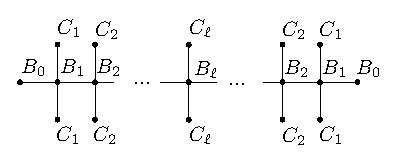
\includegraphics[width=0.4\textwidth]{symmetropillar.eps}
\]
We consider a potential on the vertices with left-right and top-bottom
mirror symmetries, and we correspondingly label equivalent vertices with
identical labels. Our potential is as follows\footnote{Curious readers
  may wonder how this potential was arrived at. One can choose a
  desired ground state and potential on the $B$ vertices, set the
  ground energy to zero, and solve for the wavefunction and potential
  on the $C$ vertices. With some trial and error one can find
  choices such that the wavefunction at $B_\ell$ is exponentially
  small, yet the potential on each $C$ vertex is greater than the
  potential on the $B$ vertex to which it is connected and the ground
  state amplitudes are nonnegative on all vertices.}.
\begin{equation}
\begin{array}{rcll}
W(B_0) & = & 0 & \vspace{5pt} \\
W(B_j) & = & -\frac{1}{2} - \frac{j}{4l} & j \in \{1,\ldots,\ell\}
\vspace{5pt} \\
W(C_1) & = & \frac{1}{\frac{11}{12}-\frac{1}{8 \ell}}-1 & \vspace{5pt}\\
W(C_\ell) & = & 7 & \vspace{5pt} \\
W(C_j) & = & \frac{1}{\frac{2}{3}-\frac{j}{8 \ell}} -1 & j \in
\{2,\ldots,\ell-1\}
\end{array}
\end{equation}
One sees that this potential is a single basin funneling to the unique
minimum-potential vertex $B_\ell$. (See Fig. \ref{twopanes}.) The
following unnormalized eigenstate has eigenvalue zero.
\begin{equation}
\label{psi}
\begin{array}{rcll}
\psi(B_0) & = & \frac{2}{3} & \vspace{5pt} \\
\psi(B_j) & = & \left( \frac{2}{3} \right)^j & j \in \{1,\ldots,\ell\}
\vspace{5pt} \\
\psi(C_\ell) & = & \frac{1}{8} \left( \frac{2}{3} \right)^\ell &
\vspace{5pt} \\
\psi(C_1) & = & \frac{2}{3} \left( \frac{11}{12}-\frac{1}{8 \ell}
\right)  & \vspace{5pt} \\
\psi(C_j) & = & \left( \frac{2}{3}-\frac{j}{8 \ell} \right) \left(
  \frac{2}{3} \right)^j & j \in \{2,\ldots,\ell-1\}
\end{array}
\end{equation}
All off-diagonal elements of the Hamiltonian $H_{G,W}$ are
nonpositive. Therefore, by the Perron-Frobenius theorem, its ground
state is the only eigenstate with all nonnegative amplitudes
\cite{BDOT08}. Hence, we can identify $\psi$ as the ground state of
$H_{G,W}$.

\begin{figure}
\begin{center}
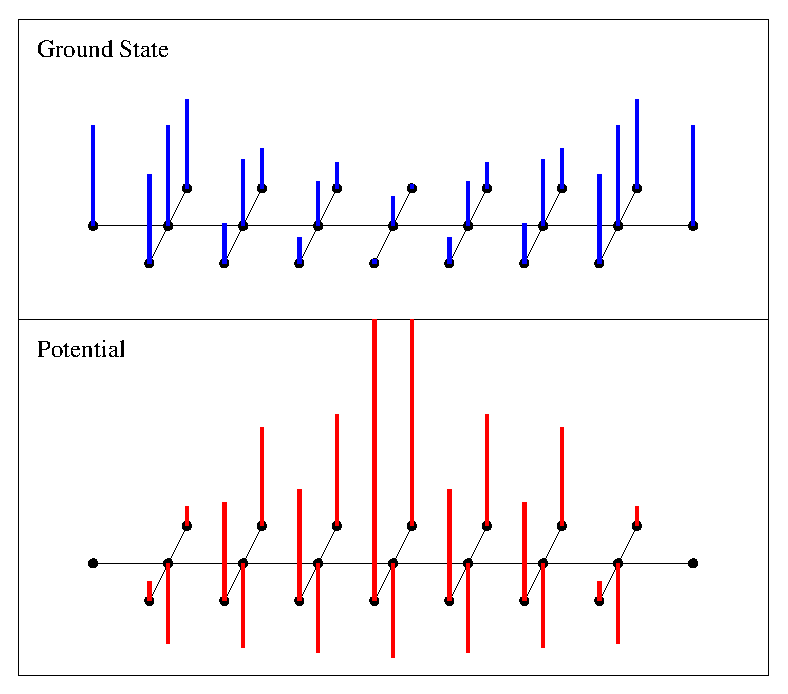
\includegraphics[width=0.65\textwidth]{twopanes.eps}
\caption{\label{twopanes} We illustrate the ground state wavefunction
  $\psi$ and the 
  potential $W$ for $\ell = 4$. The ground state $\psi$ consists
  of two lobes separated by a region of small amplitude in the
  center. The potential along the ``spine'' of the caterpillar is
  negative and decreasing as one approaches the central vertex
  $B_4$. The  potential is positive on the ``legs'' of the
  caterpillar. Thus, the classical steepest-descent algorithm starting
  from any initial vertex will reach the minimum ($B_4$) by the
  shortest path. Note that the potential on the $C_4$ vertices is
  approximately ten times as large as the second largest value of the
  potential, and thus it is cut off by the boundaries of the figure.}
\end{center}
\end{figure}

A ground state consisting of two symmetric lobes, such as $\psi$,
implies a small eigenvalue gap because, by flipping the signs of the
amplitudes in one lobe, one obtains an orthogonal state of only
slightly higher energy. This energy cost, which upper-bounds the
eigenvalue gap, is small due to the smallness of the amplitudes
between the lobes.

More precisely, consider the wavefunction $\phi$, which equals $\psi$ for all
vertices to the left of $B_{\ell}$, equals $-\psi$ for all vertices
to the right of $B_{\ell}$, and equals zero at $B_{\ell}$ and
$C_\ell$. One sees that $\phi$ is orthogonal to $\psi$. Let $\eta =
\braket{\phi}{\phi}$ and let $\ket{\widetilde{\phi}} =
\frac{1}{\sqrt{\eta}} \ket{\phi}$ be the normalized version of
$\ket{\phi}$. The first excited state is variationally characterized
as the lowest energy state orthogonal to the ground state. Therefore
the energy of the first excited state is at most
$\bra{\widetilde{\phi}} H_{G,W} \ket{\widetilde{\phi}}$. Because the
ground energy is zero we thus have
\begin{equation}
\label{gammaphi}
\gamma \leq \bra{\widetilde{\phi}} H_{G,W} \ket{\widetilde{\phi}}.
\end{equation}

By construction, $\ket{\phi}$ satisfies the 
eigenvalue zero equation everywhere except at the $B_{\ell}$ vertex
and the two $B_{\ell-1}$ vertices. Using this fact, one finds
\begin{equation}
\bra{\phi} H_{G,W} \ket{\phi} = 2 \psi(B_{\ell}) \psi(B_{\ell-1}).
\end{equation}
By (\ref{psi}) one sees that $\eta > 1$. Therefore,
(\ref{gammaphi}) yields 
\begin{eqnarray}
\gamma & \leq & 2 \eta^{-1} \psi(B_{\ell})\psi(B_{\ell-1}) \\
       & < & 2 \psi(B_{\ell}) \psi(B_{\ell-1}) \\
       & = & 2 \left( \frac{2}{3} \right)^{2\ell-1}.
\end{eqnarray}
Hence, without any local minima in the potential and with only
$O(\ell)$ vertices we obtain an eigenvalue gap of $O((2/3)^{2\ell})$. 

\section{Conductance-based Gap Bounds}
\label{sec:conductance}

In the preceding section, we showed that a ground state consisting of
two symmetric lobes separated by a region of small amplitude implies a
small eigenvalue gap. We relied on the symmetry of the lobes to
construct a low-energy state orthogonal to the ground state by
flipping the sign of the amplitudes on one lobe. However, it is true
more generally that lobes separated by a region of small amplitude
imply a small gap even if the lobes are asymmetric, provided the
imbalance is not too severe. In this section we use concept of
conductance to make this precise, and conversely to prove that if the
ground state wavefunction is single-peaked, then the eigenvalue gap
cannot be smaller than $\Omega(|V_G|^{-2})$.

\subsection{Conductance}
\label{subsec:conductance}

Motivated by applications to rapidly mixing Markov chains,
sophisticated tools have been developed to bound the difference
between the largest and second-largest eigenvalues of stochastic 
matrices. In this subsection, we recount one such tool, known as
conductance.

Consider a discrete-time random walk on $G$ defined by transition
matrix $P$. That is, for $x,y \in V_G$, $P_{xy}$ is the
probability for a walker at $x$ to transition to $y$ in
a given timestep. Thus, $P$ is a row-stochastic matrix. Conductance
provides upper and lower bounds on the gap between the largest and
second largest eigenvalues of row-stochastic matrices in the case that
the random walks they define are ergodic and reversible. Ergodicity means
that the random walk converges to the same limiting distribution
independent of the starting point of the walker. Reversibility means
that, in the limiting distribution, the probability of traversing a
given edge in one direction is equal to the probability of traversing
it in the opposite direction. More formally, we recount the following
definitions and facts from \cite{Sinclair}.

\begin{definition}
The random walk defined by transition matrix $P$ on vertex set $V_G$
is ergodic if
\begin{equation}
\lim_{s \to \infty} \left( P^s \right)_{xy} = \pi_y \quad
\textrm{independent of $x$}.
\end{equation}
The probability distribution $\pi$ is then called the limiting
distribution of the random walk.
\end{definition}

\begin{lem}
\label{ergodicity}
The following conditions are necessary and sufficient for ergodicity
of $P$.
\begin{enumerate}
\item $P$ is irreducible. That is, for each $x,y \in V_G$ there is $s
  \in \mathbb{N}$ such that $\left( P^s \right)_{xy} > 0$.
\item $P$ is aperiodic. That is, for all $x,y$, $\mathrm{gcd} \{ s|
  (P^s)_{xy} > 0 \} = 1$.
\end{enumerate}
\end{lem}

\begin{definition}
An ergodic random walk given by transition matrix $P$ on vertex set
$V_G$ is reversible if
\begin{equation}
\pi_x P_{xy} =  \pi_y P_{yx} \quad \forall x,y \in V_G,
\end{equation}
where $\pi$ is the limiting distribution.
\end{definition}

\begin{definition}
Let $P$ be the transition matrix of a reversible ergodic random walk
on graph $G$ with vertices $V_G$ and edges $E_G$. Let $\pi$ be the
corresponding limiting distribution. Let $S$ be any non-empty subset
of $V_G$ and let $\bar{S} = V_G/S$ be its complement. Let
\begin{eqnarray}
F_S & = & \mathop{\sum_{(x,y) \in E_G}}_{x \in S, y \in \bar{S}} \pi_x
P_{xy} \vspace{30pt} \\[5pt]
C_S & = & \sum_{x \in S} \pi_x \\[5pt]
\Phi_S(P) & = & \frac{F_S}{\min\{C_S, C_{\bar{S}}\}} \\[5pt]
\Phi(P) & = & \min_{S \subset V_G} \Phi_S(P).
\end{eqnarray}
$\Phi(P)$ is called the conductance of $P$.
\end{definition}

The quantity $F_S$ is called the flow of $S$, and the quantity $P_S$
is called the probability of $S$. Note that, for reversible random
walks, $F_S = F_{\bar{S}}$. By the Perron-Frobenius theorem, the
largest eigenvalue of any irreducible stochastic matrix is 1 and the
corresponding eigenspace is one-dimensional. Furthermore, this
eigenvector can be written with all nonnegative entries. Adapting
theorems 2.4 and 2.6 of \cite{Sinclair} one has the following.

\begin{lem}
\label{conductance}(from \cite{Sinclair})
Let matrix $P$ define a reversible ergodic random walk with
conductance $\Phi(P)$. Let $\gamma$ denote the gap between the largest
eigenvalue of $P$ (which is 1) and the second-largest eigenvalue. Then
\begin{equation}
\frac{\Phi(P)^2}{2} \leq \gamma \leq 2 \Phi(P).
\end{equation}
\end{lem}

Proposition \ref{conductance} is based on Cheeger's inequality
\cite{Cheeger} for the spectrum of Laplacians of manifolds, which was
adapted to graphs by Alon and Milman \cite{Alon}, and extended to
stochastic matrices by Sinclair \cite{Sinclair}.

\subsection{Conductance Bound}
\label{sec:general}

In this subsection we use conductance to prove lower bounds on the gap
of Hamiltonians of the form $H_{G,W}$ given in (\ref{HGW}),
culminating in a proof that the ``lobed'' nature of the ground state
wavefunction in the counterexample from \S \ref{counter} is a
necessary feature to obtain exponentially small gap. Specifically, we
show that if $H_{G,W}$ has a single-peaked ground state then its
eigenvalue gap has an $\Omega(|W|^{-1} |V_G|^{-2})$ lower bound, where
$|V_G|$ is the number of vertices in the graph $G$ and $|W| =
\max_{x\in V_G} W(x) - \min_{x \in V_G} W(x)$.

Given a connected graph $G$, and a potential $W$ on the vertices, let
$H_{G,W}$ be the corresponding Hamiltonian of the form (\ref{HGW}).
Let $\gamma$ denote the energy gap between the ground state and first
excited state of $H_{G,W}$. For the purpose of bounding $\gamma$ we
may assume without loss of generality that the potential satisfies
$W(x) < -d_G \quad \forall x \in V_G$, where $d_G$ is the maximum degree
of any vertex in $G$. If this is not the case, one can always
subtract a sufficiently large multiple of the identity matrix to make
it so without affecting $\gamma$.

Let $\ket{\psi} = \sum_{x \in V_G} \psi(x) \ket{x}$ denote the ground
state of $H_{G,W}$ and $E$ the ground energy. Let $N_x$ be the
neighbors of vertex $x$. That is, 
\begin{equation}
N_x = \{ y \in V_G| (x,y) \in E_G\}.
\end{equation}
In this notation,
\begin{equation}
\label{eigen1}
 (d_x +W(x)) \psi(x) - \sum_{y \in N_x} \psi(y) = E \psi(x).
\end{equation}
For connected $G$, 
\begin{equation}
\label{strictly}
\psi(x) > 0 \quad \forall x.
\end{equation}
Thus we may rearrange
(\ref{eigen1}) to obtain
\begin{equation}
\label{eigen2}
d_x + W(x) -\sum_{y \in N_x} \psi(y)/\psi(x)  = E.
\end{equation}
Also, note that $H$ has all nonpositive entries, so $E < 0$. 

We next adapt a technique from \cite{ATS03, BT09, AP10} to relate the
spectrum of $H_{G,W}$ to the spectrum of a random walk. Let $D =
\mathrm{diag}\{\psi(x)|x \in V_G\}$. By (\ref{strictly}), $D$ is an
invertible matrix with $D^{-1} = \mathrm{diag}\{\psi(x)^{-1}|x \in
V_G\}$. Let
\begin{equation}
\label{Pdef}
P = \frac{1}{E} D^{-1} H_{G,W} D.
\end{equation}
By (\ref{eigen2}), $\sum_{y \in V_G} \bra{x} P \ket{y} = 1$. That is,
$P$ is a row-stochastic matrix.

Because $E < 0$, the lowest eigenvalue of $H$ corresponds to the
highest eigenvalue of $P$, which is 1. Specifically, let
\begin{equation}
\ket{\psi^2} = \sum_{x \in V_G} \psi(x)^2 \ket{x}.
\end{equation}
One sees that
\begin{equation}
\bra{\psi^2} P = \bra{\psi^2}.
\end{equation}
Hence the probability distribution $\psi^2$ is a limiting distribution
of the random walk defined by $P$. Connectedness of the graph $G$
suffices to ensure that condition 1 of proposition \ref{ergodicity} is
satisfied. The requirement that $W(x) < -d_G$ for all $x
\in V_G$ ensures that condition 2 of proposition \ref{ergodicity} is
satisfied \cite{Sinclair}. Thus, $P$ is an ergodic random walk. In
other words, $\psi^2$ is the unique limiting distribution of $P$ and
correspondingly $\ket{\psi}$ is the nondegenerate ground state of
$H_{G,W}$. By direct calculation, one finds
\begin{equation}
\psi(x)^2 P_{xy} = \psi(y)^2 P_{yx} = \left \{ \begin{array}{cl}
-\frac{1}{E} \psi(x) \psi(y) & \textrm{if $(x,y) \in E_g$}\\
0 & \textrm{otherwise}.
\end{array} \right.
\end{equation}
Thus, $P$ is a reversible ergodic random walk. Therefore, by
proposition \ref{conductance} and equation (\ref{Pdef}), the energy
gap $\gamma$ between the ground and first-excited states of $H_{G,W}$
satisfies
\begin{equation}
\label{bounds}
-\frac{E}{2} \Phi^2(P) \leq \gamma \leq -2E \Phi(P).
\end{equation}
One sees that the flow between $S \subset V_G$ and its complement
determined by $P$ is
\begin{equation}
F_S(P) = \mathop{\sum_{x \in S}}_{y \in \bar{S}} \frac{\psi(x)
  \psi(y)}{-E}
\end{equation}
and the corresponding probability is
\begin{equation}
C_S(P) = \sum_{x \in S} \psi(x)^2.
\end{equation}
Thus, by (\ref{bounds}) one obtains the following result.
\begin{lem}
\label{mainlemma}(cf. \cite{ATS03, BT09, AP10})
Let $H_{G,W}$ be a Hamiltonian of the form (\ref{HGW}) with $W(x) \leq
-d_G \quad \forall x \in V_G$. Let $\psi$ denote the ground state of
$H_{G,W}$, let $E$ denote the ground energy, and let $\gamma$ denote
the gap between the ground energy and the first excited energy. Then,
\begin{equation}
\label{lowerbound}
 - \frac{1}{2E} \Phi_H^2 \leq \gamma \leq 2 \Phi_H
\end{equation}
where
\begin{eqnarray}
\Phi_H & = & \min_{S \subset V_G} \frac{F_S}{\min
    \{C_S, C_{\bar{S}}\} } \\
F_S & = & \sum_{(x,y) \in B} \psi(x) \psi(y) \label{ar1}\\
B   & = & \{(x,y)| x \in S, y \notin S, (x,y) \in E_G\} \label{ar2}\\
C_S & = & \sum_{x \in S} \psi(x)^2 \label{ar3}\\
C_{\bar{S}} & = & \mathop{\sum_{x \in V_G}}_{x \notin S} \psi(x)^2. \label{ar4}
\end{eqnarray}
\end{lem}
\noindent
Note that $E < 0$ and therefore the lower bound on $\gamma$ given by
(\ref{lowerbound}) is nonnegative.

Examining (\ref{lowerbound}) one sees that the gap is exponentially
small if and only if the ground state has a pair of 
not-too-unbalanced lobes separated by a region of exponentially small
amplitude. Choosing $S$ and $\bar{S}$ to be the lobes, one sees that
$S$ and $\bar{S}$ must have reasonably well-balanced ground state
probabilities for the denominator $\min\{C_S, C_{\bar{S}}\}$ to remain
large, and the amplitudes along the cut separating $S$ from $\bar{S}$
must all be small for the numerator $F_S$ to be small. More precisely,
recalling from \S \ref{sec:preliminaries} the definition of
single-peaked, we have the following, which is the main result of this
section.

\begin{lem}
\label{mainprop}
Let $G$ be a connected graph with vertices $V_G$, edges $E_G$, and
maximum degree $d_G$. Let $W:V_G \to \mathbb{R}$ be a potential, and
$H_{G,W}$ the corresponding Hamiltonian described in (\ref{HGW}). Let
$\psi$ denote the ground state of $H_{G,W}$ and let $\gamma$ denote
the eigenvalue gap between the ground state and first excited state of
$H_{G,W}$. If $\psi$ is single-peaked then
\begin{equation}
\gamma \geq \frac{1}{2 (|W|+d_G) |V_G|^2}
\end{equation}
where
\begin{equation}
|W| = \max_{x \in V_G} W(x) - \min_{x \in V_G} W(x).
\end{equation}
\end{lem}

\noindent
\begin{proof}
Let 
\begin{equation}
    H_{G,W}^{(-)} = H_{G,W} - (W_{\max}+d_G) \id
\end{equation} 
where $W_{\max} = \max_{x \in V_G} W(x)$. One sees that
$H_{G,W}^{(-)}$ has the same ground state $\psi$ and same gap $\gamma$
as $H_{G,W}$ and that all matrix elements in $H_{G,W}^{(-)}$ are
nonpositive. Hence, by 
proposition \ref{mainlemma},
\begin{equation}
\label{first}
\gamma \geq - \frac{1}{2E^{(-)}} \left( \min_{S \subset V_G} \frac{F_S}{\min\{C_S,
    C_{\bar{S}}\}} \right)^2
\end{equation}
where $E^{(-)}$ is the ground energy of $H_{G,W}^{(-)}$, namely
\begin{equation}
E^{(-)} = E - (W_{\max}+d_G),
\end{equation}
and $F_S$, $C_S$, and $C_{\bar{S}}$ are as in
(\ref{ar1})-(\ref{ar4}). Graph Laplacians are positive semidefinite,
and therefore $E \geq W_{\min}$. Thus,
\begin{equation}
E^{(-)} \geq -|W|-d_G.
\end{equation}
Hence, (\ref{first}) yields
\begin{equation}
\label{second}
\gamma \geq \frac{1}{2(|W|+d_G)} \left( \min_{S \subset V_G}
  \frac{F_S}{\min\{C_S, C_{\bar{S}}\}} \right)^2.
\end{equation}
We now consider two cases: 1) the peak of $\psi$ spans the
cut $\{S,\bar{S}\}$, and 2) the peak of $\psi$ is contained entirely
within one side of the cut.\\
\textbf{Case 1:}
If the peak of $\psi$ spans the cut then there exist $x \in S$ and $y
\in \bar{S}$ such that $(x,y) \in E_G$ and $\psi(x) = \psi(y) \geq
\psi(z) \ \forall z \in V_G$. We can lower bound $\gamma$ by throwing
away the flows across all edges in the numerator other than
$(x,y)$. Thus,
\begin{equation}
\gamma \geq \frac{1}{2(|W|+d_G)} \left( \frac{\psi(x)^2}
{\min\{C_{S},C_{\bar{S}}\}} \right)^2.
\end{equation}
Furthermore, $\min\{C_{S},C_{\bar{S}}\} \leq \psi(x)^2 |V_G|$,
and therefore $\gamma \geq \frac{1}{2 (|W|+d) |V_G|^2}$.\\
\textbf{Case 2:}
If the peak of $\psi$ is contained within one side of the cut, we may,
without loss of generality, call the side containing the peak $S$ and
the other side $\bar{S}$. Let $x_{\max}$ be the vertex in $\bar{S}$
that maximizes $\psi$. Because $\psi$ is single-peaked, there must be
a neighbor $z$ of $x_{\max}$ such that $\psi(z) >
\psi(x_{\max})$. Because $\psi(x_{\max})$ maximizes $\psi$ in
$\bar{S}$, $z$ must be contained in $S$. We can lower bound $\gamma$
by throwing away the flows across all edges in the numerator other
than $(x_{\max},z)$. Thus,
\begin{equation}
\gamma \geq \frac{1}{2(|W|+d_G)} \left( \frac{\psi(x_{\max}) \psi(z)}
{\min\{C_{S},C_{\bar{S}}\}} \right)^2
\geq \frac{1}{2(|W|+d_G)} \left( \frac{\psi(x_{\max})^2}
{\min\{C_{S},C_{\bar{S}}\}} \right)^2.
\end{equation}
Furthermore, $C_{\bar{S}} \leq \psi(x_{\max})^2 |V_G|$, and therefore
$\min\{C_{S},C_{\bar{S}}\} \leq \psi(x_{\max})^2 |V_G|$. 
Thus, in this case also, $\gamma \geq \frac{1}{2 (|W|+d_G) |V_G|^2}$.
\end{proof}

\subsection{Conductance Bound for Path Graphs}
\label{conductance1D}

Here we note some consequences of proposition \ref{mainprop} in the
case that $G$ is the path graph of $l$ vertices, $G_l$.
\[
\begin{array}{rcl}
G_l & = & 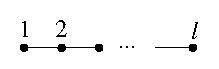
\includegraphics[width=0.2\textwidth]{path.eps}
\end{array} \vspace{10pt}
\]

\begin{definition}
Let $G$ be a graph with vertices $V_G$ and edges $E_G$. Let $W:V_G \to
\mathbb{R}$ be a potential. We say $W$ is a single-basin potential
if the set $\{x \in V_G| W(x) < E\}$ is a connected set of vertices in
$G$ for all $E$.
\end{definition}

As we now show, single-basin potentials on the path graph have
single-peaked ground states and hence a large eigenvalue gap by
proposition \ref{mainprop}. For intuition, recall that, for a single
particle in the one-dimensional continuum, the time-independent
Schr\"odinger equation can be written as 
$-\frac{d^2 \psi}{dx^2} = (E-W(x)) \psi$. The ground state can be
expressed with all real non-negative amplitudes. Hence the sign of
$\frac{d^2 \psi}{dx^2}$ is the same as the sign of $W(x)-E$. Thus, the
ground state of a convex potential has simple structure: inside the
well, $W(x)-E < 0$ and the wavefunction is concave down, whereas
outside the well $W(x)-E > 0$ and the wavefunction is concave up. The
path graph case, described below, is essentially a discrete analogue
to this. \\

\noindent
\textbf{Remark:} The notion of a single-basin potential is
well-defined on any graph. On path graphs one can also easily
define the notion of a convex potential. Simply think of the $l$
vertices as corresponding to the integers $\{1,\ldots,l\}$ and demand
that the potential on the vertices be equal to some convex function on
$\mathbb{R}$ evaluated at these integer points. It is not hard to show
that single-basin is a slightly weaker condition than convex. That is,
on the path graph, all convex potentials are single-basin, but not all
single-basin potentials are convex. \\

For a wavefunction $\psi$ on the vertices of $G$, define
\begin{equation}
\Delta^2 \psi(x) = - d_x \psi(x) + \sum_{y \in N_x} \psi(y),
\end{equation}
where $d_x$ is the degree of vertex $x$ and $N_x$ is the set vertices
neighboring $x$. Thus, 
\begin{equation}
\label{deriv}
L_G \ket{\psi} = -\sum_{x \in V_G} \Delta^2 \psi(x) \ket{x}.
\end{equation}

\begin{lem}
Suppose $W$ is a single-basin potential on graph $G$. Let $\psi$ be
the ground state of the corresponding Hamiltonian $H_{G,W}$, and let
\begin{equation}
S[\psi] = \{x \in V_G| \Delta^2 \psi(x) < 0 \}.
\end{equation}
Then, $S[\psi]$ is a connected set of vertices in $G$.
\end{lem}

\noindent
\begin{proof}
Let $E$ denote the ground energy of $H_{G,W}$. Thus, by (\ref{deriv}),
\begin{equation}
\Delta^2 \psi(x) = (W(x)- E) \psi(x)
\end{equation}
Recall that $\psi(x) > 0 \quad \forall x \in V_G$. Thus, $\Delta^2
\psi(x)$ has the same sign as $W(x)- E$. The connectedness of
$S[\psi]$ then follows directly from the single-basin property.
\end{proof}

In special case that $G$ is a path graph, the connectedness
of $S[\psi]$ implies that $\psi$ has only one local
maximum. Thus, as a corollary of proposition \ref{mainprop}, one
obtains proposition \ref{1Dprop}. Note that on more general graphs,
connectedness of $S[\psi]$ does not imply that $\psi$ has only one
local maximum.

\begin{lem}
\label{1Dprop}
Let $W$ be a single-basin potential on the path graph $G_l$. Let
$H_{G,W}$ be the corresponding Hamiltonian of the form
(\ref{HGW}). Let $\gamma$ denote the gap between the ground energy and
first excited energy of $H_{G,W}$. Then $\gamma \geq
\frac{1}{2(|W|+2)l^2}$ where $|W| = \max_{x \in V_G} W(x) - \min_{x
  \in V_G} W(x)$.
\end{lem}

Proposition \ref{1Dprop} shows that for single-basin potentials on
$G_l$, the eigenvalue gap obeys $\gamma = \Omega(1/l^2)$. In the
special case of a flat potential, it is easy to solve for the
eigenvalue gap exactly, which is $O(1/l^2)$. However, the bound of
proposition \ref{1Dprop} is not tight due to the dependence on
$|W|$. In the next section, we obtain a tighter bound by applying
the Poincar\'e inequality.

\section{Poincar\'e-based Gap Bounds}

Two of the main tools for proving lower bounds on the eigenvalue gap
of stochastic matrices are the Cheeger inequality and the Poincar\'e
inequality. Conductance methods, such as those described in \S
\ref{subsec:conductance}, are originally derived from the Cheeger
inequality \cite{Cheeger}. For some random walks, the Poincar\'e
inequality yields stronger lower bounds than the Cheeger inequality
\cite{DS91, FW99}, and for other random walks the reverse is true
\cite{P12}. In \S \ref{sec:poincare}, we recount the version of
the Poincar\'e inequality given in \cite{DS91} and apply it to
Hamiltonians $H_{G,W}$ of the form (\ref{HGW}). In \S
\ref{sec:poinpath} we specialize to the case of path graphs, obtaining
a tighter bound than our conductance-based bound (proposition
\ref{1Dprop}). (For a previous example in which Poincar\'e's
inequality is used to bound the gap of a Hamiltonian see
\cite{BCMNS12}.)

\subsection{The Poincar\'e Inequality}
\label{sec:poincare}

Let $P$ be the transition matrix for an ergodic reversible
discrete-time random walk on a graph $G$. Let $\pi$ denote the
limiting distribution and let $\gamma$ denote the gap between the
highest and second-highest eigenvalues of $P$. For
any edge $e$ in the graph $G$, let $e_1,e_2$ denote the vertices at
its endpoints. Let $Q(e)$ denote the flow across edge $e$ in the
limiting distribution.
\begin{equation}
Q(e) = \pi_{e_1} P_{e_1,e_2} = \pi_{e_2} P_{e_2,e_1}.
\end{equation} 
The latter equality expresses the reversibility of the random walk.
For each ordered pair $(x,y)$ of distinct vertices in $G$, choose a
canonical path $\gamma_{xy}$ from $x$ to $y$. Vertices may be repeated
in a path, but no edge may be traversed more than once. Let $\Gamma$
be the collection of canonical paths, one for each ordered pair of
vertices. For
$\gamma_{xy} \in \Gamma$, let
\begin{equation}
|\gamma_{xy}| = \sum_{e \in \gamma_{xy}} Q(e)^{-1}
\end{equation}
where the sum is over the edges in path $\gamma_{xy}$. Let
\begin{equation}
\kappa(\Gamma) = \max_e \sum_{\gamma_{xy} \owns e} |\gamma_{xy}|
\pi_x \pi_y.
\end{equation}
The Poincar\'e inequality states \cite{DS91}
\begin{equation}
\label{poincare}
\gamma \geq \frac{1}{\kappa}.
\end{equation}
To obtain a tight bound on $\gamma$ one must make a good choice of
$\Gamma$.

Intuitively, the quantity $\frac{1}{\kappa}$, like the conductance
$\Phi$, quantifies the presence of a bottleneck across which the flow
is small. As an example, consider a graph consisting of two large
subgraphs connected by only a single edge $e$. In this case, every pair of
vertices spanning the pair of subgraphs has a canonical path crossing
$e$. Correspondingly, $\sum_{\gamma_{xy} \owns e} |\gamma_{xy}| \pi_x \pi_y$ will
be large, which implies large $\kappa$. Similarly, $\kappa$ will be
large if there are many edges connecting the two subgraphs to each
other but the flow $Q(e)$ across all such edges is small. Only in the
absence of such bottlenecks does (\ref{poincare}) yield a large lower
bound on the gap.

As in \S \ref{sec:general}, we use (\ref{Pdef}) to obtain a
stochastic matrix $P$ from our Hamiltonian $H$ such that the
eigenvalue gap $\gamma$ of $P$ relates to the eigenvalue gap
$\gamma_H$ of $H$ according to 
\begin{equation}
\label{gammarel2}
\gamma_H = -E \gamma,
\end{equation}
where $E$ is the ground energy of $H$. The eigenvalue gap of
$P$ can be lower-bounded using the Poincar\'e
inequality. Specifically, by (\ref{Pdef}), we have the following.
\begin{eqnarray}
Q(x,y) & = & \frac{\psi(x)\psi(y)}{-E} \\
\pi_x & = & \psi(x)^2 \\
\kappa & = & \max_e \sum_{\gamma_{xy} \owns e} \psi(x)^2 \psi(y)^2
\sum_{g \in \gamma_{xy}} \frac{-E}{\psi(g_1) \psi(g_2)}.
\end{eqnarray}
Here $\psi$ is the ground state of $H$, and $g_1,g_2$ are the two
vertices connected by edge $g$. By (\ref{gammarel2}) the ground energy
cancels from the final bound on  $\gamma_H$. Summarizing:
\begin{equation}
\label{gammahpoin}
\gamma_H \geq \frac{1}{\kappa'},
\end{equation}
where
\begin{equation}
\label{kappaprime}
\kappa' = \max_e \sum_{\gamma_{xy} \owns e} \psi(x)^2 \psi(y)^2
\sum_{g \in \gamma_{xy}} \frac{1}{\psi(g_1) \psi(g_2)}.
\end{equation}

\subsection{Poincar{\'e} Bound for Path Graphs}
\label{sec:poinpath}

For path graphs, there is only one valid choice of canonical paths
$\Gamma$. Specifically, for a pair of vertices $s < f$ the canonical
path is $s,s+1,\ldots,f$. For $f < s$ one takes the reverse
path. Thus, (\ref{kappaprime}) reduces to 
\begin{equation}
\label{simprime}
\kappa' = \max_{1 \leq j \leq l-1} 2 \sum_{s \leq j} \sum_{f > j}
R(s,f)
\end{equation}
where
\begin{equation}
\label{RSF}
R(s,f) = \psi(s)^2 \psi(f)^2 \sum_{s \leq v < f} \frac{1}{\psi(v) \psi(v+1)}.
\end{equation}
The factor of 2 in (\ref{simprime}) arises because we sum only over
the paths with $s < f$ and use the fact that $R(s,f) = R(f,s)$.
 
As discussed in \S \ref{conductance1D}, if the potential on the
path graph is single-basin, then the ground state wavefunction has only one
local maximum. Thus, the minimum of $\psi(v)$ along a segment $s \leq
v < f$ must occur at one of the endpoints. If the minimum is at $s$
then (\ref{RSF}) yields
\begin{eqnarray}
R(s,f) & \leq & \psi(s)^2 \psi(f)^2 \sum_{s \leq v < f}
\frac{1}{\psi(s)^2} \\
& = & (f-s) \psi(f)^2.
\end{eqnarray}
Similarly, if the minimum is at $f$ then one has $R(s,f) \leq (f-s)
\psi(s)^2$.

Let $J$ be the value of $j$ that achieves the maximum in
(\ref{simprime}). Then
\begin{equation}
\kappa' \leq 2 \sum_{s \leq J} \sum_{f > J}  (f-s) \psi(b_{s,f})^2
\end{equation}
where $b_{s,f}$ is either $s$ or $f$ depending on which is smaller amongst
$\psi(s)^2$ and $\psi(f)^2$. We can rewrite this sum over pairs of
vertices as
\begin{equation}
\label{rejigger}
\sum_{s \leq J} \sum_{f > J}  (f-s) \psi(b_{s,f})^2 = \sum_{b=1}^l
\sum_{a \in S_b} |a-b| \psi(b)^2,
\end{equation}
where, for a given vertex $b$, $S_b$ is the set of
vertices on the other side of edge $J$ such that $\psi(a)^2 \leq
\psi(b)^2$. (For some $b$, $S_b$ can be empty.) From (\ref{rejigger})
we have
\begin{eqnarray}
\kappa' & \leq & 2 \sum_{b=1}^l \psi(b)^2 \sum_{a \in S_b} |a-b| \\
        & \leq & 2 \sum_{b=1}^l \psi(b)^2 \sum_{a=1}^{l-1} a \\
        & =    & \sum_{b=1}^l \psi(b)^2 l(l-1) \\
        & \leq & l (l-1).
\end{eqnarray}
The last equality follows from the fact that $\psi(b)^2$ is a
probability distribution over $1,\ldots,l$. Thus, by
(\ref{gammahpoin}),
\begin{equation}
\label{final}
\gamma_H \geq \frac{1}{l(l-1)}.
\end{equation}
By direct calculation, one finds that the eigenvalue gap for the
length $l$ chain with no potential ($W=0$) is $4 \sin^2 \left(
  \frac{\pi}{2 l} \right)$. Thus, the bound (\ref{final}) is
asymptotically tight to within a factor of $\pi^2$
\cite{Jarret_Jordan}.

\section{Application to Adiabatic Optimization Algorithms}
\label{aqc}

In this section, we show that, as a corollary of proposition
\ref{mainprop}, adiabatic optimization algorithms in which the ground
state $\psi(s)$ is single-peaked for all $s$, have minimum gap at
least $\Omega(1/|V_G|^2)$ and therefore run in
$\widetilde{O}(|V_G|^4)$ time, by an adiabatic theorem
\cite{Elgart_Hagedorn}. (The $\widetilde{O}$ notation indicates that we
are omitting logarithmic factors.) This result cannot be used directly
to find algorithmic speedups, as exhaustive search runs in $O(|V_G|)$
time. However, we believe this analysis may be useful in cases of high
symmetry such as \cite{R04, DMV01, FGG02}, where the eigenvalue gap
on exponentially large graphs can be determined by analyzing the spectrum
of polynomial-size graphs. In addition, the analysis in this section
provides an illustrative example of how proposition \ref{mainprop} may
be applied to the analysis of adiabatic optimization problems.

Consider an adiabatic optimization algorithm using a Hamiltonian
$H_{G,W}(s)$ of the form shown in (\ref{HGWS}). Then 
\begin{equation}
\hat{H}_{G,W}(s) = \frac{1}{1-s} H_{G,W}(s)
\end{equation}
is of the form (\ref{HGW}) addressed by proposition
\ref{mainprop}. $\hat{H}_{G,W}(s)$ and $H_{G,W}(s)$ have the same
ground state, which we denote $\psi(s)$. Thus, if $\psi(s)$ is
single-peaked for all $s \in [0,1)$ we may conclude from proposition
\ref{mainprop} that
\begin{equation}
\label{raw_conclusion}
\hat{\gamma}(s) \geq \frac{1}{2 \left( |\hat{W}(s)|+d_G \right) |V_G|^2},
\end{equation}
where $\hat{W}(s) = \frac{s}{1-s}W$ is the potential in
$\hat{H}_{G,W}(s)$. Hence, one substitutes $|\hat{W}(s)| =
\frac{s}{1-s} |W|$ and $\gamma(s) = (1-s) \hat{\gamma}(s)$ into
(\ref{raw_conclusion}), obtaining 
\begin{equation}
\label{gammabound}
\gamma(s) \geq \frac{1-s}{2 \left( \frac{s}{1-s} |W| + d_G \right)
  |V_G|^2}.
\end{equation} 

One sees that this lower bound on $\gamma(s)$ becomes very small as
$s$ closely approaches 1. For the final part of the adiabatic
optimization algorithm we therefore use a different method to
lower-bound the eigenvalue gap. As an illustrative example, we suppose
that the gap between the minimum of $W$ and the second smallest value
taken by $W$ is one. Thus, by (\ref{HGWS}), $\gamma(1) =
1$. Generalization to other values of $\gamma(1)$ is straightforward and
yields the same scaling with $|V_G|$ and $d_G$. At $s = 1 - \delta$,
one has
\begin{equation}
H(s) = \delta L_G + (1-\delta) W.
\end{equation}
By Gershgorin's circle theorem, one sees that the operator norm of
$L_G$ is at most $2 d_G$. Thus, the operator norm of $\delta L_G$ is
at most $2 \delta d_G$. Hence, Weyl's inequalities show that the worst
case is that the addition of $\delta L_G$ to $(1-\delta)W$ shifts the
ground energy up by $2 \delta d_G$ and shifts the first excited energy
down by $2 \delta d_G$. Thus, adding $\delta L_G$ to $(1-\delta) W$ at
worst decreases the gap from $1-\delta$ to $1-\delta-4 \delta
d_G$. Thus,
\begin{equation}
\gamma(s) \geq \frac{1}{2}-\frac{1}{8 d_G} \quad \forall s \in
\left[1-\frac{1}{8 d_G},1\right].
\end{equation}
The degree $d_G$ is at least 2 for any connected graph of more than
two vertices, so for all nontrivial cases one has
\begin{equation}
\label{gammaend}
\gamma(s) \geq \frac{7}{16} \quad \forall s \in
\left[1-\frac{1}{8 d_G},1\right].
\end{equation}
For the remaining values of $s$, (\ref{gammabound}) yields
\begin{equation}
\label{gammastart}
\gamma(s) \geq \frac{\frac{1}{8 d_G}}
{2 \left( 8 d_G |W| + d_G \right) |V_G|^2} 
\quad \forall s \in \left[0,1-\frac{1}{8 d_G} \right].
\end{equation}
Together, (\ref{gammaend}) and (\ref{gammastart}) yield
\begin{equation}
\label{allgamma}
\gamma(s) = \Omega \left( \frac{1}{d_G^2 |W| |V_G|^2} \right)
\quad \forall s \in [0,1].
\end{equation}
The adiabatic theorem of \cite{JRS07} shows that adiabaticity will be
maintained by evolving according to the linear-interpolation
Hamiltonian $H_{G,W}(t/\tau)$ with runtime $\tau$ bounded by
\begin{equation}
\label{runtime}
\tau = O \left( \frac{ \left\| \frac{dH}{ds} \right\|^2}{\gamma^3} \right).
\end{equation}
By (\ref{HGWS}), $\left\| \frac{dH}{ds} \right\| = O(d_G + |W|)$. Thus,
by (\ref{allgamma}) and (\ref{runtime}),
\begin{equation}
\tau = O \left( d_G^6 |W|^3 |V_G|^6 (|W|+d_G)^2 \right).
\end{equation}

As shown in \cite{Elgart_Hagedorn}, a tighter bound on running time
can be obtained by choosing a more optimized interpolation schedule
between the initial and final Hamiltonians. Specifically, one should
choose the interpolation such that $H(t)$ is infinitely differentiable
but is time-independent outside of $t \in [0,\tau]$. For example,
let
\begin{equation}
H(t) = (1-s(t/\tau)) L_G + s(t/\tau) W
\end{equation}
where $s$ is the following ``switching function'', which is infinitely
differentiable, and satisfies $s(0) = 0$, $s(1) = 1$, and
$s'(x) = 0 \  \forall x \notin (0,1)$:
\begin{eqnarray}
s(x) & = & \int_{-\infty}^x g(y) dy \\
g(y) & = & \left\{ \begin{array}{ll}
0 & \textrm{if $y \notin [0,1]$} \\
\beta \exp \left( - \frac{1}{y(1-y)} \right) & \textrm{if $y \in (0,1)$}
\end{array} \right. . \\
\end{eqnarray}
Here, $\beta$ is the normalization constant yielding $f(1) = 1$.
In this case, as shown in \cite{Elgart_Hagedorn}, by evolving with
$H(t)$ from time zero to $\tau$ one achieves adiabaticity with
runtime
\begin{equation}
\label{switching_adiabatic}
\tau = O\left( \frac{(\log(1/\gamma))^{12}}{\gamma^2} \right).
\end{equation}
For a Hamiltonian in which the ground state is always single-peaked,
(\ref{switching_adiabatic}) and (\ref{allgamma}) yield runtime
\begin{equation}
\label{fast}
\tau = \widetilde{O}(V_G^4).
\end{equation}

\section{Concluding Remarks}

The examples analyzed here and in \cite{R04, DMV01, FGG02, VDV03,
  aminchoi} show that quantum adiabatic algorithms can succeed in
finding the minimum in polynomial time in cases where classical local
search fails to do so, and it can fail in cases where classical local
search succeeds. For both classical local search and adiabatic
optimization, local minima of the potential that one is seeking to
minimize play an important role in determining runtime. However, as
the present work shows, these local minima do not tell the whole
story. In particular, absence of local minima does not imply large
eigenvalue gap.

In addition, we note that there remains much to be learned regarding
the performance of adiabatic optimization algorithms relative to
classical computation in the general case that one is not comparing
only to classical local search. In particular, the classical algorithm
described in appendix A of \cite{childswalk} finds the minimum in
polynomial time for most of the known examples in which adiabatic
optimization beats classical local search. We hope that the tools
developed here will be helpful in investigating this issue.\\ 

\noindent
\textbf{Acknowledgments: }We thank Amanda Streib, Noah Strieb, and
Alexey Gorshkov for useful conversations. Portions of this paper are a
contribution of NIST, an agency of the US government, and are not
subject to US copyright. This work was supported in part by the center
for Quantum Information and Computer Science (QuICS).



\crefname{secinapp}{appendix}{appendices}
\Crefname{secinapp}{Appendix}{Appendices}

\newtheorem{fact}{Fact}

\newcommand{\size}[1]{\left\lvert #1 \right\rvert}
\newcommand{\graph}[2]{\mathbb{#1}_{#2}}
\newcommand{\intset}[2]{\left \llbracket #1 , #2 \right \rrbracket}

\chapter{One dimensional fundamental gap theorem}

\section{Introduction}
  The Fundamental Gap Conjecture proposed a tight lower bound of $3\pi^2/D^2$ to the difference between the two lowest eigenvalues (the gap) of a Schr\"{o}dinger operator $-\nabla^2 + V(x)$ with convex potential $V$ on a compact convex domain $\Omega \subset \mathbb{R}^n$ of diameter $D$ and subject to Dirichlet boundary conditions. Recently, Andrews and Clutterbuck proved the conjecture for all ``semiconvex'' potentials (which include convex potentials as a special case) in arbitrary dimensions \cite{Andrews2011}. Although the community's focus has largely centered on the continuum\cite{Andrews2011, Lavine1994, ashbaugh1989optimal, Yu1986}, as early as 1990 Ashbaugh and Benguria saw the potential for extending their results to discrete Laplacians. In their work, they proved a lower bound to the gap for a particular class of discrete Laplacians with symmetric-decreasing potentials \cite{ashbaugh1990some}. Indeed, recent interest in adiabatic quantum computing justifies their vision and motivates our interest in lifting continuum results to graph Laplacians\cite{Farhi_science, FGG02}. While our interest is driven by quantum computation, the discrete eigenvalue gap is also of interest to condensed matter physicists. Abstractly, this result is a useful addition to spectral theory.

  Previously, in the setting of quantum computation, gap bounds were derived on an as-needed basis. For instance, in an analysis of the power of adiabatic algorithms, van Dam et al. bounded eigenvalue gaps in the minimum Hamming weight problem by considering an explicit gap and then bounding the maximum error on this gap from perturbations\cite{DMV01}. In another instance, Reichardt considers the eigenvalue gap for an Ising system by using properties of the operator's principal submatrices\cite{R04}. (At least in the case of the path graph, Reichardt's Sturm sequences are similar in form to our eigenvector recurrence of \cref{eqn:recurrence}. For an explicit examination of the link between principal submatrices and the eigenvector recurrences, see Gantmakher and Kre\u{i}n\cite{gantmakher2002oscillation}.) Unlike the constructions above, we look to develop tools of increasingly general applicability. Thus, we begin with systems where gaps are demonstrably ``large'' and search for extensions of these systems to problems of algorithmic and physical interest.

  In this work, we consider specifically Schr\"{o}dinger operators corresponding to graph Laplacians with suitably defined convex potential terms. Here, the potential is restricted to the vertices and can be seen either as a site-dependent physical potential (as in the physics literature) or as a weighted graph with loops (as in the mathematical and computer science literature). Thus, for a graph $\mathbb{G}=(V,E)$ with graph Laplacian $\mathbf{L(\mathbb{G})}$ and subjected to a potential $W(\cdot)$ we consider Schr\"{o}dinger operators of the form
  \begin{equation}
    \mathbf{H}_{W}(\mathbb{G}) = \mathbf{L(\mathbb{G})} + \mathbf{W}
  \end{equation}
  where
  \begin{equation}
    \big[\mathbf{W}(V)\big]_{ij} = W(V_i) \delta_{ij}.
  \end{equation}
%redefine above.
  Although our problem is analogous to the Fundamental Gap Conjecture as proven in the continuum, lifting existing results to the discrete realm and maintaining tight bounds is non-trivial. Perhaps the most obvious challenge we face is the loss of well-defined boundary conditions and, for this reason, we restrict our initial study to the path and hypercube graphs. In the first case, our restriction gives boundary conditions similar to Neumann boundary conditions in the continuum and thus our result bears some resemblance to the continuum one of Payne and Weinberger \cite{Payne1960} and indeed converges upon this result asymptotically. (For the physicist, our path graph Hamiltonian can be viewed as a 1-dimensional chain with a nearest-neighbor interaction term and a convex, site-dependent potential term. See \Cref{fig:path}. Up to an identity term, the Laplacian of the hypercube graph of $2^N$ vertices,  $\mathbb{H}_{2^N}$, is equivalent to a sum of the Pauli $\sigma_x$ operators acting on each of $N$ qubits. In particular, transverse Ising models such as those studied in \cite{Farhi_science} can be cast as potentials on the hypercube. Here, like Reichardt\cite{R04} and van Dam et al. \cite{DMV01}, but unlike Farhi et al.\cite{Farhi_science}, we focus on the case that the potential depends only on the Hamming distance from a minimum. For the hypercube graph see \Cref{fig:path}.)
  
  \begin{figure}[htp]
    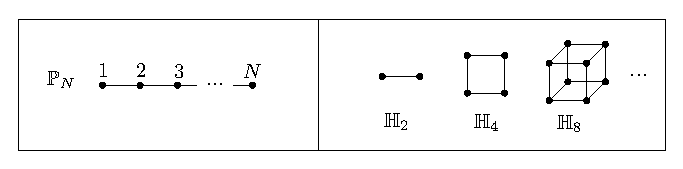
\includegraphics[width=0.78\textwidth]{graphs3.eps}
    \caption{\label{fig:path} The path graph $\graph{P}{N}$ of length $N$ and the first three hypercube graphs $\graph{H}{2}$,$\graph{H}{4}$, and $\graph{H}{8}$.}
  \end{figure}

  In particular, we show that for convex potentials on the path graph $\mathbb{P}_N$ of length $N$ the gap $\Gamma$ is bounded by the gap corresponding to the flat potential
  \begin{equation}
    \Gamma \geq 2\left(1-\cos\left(\frac{\pi}{N}\right)\right).
  \end{equation}
  On the hypercube graph $\graph{H}{2^N}$, for convex potentials dependent only upon vertex Hamming weight, we prove a similar flat-potential lower bound given by
    \begin{equation}
    \Gamma \geq 2.
  \end{equation}

\section{Preliminaries}\label{sec:prelim}
  \subsection{The graph Laplacian and its Eigenvalues}\label{sec:prelim_eigenvalues}
    Let $\mathbb{G}=(V,E)$ be an undirected graph with vertex set $V$ and edge set $E\subseteq V \times V$. Then we associate with $\mathbb{G}$ a degree matrix $\mathbf{D}(\mathbb{G})$ and an adjacency matrix $\mathbf{A}(\mathbb{G})$ where
    \begin{equation}
      \big[\mathbf{D}(\mathbb{G})\big]_{ij} = d_i \delta_{ij}
    \end{equation}
    with $d_i$ the degree of vertex $V_i \in V$ and
    \begin{equation}
      \big[\mathbf{A}(\mathbb{G})\big]_{ij} = \begin{cases}
						1 & \text{if $(V_i,V_j) \in E$} \\
						0 & \text{otherwise}.
					      \end{cases}
    \end{equation}

    One then defines the $\lvert V \rvert \times \lvert V \rvert$ graph Laplacian $\mathbf{L}(\mathbb{G})$ as the difference between the degree matrix and adjacency matrix. That is,
    \begin{equation}
      \mathbf{L}(\mathbb{G}) = \mathbf{D}(\mathbb{G}) - \mathbf{A}(\mathbb{G}).
    \end{equation}

    We now extend our attention to a more general class of Schr\"{o}dinger operators of the form
    \begin{equation}
      \mathbf{H}_W(\mathbb{G}) \stackrel{\text{def}}{=} \mathbf{L}(\mathbb{G}) + \mathbf{W}(V) \label{eqn:hw}
    \end{equation}
    where for some function $W:V\rightarrow\mathbb{R}$, $\mathbf{W}$ is the diagonal matrix defined by
    \begin{equation}
      \big[\mathbf{W}(V)\big]_{ij} \stackrel{\text{def}}{=} W(V_i) \delta_{ij}.
    \end{equation}
    We can think of the resulting matrix as either the graph Laplacian for a weighted graph with loops or as a Schr\"{o}dinger operator (Hamiltonian) with an external potential. The eigenvalue spectrum of $\mathbf{H}_W(\mathbb{G})$ is $\lambda_1 \leq \lambda_2 \leq \dots \leq \lambda_{\size{V}}$ with associated, normalized eigenvectors $\mathbf{u}(\lambda_1),\mathbf{u}(\lambda_2),\dots,\mathbf{u}(\lambda_{\size{V}})$. Suppose now that we consider the one parameter family $\mathbf{H}_W(\mathbb{G};\alpha)$ with
    \begin{equation}
      \mathbf{H}_W(\mathbb{G}) = \mathbf{H}_W(\mathbb{G};\alpha) \Big\rvert_{\alpha=0}.
    \end{equation}
    If $\lambda_k$ is an eigenvalue of $\mathbf{H}_W(\mathbb{G};\alpha)$ with no degeneracy, the Hellman-Feynman theorem governs the relationship between $\lambda_k$ and $\alpha$. That is,
    \HellmanFeynman*

    Our primary interest in this paper is the so-called Fundamental Gap,
    \begin{equation}
      \Gamma(\alpha) \stackrel{\text{def}}{=} \lambda_2(\alpha) - \lambda_1(\alpha)
    \end{equation}
    the difference between the two lowest eigenvalues of $\mathbf{H}_W(\mathbb{G};\alpha)$. Assuming that both $\lambda_1$ and $\lambda_2$ are non-degenerate eigenvalues, by \Cref{thm:Hellman-Feynman} we have that
    \begin{equation}\label{eqn:Hellman-Feynman}
      \frac{d \Gamma(\alpha)}{d \alpha} = \expected{\frac{d \mathbf{H}_W(\mathbb{G};\alpha)}{d \alpha}}{\mathbf{u}(\lambda_2)} - \; \expected{\frac{d \mathbf{H}_W(\mathbb{G};\alpha)}{d \alpha}}{\mathbf{u}(\lambda_1)}
    \end{equation}
    where if we consider $\mathbf{H}_W(\mathbb{G};\alpha) = \mathbf{H}_{\alpha W}(\mathbb{G})$,
    \begin{equation}
      \frac{d \Gamma(\alpha)}{d \alpha} = \expected{\mathbf{W}}{\mathbf{u}(\lambda_2)} - \expected{\mathbf{W}}{\mathbf{u}(\lambda_1)}.
    \end{equation}
 %   Further, since we are interested in lower bounds to the fundamental gap, for a set of potentials, $\mathcal{W}$ we introduce the notation $\varGamma_\mathcal{W}$ to denote the smallest gap from that set.

  \subsection{Eigenvectors of $\mathbf{H}_W(\mathbb{G})$}
    In deriving bounds for $\Gamma$ we make extensive use of the recurrence relations satisfied by the eigenvectors of $\mathbf{H}_W(\mathbb{G})$. Expressing the eigenvalue equation
    \begin{equation}
      \mathbf{H}_W(\mathbb{G}) \mathbf{u}(\lambda) - \lambda \mathbf{u}(\lambda)=0
    \end{equation}
    componentwise, we obtain the following set of linear equations.
    \begin{equation}\label{eqn:recurrence_graph}
      (d_i + W_i - \lambda)u_i(\lambda) = \sum_{(V_i,V_j)\in E} u_j(\lambda) \;\; \text{for $V_i \in V$}
    \end{equation}
    where for simplicity we let $W_i = W(V_i)$.

    When $\mathbb{G}$ is the path graph, we always consider the labeling of $V$ such that $(V_i,V_j) \in E \implies j = i\pm1$. Then, \cref{eqn:recurrence_graph} reduces to
    \begin{equation}\label{eqn:recurrence}
      (2 + W_i - \lambda)u_i(\lambda) = u_{i-1}(\lambda) + u_{i+1}(\lambda) \;\; \text{for $V_i \in V$.}
    \end{equation}
    Here, to simplify the treatment, we introduce fictitious vertices $u_0(\lambda)$ and $u_{\size{V}+1}(\lambda)$. We correspondingly set $u_0(\lambda)=u_1(\lambda)$ and $u_{\size{V}+1}(\lambda)=u_{\size{V}}(\lambda)$ for the path graph.

    For our purposes, it is often convenient to express \cref{eqn:recurrence} in terms of difference equations. For this, we need the forward difference operator.
    \begin{definition}[Forward Difference Operator]\label{def:forward_difference}
      For a given sequence $\left(u_i\right)$, we define $\Delta$, the forward difference operator, by $\Delta u_i = u_{i+1} - u_i$. We further define $\Delta^2$, the second difference operator, by $\Delta^2 u_i = u_{i+1} - 2 u_i + u_{i-1}$.
    \end{definition}
       It is also useful to note that for any sequence $(u_i)$,
      \begin{equation}\label{eqn:forward_sum}
	\sum_{i=a}^b \Delta u_i = u_{b+1} - u_a.
      \end{equation}

    \begin{remark}
      The reader should note that our notation yields $\Delta \left(\Delta u_i \right) \neq \Delta^2 u_i$. This makes $\Delta^2$ a central difference operator, not a forward difference operator. This choice is convenient, since it allows us to easily keep track of indices as seen below in \cref{eqn:recurrence_difference}.
    \end{remark}

    Now, applying \Cref{def:forward_difference}, \cref{eqn:recurrence} becomes
    \begin{equation}\label{eqn:recurrence_difference}
      \Delta^2 u_i(\lambda) = (W_i - \lambda) u_i(\lambda)
    \end{equation}
    which, similar to the second derivative of a continuous function, is an expression of the convexity of $\mathbf{u}$ at $u_i$.

    We now define some other useful properties of sequences, which we will apply to both sequences and vectors without restatement.
    \begin{definition}[Generalized Zero]\label{def:generalized_zero}
      For a given sequence $\left(u_i\right)$ we call $u_m \in \left(u_i\right)$ a generalized zero if $u_m u_{m+1} < 0$ or $u_m = 0$.
    \end{definition}
    \begin{definition}
      For a given sequence $(u_i)$ we call the piecewise linear curve connecting Cartesian coordinates $(i,u_i)$ the $\mathbf{u}$-line.
    \end{definition}
    \begin{definition}\label{def:node}
      For a given sequence $(u_i)$ we call a point at which the $\mathbf{u}-line$ intersects zero a node and label it by its $x$-coordinate. From \Cref{def:generalized_zero} if $u_m \in (u_i)$ is a generalized zero, then the $\mathbf{u}$-line has a node at $x$ with $x\in[m,m+1)$.
    \end{definition}

    For two sequences $(u_i),(v_i)$ we will frequently need the discrete analogue of the Wronskian, the Casoratian sequence $(w_i)$. Suppose that $\mathbf{u}(\mu;\beta),\mathbf{u}(\lambda;\alpha)$ are two sequences (vectors) with $\mu > \lambda$, satisfying \cref{eqn:recurrence}, and parameterized by $\beta$ and $\alpha$ respectively. Then, we are interested in
    \begin{equation}
      w_i\big(\mathbf{u}(\mu;\beta),\mathbf{u}(\lambda;\alpha)\big) = u_{i+1}(\mu;\beta)u_i(\lambda;\alpha) - u_i(\mu;\beta)u_{i+1}(\lambda;\alpha)
    \end{equation}
    which, when applied to \cref{eqn:recurrence} yields
    \begin{equation}\label{eqn:Casoratian}
      \Delta w_{i-1}\big(\mathbf{u}(\mu;\beta),\mathbf{u}(\lambda;\alpha)\big) = \Theta_{W,i}(\mu-\lambda;\beta,\alpha) u_{i}(\mu;\beta)u_i(\lambda;\alpha)
    \end{equation}
    where
    \begin{equation}\label{eqn:theta}
      \Theta_{W,i}(\gamma;\beta,\alpha) \stackrel{\text{def}}{=} W_i(\beta) - W_i(\alpha) - \gamma.
    \end{equation}

\section{The Path Graph $\mathbb{P}_{N}$}\label{sec:path}

  For the path graph $\mathbb{P}_N$ depicted in \Cref{fig:path}, we are interested in the case of convex potentials, for which we offer the following definition:
    \begin{definition}\label{def:convex}
      Let $\intset{a}{b} = \{a,a+1,\dots,b-1,b\}$. Let $\mathbb{P}_N$ be the path graph with vertex set $V=\{V_i\}_{i\in \intset{1}{N}}$ and edge set $E=\big\{(V_i,V_{i+1})\big\}_{i\in\intset{1}{N-1}}$. Let $\mathcal{W}$ be the set of all convex functions $w:\mathbb{R}\rightarrow\mathbb{R}$. We call $W:V\rightarrow \mathbb{R}$ convex if there exists some $w \in \mathcal{W}$ such that $W(V_i) = w(i) \; \forall \; V_i \in V$.

      We similarly define the term ``linear'' and denote its set $\mathcal{L}$.
    \end{definition}

  We begin by using variational arguments to demonstrate that the gap corresponding to each $W\in\mathcal{W}$ is bounded from below by the gap corresponding to some $L\in\mathcal{L}$. This approach is modeled on that used by Lavine in the continuum.\cite{Lavine1994} Then, we use the geometry of the eigenvectors of $\mathbf{H}_L(\mathbb{P}_N)$ to demonstrate that the gap of each linear potential $L$ is bounded from below by the gap for a constant potential.

  \subsection{The gap for convex potentials is lower bounded by the gap for linear potentials.}
  The eigenvalues of $\mathbf{H}_W(\mathbb{P}_N)$ are real and ordered $\lambda_1 < \lambda_2 < \dots < \lambda_N$. Also, recall that we have introduced fictitious points $u_0(\lambda)$ and $u_{N+1}(\lambda)$ to satisfy the recurrence \cref{eqn:recurrence}. Then we have the following fact about the intersections of the $\mathbf{u}(\lambda_1)$-line and $\mathbf{u}(\lambda_2)$-line.
  \begin{lem}\label{lem:intersection}
    Let $0\leq\lambda_1<\lambda_2$ be the two lowest eigenvalues of $\mathbf{H}_{W}(\mathbb{P}_N)$ for convex $W$, and let $\mathbf{u}(\lambda_1),\mathbf{u}(\lambda_2)$ be their corresponding eigenvectors. Then, $\exists m<n \in \intset{1}{N}$ such that $u_{i}^2(\lambda_2) - u_{i}^2(\lambda_1) \geq 0$ for all $i \in \intset{1}{m}\cup\intset{n+1}{N}$ and $u_{i}^2(\lambda_2) - u_{i}^2(\lambda_1) < 0$ for all $i \in \intset{m+1}{n}$.
  \end{lem}
  \begin{proof}
    The intersections of $\mathbf{u}(\lambda_1)$ and $\mathbf{u}(\lambda_2)$ can be characterized by the behavior of the quantity
    \begin{align}
      \Delta\left(\frac{u_i(\lambda_2)}{u_i(\lambda_1)} \right) &= \frac{u_{i+1}(\lambda_2)u_i(\lambda_1)-u_i(\lambda_2)u_{i+1}(\lambda_1)}{u_{i+1}(\lambda_1)u_i(\lambda_1)} \\
								&\equiv \frac{w_i\big(\mathbf{u}(\lambda_2),\mathbf{u}(\lambda_1)\big)}{u_{i+1}(\lambda_1)u_i(\lambda_1)}. \label{eq:cas_temp}
    \end{align}

    For simplicity, let $w_i = w_i\big(\mathbf{u}(\lambda_2),\mathbf{u}(\lambda_1)\big)$. Then, in \cref{eqn:Casoratian} we can set $\alpha=\beta=0$, yielding
    \begin{equation}\label{eqn:Casoratian_diff}
      \Delta w_{i-1} = -\Gamma u_i(\lambda_2)u_i(\lambda_1)
    \end{equation}
    and since $u_0(\cdot) = u_1(\cdot)$ and $u_N(\cdot) = u_{N+1}(\cdot)$, $w_{0}=w_{N}=0$. Thus, from \cref{eqn:forward_sum,eqn:Casoratian_diff} we have
    \begin{align}
      w_n &= w_0 + \sum_{i=0}^{n-1}\Delta w_i \\
	  &= -\Gamma \sum_{i=0}^{n-1}u_{i+1}(\lambda_2)u_{i+1}(\lambda_1) \label{eqn:cas_up} \\
	  &= \Gamma \sum_{i=n}^{N-1}u_{i+1}(\lambda_2)u_{i+1}(\lambda_1) \label{eqn:cas_down}.
    \end{align}
    Here, because $\mathbf{H}_W(\mathbb{P}_N)$ is a Jacobi matrix, we are free to choose $\mathbf{u}(\lambda_1)$ as everywhere positive and $\mathbf{u}(\lambda_2)$ as initially positive with no loss of generality. Further, it is known that $\mathbf{u}(\lambda_1)$ has no generalized zeros and $\mathbf{u}(\lambda_2)$ has exactly one, which we identify with $u_{\sigma}(\lambda_2)$. (See \textit{e.g.} Gantmakher.\cite{gantmakher2002oscillation}) Then, from \cref{eqn:cas_up}
    \begin{eqnarray}
      w_{n\leq \sigma} &=& -\Gamma \sum_{i=0}^{n-1}u_{i+1}(\lambda_2)u_{i+1}(\lambda_1) \\
		  &\leq& 0
    \end{eqnarray}

    Similarly, from \cref{eqn:cas_down}
    \begin{eqnarray}
      w_{n > \sigma} &=& \Gamma \sum_{i=n}^{N-1}u_{i+1}(\lambda_2)u_{i+1}(\lambda_1) \\
		&\leq& 0
    \end{eqnarray}
    so that we have $w_n \leq 0 \; \forall \; n \in \intset{0}{N}$.

    Finally, by \cref{eq:cas_temp} we arrive at
    \begin{equation}
      \Delta\left(\frac{u_i(\lambda_2)}{u_i(\lambda_1)} \right)\leq 0 \; \forall \; i \in \intset{0}{N}.
    \end{equation}
    Now, this sequence can be divided into three regions, where we will find that at least two of these regions are nonempty. Specifically, that this quantity is always decreasing guarantees that there exists some choice of $m < n \in \intset{1}{N}$ such that
    \begin{equation}\label{eqn:regions}
      \begin{cases}
    	\left(\frac{u_i(\lambda_2)}{u_i(\lambda_1)} \right) > 1, & i \in \intset{1}{m} \\
    	-1 \leq \left(\frac{u_i(\lambda_2)}{u_i(\lambda_1)} \right) \leq 1, & i \in \intset{m+1}{n} \\
    	\left(\frac{u_i(\lambda_2)}{u_i(\lambda_1)} \right) < -1, & i \in \intset{n+1}{N}
      \end{cases}
    \end{equation}
    and hence $\big(u_{i}^2(\lambda_2) - u_{i}^2(\lambda_1)\big)_{i=1}^N$ has at most two generalized zeros. Further, that $u_{i}(\lambda_2),u_{i}(\lambda_1)$ are normalized and orthogonal eigenvectors guarantees that $\big(u_{i}^2(\lambda_2) - u_{i}^2(\lambda_1)\big)_{i=1}^N$ has at least one generalized zero. Thus, our proof is complete.
  \end{proof}

  Using \Cref{lem:intersection} we now prove a discrete analogue of Lemma 3.2 from Lavine\cite{Lavine1994}:
  \begin{lem}\label{lem:lavine}
	Let $\mathcal{W}$ be the set of convex potentials and $\mathcal{L}\subseteq{\mathcal{W}}$ be the set of linear potentials. Let $\mathbf{u}(\lambda_1)$, $\mathbf{u}(\lambda_2)$ be the two lowest eigenvectors of some $\mathbf{H}_{W}(\mathbb{P}_N)$ satisfying \cref{eqn:regions}.  Then, $\forall \;W\in\mathcal{W} \; \exists L \in \mathcal{L} \;\rvert\; \Gamma(\mathbf{H}_{W}(\mathbb{P}_N)) \geq \Gamma(\mathbf{H}_{L}(\mathbb{P}_N))$.
  \end{lem}

  \begin{proof}
  	 Identify with $W(V_i)$ a convex function $w: \mathbb{R} \rightarrow \mathbb{R}$ such that $w(i)=W(V_i) \; \forall \; i \in \intset{1}{N}$. Then, we define the linear function $l_w: \mathbb{R} \rightarrow \mathbb{R}$ as
  	\begin{eqnarray}
  		l_w(i) = \frac{1}{n-m}\bigg((n-i)w(m) + (i-m)w(n)\bigg)
  	\end{eqnarray}
  	with $n$ and $m$ defined as in \Cref{lem:intersection}, and identify it with the corresponding $L_W \in \mathcal{L}$. Notably, $L_W(V_i) \leq W(V_i) \; \forall \; i \in \intset{1}{m}\cup\intset{n+1}{N}$ and $L(V_i) \geq W(V_i) \; \forall \; i \in \intset{m+1}{n}$. Then, clearly
	\begin{equation}
	  \langle\mathbf{W}-\mathbf{L}_W\rangle_{\mathbf{u}(\lambda_2)} - \langle\mathbf{W}-\mathbf{L}_W\rangle_{\mathbf{u}(\lambda_1)} \geq 0 \label{eq:39}
	\end{equation}
	where equality is obtained only when $W=L_W$.

	Now we consider the Schr\"{o}dinger operator that satisfies
	\begin{equation}
		\mathbf{H}_{W}(\mathbb{P}_N;\alpha) = \mathbf{H}_{W(\alpha)}(\mathbb{P}_N)
	\end{equation}
	and identify with $W(\alpha)$ the convex function $w(i;\alpha)$
	\begin{eqnarray}
		w(i;0) &=& w(i) \\
		\frac{d{w}}{d \alpha}(i;\alpha) &=& l_{w(\cdot;\alpha)}(i) - w(i;\alpha).
	\end{eqnarray}
	Thus, by \cref{eqn:Hellman-Feynman,eq:39} we have that the gap of $\mathbf{H}_{W(\alpha)}(\mathbb{P}_N)$ decreases with $\alpha$ and additionally that
	\begin{equation}\label{eqn:converge}
		w(i;\alpha) = e^{-\alpha}w(i) + \int_0^\alpha \frac{e^{s-\alpha}}{n(s)-m(s)}\bigg((n(s)-i)w\big(m(s);s\big) + (i-m(s))w\big(n(s);s\big)\bigg)ds.
	\end{equation}
	Hence, as $\alpha$ increases, we have that $w(i;\alpha)$ gets arbitrarily close to a linear function and therefore $W(\alpha)$ gets arbitrarily close to some function in $\mathcal{L}$.
  \end{proof}

  \subsection{The gap for linear potentials is lower bounded by the gap for constant potentials.}
    We start with $\mathbf{u}(\lambda_2),\mathbf{u}(\lambda_1)$ as the eigenvectors of $\mathbf{H}_{W}(\mathbb{P}_N)$ for some $W \in \mathcal{W}$. By \Cref{lem:lavine} we need only demonstrate that gaps associated with the class of linear potentials are lower bounded by the gaps associated with the constant potential. Because we are confined to a discrete setting, this takes a bit of work. The overall strategy is as follows: First, we restrict ourselves to a particular class of linear potentials and demonstrate that $\mathbf{u}(\lambda_1)$ is strictly decreasing. Then, we prove some facts about the ordering of the components of $\mathbf{u}(\lambda_2)$ around its node. Next, we demonstrate that for positive slopes, $\mathbf{u}(\lambda_2)$ always has a node left of center. These facts combine to complete our proof.

    We introduce the notation $\left[\mathbf{U}\right]_{ij} = (i-1)\delta_{ij}$ for the unit linear potential. Note that for any linear potential $L \in \mathcal{L}$ with slope $\alpha$, the potential $\alpha U$ has the same gap. Thus, we restrict our study to the unit potential multiplied by some parameter $\alpha$. Further, symmetry allows us to restrict ourselves to the case that $\alpha\geq0$.

    Our goal is to demonstrate that
    \begin{equation}\label{eqn:goal}
    	\frac{d \Gamma(\alpha)}{d \alpha} > 0
    \end{equation}
    for all $\alpha \geq 0$.

    We make use of the following lemma to reduce to the case that $u_1^2(\lambda_2) > u_1^2(\lambda_1)$:
    \begin{lem}\label{lem:simplify}
    	Let $\alpha U\in\mathcal{L}$ where $U$ is the unit-linear potential. Then, for $\mathbf{H}_{\alpha U}(\mathbb{P}_N)$, if $u_1^2(\lambda_2) \leq u_1^2(\lambda_1)$, \cref{eqn:goal} is satisfied.
    \end{lem}

    \begin{proof}
      By \cref{eqn:Hellman-Feynman},
      \begin{align}
      	\frac{d\Gamma(\alpha)}{d \alpha} &= \sum_{i=1}^{N}\left(u_i^2(\lambda_2)-u_i^2(\lambda_1)\right) (i-1)  \\
      	&= \sum_{i=1}^{N}\left(u_i^2(\lambda_2)-u_i^2(\lambda_1)\right) (i - c) \label{eqn:bla}
      \end{align}
      for any constant $c$. (Recall that the $\mathbf{u}(\lambda)$ are normalized eigenvectors.) From \Cref{lem:intersection} we know that if $u_1^2(\lambda_2) \leq u_1^2(\lambda_1)$ then $\exists n < N$ such that $u_i^2(\lambda_2)-u_i^2(\lambda_1) > 0$ for all $i>n$. Choosing $c = n$ we get that eq. (\ref{eqn:bla}) is non-negative for each term of the sum, thus completing the proof.
    \end{proof}

    Having reduced to the case that $u_1^2(\lambda_2) \geq u_1^2(\lambda_1)$, we now prove that $\mathbf{u}(\lambda_1)$ is a decreasing sequence:

    \begin{lem}\label{lem:decreasing}
    	Let $\mathbf{H}_{\alpha U}(\mathbb{P}_N)$ be defined as in \Cref{lem:simplify}. Then, $\mathbf{u}(\lambda_1)$ is a decreasing sequence. Further, for $\alpha > 0$, $\mathbf{u}(\lambda_1)$ is strictly decreasing.
    \end{lem}

    \begin{proof}
    First we note that at the boundaries, $\Delta u_0(\lambda_1) = \Delta u_N(\lambda_1) = 0$. Thus we know that the boundaries are local extrema of the $\mathbf{u}(\lambda_1)$-line. Now, we note that by \cref{eqn:recurrence}
    \begin{equation}
      \frac{u_2(\lambda_1)}{u_1(\lambda_1)} = (1 - \lambda_1) \leq 1
    \end{equation}
    where the inequality is strict for $\alpha > 0$ since this requires that $\lambda_1 > 0$. Thus, the $\mathbf{u}(\lambda_1)$-line is initially decreasing. Note that from \cref{eqn:recurrence_difference} when $\mathbf{W} = \mathbf{U}$, $\Delta^2 u_i(\lambda_1)$ has at most one sign change. Thus, the second boundary term cannot be a maximum and, therefore, both boundaries must be global extrema. We therefore have that $\mathbf{u}(\lambda_1)$ is decreasing for $\alpha \geq 0$ and strictly decreasing for $\alpha > 0$.
    \end{proof}

    We now recall a theorem by Cauchy and use it to derive an upper bound for $\lambda_2$:
    \begin{thm}[Cauchy Interlace Theorem]\label{thm:Cauchy}
    	Let $\mathbf{A}$ be an $N\times N$ Hermitian matrix with eigenvalues $\lambda_1 \leq \lambda_2 \leq \dots \leq \lambda_N$. Suppose that B is an $(N-1)\times (N-1)$ principal submatrix of $\mathbf{A}$ with eigenvalues $\mu_1 \leq \mu_2 \leq \dots \leq \mu_{N-1}$. Then, the eigenvalues are ordered such that $\lambda_1 \leq \mu_1 \leq \lambda_2 \leq \mu_2 \leq \dots \leq \lambda_{N-1} \leq \mu_{N-1} \leq \lambda_N$.
    \end{thm}
    \begin{proof}
      For proof, we refer the reader to Hwang. \cite{Hwang2004}
    \end{proof}
    \begin{lem}\label{lem:upper}
    	Suppose that an $N \times N$ Hermitian matrix $\mathbf{A}$ with $N \geq 3$ has the $3\times 3$ principal submatrix
    	\[\mathbf{B}(\delta) = \left( \begin{array}{ccc}
	2 - \delta & -1 & 0 \\
	-1 & 2 + \alpha & -1 \\
	0 & -1 & 2 + 2\alpha
    	\end{array} \right) \]
    	with $\delta \geq 0$. Then, if $\lambda_2$ is the second lowest eigenvalue of $\mathbf{A}$, $\lambda_2 \leq 2 + \alpha$.
    \end{lem}
    \begin{proof}
    	Let $\mu_1(\delta) \leq \mu_2(\delta) \leq \mu_3(\delta)$ be the eigenvalues of $\mathbf{B}(\delta)$. That $\lambda_2 \leq \mu_2(\delta)$ is obvious from repeated applications of \Cref{thm:Cauchy}. From, \Cref{thm:Hellman-Feynman},
    	\begin{equation}
    		\frac{d \mu_2(\delta)}{d \delta} \leq 0
    	\end{equation}
    	and by direct calculation, $\mu_2(0) = 2 + \alpha$. Thus, $\lambda_2 \leq 2 + \alpha$.
    \end{proof}

    \Cref{lem:upper} now combines with the following fact to give an ordering of the components of $\mathbf{u}(\lambda_2)$:
    \begin{lem}\label{lem:convex_combinations}
    	Let $\mathbf{H}_{\alpha U}(\mathbb{P}_N)$ be defined as in \cref{lem:simplify} and let $\mathbf{u}(\lambda)$ be an eigenvector. Define the quantity
    	\begin{equation}\label{def:convex_combinations}
    		u_{i+\epsilon}(\lambda) \stackrel{\text{def}}{=} \epsilon u_{i+1}(\lambda) + (1-\epsilon)u_{i}(\lambda).
    	\end{equation}
	Then, for $u_{i}(\lambda)$ not a generalized zero,
	\begin{equation}\label{eqn:recurrence_cc}
	  u_{i+1+\epsilon}(\lambda) = \left(2+\alpha(j_{i+\epsilon}-1)-\lambda\right)u_{i+\epsilon} - u_{i-1+\epsilon}
	\end{equation}
	for some $j_{i+\epsilon} \in \left[i,i+1\right]$.
    \end{lem}
    \begin{proof}
    	First, note that from \cref{eqn:recurrence}
    	\begin{equation}\label{eqn:cc_1}
    		u_{i+1+\epsilon}(\lambda) = \left(2-\lambda\right)u_{i+\epsilon}(\lambda) + \alpha \left(i \epsilon u_{i+1}(\lambda) + (i-1)(1-\epsilon)u_{i}(\lambda) \right) -  u_{i-1+\epsilon}(\lambda).
    	\end{equation}
	Now, with $\text{sign}(u_{i+1}(\lambda))=\text{sign}(u_i(\lambda))$, there exists a $j_{i+\epsilon} \in \left[i,i+1\right]$ such that
	\begin{equation}
		i \epsilon u_{i+1}(\lambda) + (i-1)(1-\epsilon)u_{i}(\lambda) = (j_{i+\epsilon}-1) \left(\epsilon u_{i+1}(\lambda) + (1-\epsilon)u_{i}(\lambda)\right).
	\end{equation}
	Thus, \cref{eqn:cc_1} becomes
	\begin{equation}
    		u_{i+1+\epsilon}(\lambda) = \left(2+\alpha (j_{i+\epsilon}-1) -\lambda\right)u_{i+\epsilon}(\lambda) -  u_{i-1+\epsilon}(\lambda).
    	\end{equation}
    \end{proof}
    \begin{lem}[Ordering $\mathbf{u}(\lambda_2)$]\label{lem:ordering_2}
    	Let $\mathbf{H}_{\alpha U}(\mathbb{P}_N)$ be defined as in \Cref{lem:simplify}. Let $x$ represent the first node of the $\mathbf{u}(\lambda_2)$-line and let $u_m(\lambda_2)$ be the corresponding generalized zero. Suppose that $x \leq (N+1)/2$. Let $u_{i+\epsilon}(\lambda)$ be defined as in \Cref{lem:convex_combinations}. Then,
    	\begin{equation}
	-1 \geq \begin{cases}
 			\frac{u_{m+k+\epsilon}(\lambda_2)}{u_{m-1-k+\epsilon}(\lambda_2)} \; \; \text{for $m \leq x \leq m + \frac{1}{2}$ and $k \in \intset{0}{m-1}$} \\
 			\frac{u_{m+k+\epsilon}(\lambda_2)}{u_{m-k+\epsilon}(\lambda_2)} \; \; \text{for $m + \frac{1}{2} < x \leq m + 1$ and $k \in \intset{1}{m}$}.
 		\end{cases}
 	\end{equation}
    \end{lem}

    \begin{proof}
      We proceed to prove this lemma by induction. First, consider the case that $m+1/2 \leq x < m+1$ for some $m\in \intset{1}{\lfloor N/2 \rfloor}$. For simplicity, let $\mathbf{u}(\lambda_2) = \mathbf{u}$. Then, there exists an $\epsilon$ such that $(1-\epsilon)u_{m}+\epsilon u_{m+1}=0$. So, from \cref{eqn:cc_1} we can consider the base case
      \begin{align}\label{eqn:base_1}
	u_{m+1+\epsilon} &= \epsilon \alpha u_{m+1} - u_{m-1+\epsilon} \\
	&< -u_{m-1+\epsilon}.
      \end{align}
      For the induction, rearrange \cref{eqn:recurrence_cc} for terms left and right of the node,
      \begin{equation}\label{eqn:temp6}
      	\frac{u_{m+k+2+\epsilon}+u_{m+k+\epsilon}}{u_{m+k+1+\epsilon}} - \frac{u_{m-k-2+\epsilon}+u_{m-k+\epsilon}}{u_{m-k-1+\epsilon}} = \alpha(j_{m+k+1+\epsilon}-j_{m-k-1+\epsilon}) > 0.
      \end{equation}
      Now assume
      \begin{equation}\label{eqn:assumption}
      	\frac{u_{m+k+\epsilon}}{u_{m+k+1+\epsilon}} \leq \frac{u_{m-k+\epsilon}}{u_{m-k-1+\epsilon}}
      \end{equation}
      thus, by \cref{eqn:temp6}
      \begin{equation}
      	\frac{u_{m+k+2+\epsilon}}{u_{m+k+1+\epsilon}} \geq \frac{u_{m-k-2+\epsilon}}{u_{m-k-1+\epsilon}}.
      \end{equation}
      Thus,
      \begin{equation}
      	\frac{u_{m+k+2+\epsilon}}{u_{m-k-2+\epsilon}} \leq \frac{u_{m+k+1+\epsilon}}{u_{m-k-1+\epsilon}}.
      \end{equation}
      Finally, taking $k=0$, \cref{eqn:base_1} satisfies \cref{eqn:assumption} and
      \begin{equation}
      	\frac{u_{m+k'+\epsilon}}{u_{m-k'+\epsilon}} \leq -1
      \end{equation}
      for all $k' \in \intset{1}{m}$.

      Next we consider the case that $m \leq x < m+1/2$. In this case, by \Cref{def:node} we can choose $\epsilon$ such that $u_{m+\epsilon} = -u_{m-1+\epsilon}$. Then,
      \begin{equation}\label{eqn:temp5}
      	\frac{u_{m+k+1+\epsilon}+u_{m+k-1+\epsilon}}{u_{m+k+\epsilon}} - \frac{u_{m-k-2+\epsilon}+u_{m-k+\epsilon}}{u_{m-k-1+\epsilon}} = \alpha(j_{m+k+\epsilon}-j_{m-k-1+\epsilon}) > 0.
      \end{equation}
      This time, assume
      \begin{equation}\label{eqn:assumption_2}
      	\frac{u_{m+k-1+\epsilon}}{u_{m+k+\epsilon}} \leq \frac{u_{m-k+\epsilon}}{u_{m-k-1+\epsilon}}
      \end{equation}
      then, by \cref{eqn:temp5}
      \begin{equation}
      	\frac{u_{m+k+1+\epsilon}}{u_{m+k+\epsilon}} \geq \frac{u_{m-k-2+\epsilon}}{u_{m-k-1+\epsilon}}.
      \end{equation}
      Hence,
      \begin{equation}
      	\frac{u_{m+k+1+\epsilon}}{u_{m-k-2+\epsilon}} \leq \frac{u_{m+k+\epsilon}}{u_{m-k-1+\epsilon}}.
      \end{equation}
      Again, taking $k=0$, we have that
      \begin{equation}
      	\frac{u_{m+k'+\epsilon}}{u_{m-1-k'+\epsilon}} \leq \frac{u_{m+\epsilon}}{u_{m-1+\epsilon}} \leq -1.
      \end{equation}
      for all $k' \in \intset{0}{m-1}$.
    \end{proof}

    Now, we recall a theorem due to Gantmakher and Kre\u{i}n:\cite{gantmakher2002oscillation}
    \begin{restatable}{thm}{Gantmakher}\label{thm:Gantmakher}
      Let $\mathbf{u}(\mu;\alpha)$,$\mathbf{u}(\lambda;\beta)$ be two vectors of length $N$ satisfying \cref{eqn:recurrence} and with
      \begin{equation} \label{eqn:rest}
	      \Theta_{W,i}(\mu-\lambda;\alpha,\beta) \leq 0 \;\; \text{$\forall \; i \in \intset{m}{n}$}
      \end{equation}
      where $\Theta_{W,i}(\mu-\lambda;\alpha,\beta) < 0$ for at least some $i \in \intset{m}{n}$. We extend both vectors to length $N+2$ by including nodes at $u_0$ and $u_{N+1}$. (So long as \cref{eqn:recurrence} is satisfied, despite previous choices of $u_0$ and $u_{N+1}$, these points are always considered nodes.) Let $\eta \in [m-1,m), \xi \in (n,n+1]$ be two adjacent nodes of $\mathbf{u}(\lambda;\beta)$ with $m \leq n \in \intset{0}{N+1}$. Then there exists at least one node of $\mathbf{u}(\mu;\alpha)$ between $\eta$ and $\xi$.
    \end{restatable}
    \begin{proof}
    	This fact is adapted directly from Gantmakher and Kre\u{i}n, with modifications made to allow for our parameterization. The argument is provided in detail in \Cref{app:Gantmakher} for the unfamiliar reader.
    \end{proof}
  \begin{restatable}{lem}{Node}\label{lem:node_left}
%    \begin{lem}\label{lem:node_left}
      Let $\mathbf{H}_{\alpha U}(\mathbb{P}_N)$ be defined as in \Cref{lem:simplify}. $\mathbf{u}(\lambda_2)$ always has a node at or left of $x=(N+1)/2$.
%    \end{lem}
  \end{restatable}
    \begin{proof}
    We only want to consider variations with respect to one parameter, so we fix $\lambda=\mu_0,\alpha=\beta_0$. Then, we note that, by \cref{eqn:theta}, $\Theta_{U,i}$ is an increasing sequence in $i$. Now, we assume that there exists a node of $\mathbf{u}(\mu_0)$ at $x=(N+1)/2$. Next, at $\beta=\beta_0$ and $\mu=\mu_0$, $\Theta_{U,i}$ is identically $0$. Then,
      \begin{equation}\label{eq:theta_vary}
	\frac{d \Theta_{U,i}}{d\beta}\bigg\rvert_{\mu=\mu_0} = U_i - \frac{d \mu}{d \beta}\bigg\rvert_{\mu=\mu_0}= U_i - \langle \mathbf{U} \rangle_{\mathbf{u}(\mu_0)}
      \end{equation}
      Our assumption that $\mathbf{u}(\mu_0)$ at $x=(N+1)/2$ requires that $\epsilon=1$ in \Cref{lem:ordering_2}. Then, \Cref{lem:ordering_2} becomes an exact statement about the ordering of the components of $\mathbf{u}(\mu_0)$. Hence, $\langle \mathbf{U}\rangle_{\mathbf{u}(\mu_0)} \geq (N-1)/2$ and we have that
      \begin{align}\label{eq:node_theta}
	U_{\left\lfloor\frac{N+1}{2}\right\rfloor} - \left\langle \mathbf{U} \right\rangle_{\mathbf{u}(\mu_0)} &\leq U_{\left\lfloor\frac{N+1}{2}\right\rfloor} - \frac{N-1}{2} \\
	&= \left(\left\lfloor\frac{N+1}{2}\right\rfloor - 1\right) - \frac{N-1}{2} \\
	&\leq 0.
      \end{align}
      Further, in the same fashion
      \begin{equation}
      	U_{\left\lfloor\frac{N+1}{2}-1\right\rfloor} - \left\langle \mathbf{U} \right\rangle_{\mathbf{u}(\mu_0)} < 0.
      \end{equation}
      Hence, for some $\beta-\beta_0=\xi>0$ with $\xi$ sufficiently close to 0, $\Theta_{U,i}\leq0 \; \forall \; i \in \intset{1}{\lfloor(N+1)/2\rfloor}$ with at least some $i$ such that $\Theta_{U,i}<0$. Thus, at $\beta=\beta_0$ the node of $\mathbf{u}(\lambda_2)$ shifts left as $\beta$ increases. Note that if $\beta=\beta_0=0$, symmetry forces the node of the $\mathbf{u}(\mu)$-line to occur at $x=(N+1)/2$. Thus, there is initially a node at $(N+1)/2$ and whenever there is a node at $x=(N+1)/2$ it shifts left. Hence, there is always a node at or left of $(N+1)/2$.
    \end{proof}

    \begin{remark}
    	In fact, with some of the facts that follow, we demonstrate that the node shifts left with increasing $\alpha$. For proof, see \Cref{app:Sturm-Picone}.
    \end{remark}

    \Cref{lem:node_left} allows us to strengthen \Cref{lem:ordering_2} through the following fact:
        \begin{lem}\label{lem:decreasing_2}
    	Let $\mathbf{H}_{\alpha U}(\mathbb{P}_N)$ be defined as in \Cref{lem:simplify}. Let $x$ represent the first node of the $\mathbf{u}(\lambda_2)$-line. Then, there exists a symmetric region $S=\intset{1}{m}$ about $x$ such that $\mathbf{u}(\lambda_2)$ is a decreasing sequence.
    \end{lem}

    \begin{proof}
    	We begin by considering the first point after the node such that $\mathbf{u}(\lambda_2)$ is increasing and label it by $m$ such that $\Delta u_m (\lambda_2) \Delta u_{m-1}(\lambda_2) < 0$. Then,
    	\begin{equation}\label{eqn:decreasing_1}
    		u_{m+1}(\lambda_2) = \left(2 + \alpha (m-1) -\lambda_2\right) u_m(\lambda_2) - u_{m-1}(\lambda_2).
    	\end{equation}
    	Now, rearranging \cref{eqn:decreasing_1}
    	\begin{equation}\label{eqn:sub_path}
    		u_m(\lambda_2) = \left(2 + \left(1 - \frac{u_{m+1}(\lambda_2)}{u_{m}(\lambda_2)}\right) +\alpha (m-1) -\lambda_2\right) u_m(\lambda_2)-u_{m-1}(\lambda_2).
    	\end{equation}
    	Note that in \cref{eqn:sub_path}, because $u_m(\lambda_2)\leq u_{m+1}(\lambda_2)<0$, we know that $1 > u_{m+1}(\lambda_2)/u_m(\lambda_2)$ and thus $(u_i(\lambda_2))_{i\in\intset{1}{m}}$ is an eigenvector of  $\mathbf{H}_W(\graph{P}{m})$ where
    	\begin{equation}
	  W_i = \alpha U_i + \delta_{im}\left(1 - \frac{u_{m+1}(\lambda_2)}{u_{m}(\lambda_2)}\right).
	\end{equation}
	By \Cref{lem:node_left} the second eigenvector of $\mathbf{H}_{\alpha U}(\graph{P}{m})$ has a node left of center. Since $\lambda_2$ is greater than the second eigenvalue of $\mathbf{H}_{\alpha U}(\graph{P}{m})$ and we know that $\mathbf{W}$ is identical to $\mathbf{U}$ in all but the $m^{\text{th}}$ component, we have by \Cref{thm:Gantmakher} that $\left(u_i(\lambda_2)\right)_{i\in\intset{1}{m}}$ has a node left of center. Further, by our assumptions, $(u_i(\lambda_2))_{i\in\intset{1}{m}}$ is a decreasing sequence. Therefore, there exists a symmetric region $S=\intset{1}{m}$ about $x$ such that $\mathbf{u}(\lambda_2)$ is strictly decreasing.
    \end{proof}

    Using \Cref{lem:decreasing_2} we now prove a corollary to \Cref{lem:ordering_2} that holds regardless of whether the node falls directly on a vertex:
       \begin{cor}\label{cor:ordering}
    	Let $\mathbf{H}_{\alpha U}(\mathbb{P}_N)$ and $x$ be defined as in \cref{lem:ordering_2}. Let $\mathbf{u}(\lambda_2)$ be a decreasing sequence. Then,
    	\begin{equation}
	-1 \geq \begin{cases}
 			\frac{u_{m+k+1}(\lambda_2)}{u_{m-k}(\lambda_2)} \; \; \text{for $m \leq x \leq m + \frac{1}{2} \forall k \in \intset{0}{m-1}$} \\
 			\frac{u_{m+2+k}(\lambda_2)}{u_{m-k}(\lambda_2)} \; \; \text{for $m + \frac{1}{2} < x \leq m + 1 \forall k \in \intset{1}{m}$}.
 		\end{cases}
 	\end{equation}
    \end{cor}
    \begin{proof}
    	For the first case, assume that $m+1/2 \leq x < m+1$ for some $m\in \intset{1}{\lfloor N/2 \rfloor}$. Then, from \Cref{lem:ordering_2} we have that
    	\begin{equation}
    		-1 \geq \frac{u_{m+k+\epsilon}(\lambda_2)}{u_{m-k+\epsilon}(\lambda_2)} \; \; \text{for $m + \frac{1}{2} < x \leq m + 1 \forall k \in \intset{1}{m}$}.
    	\end{equation}
	Then, since $\mathbf{u}(\lambda_2)$ is decreasing, $u_{m+1+k} \leq u_{m+k+\epsilon}$ and also $u_{m-k+\epsilon} \geq u_{m+1-k}$. Thus,
	\begin{equation}
		-1 \geq \frac{u_{m+k+\epsilon}(\lambda_2)}{u_{m-k+\epsilon}(\lambda_2)} \geq \frac{u_{m+1+k}(\lambda_2)}{u_{m+1-k}(\lambda_2)}.
	\end{equation}

	Similarly, for the case that $m \leq x < m+1/2$, we have that
	\begin{equation}
    		-1 \geq \frac{u_{m+k+\epsilon}(\lambda_2)}{u_{m-1-k+\epsilon}(\lambda_2)} \; \; \text{for $m \leq x \leq m + \frac{1}{2} \forall k \in \intset{1}{m-1}$}.
    	\end{equation}
	In this case, we have that $u_{m-1-k+\epsilon} \geq u_{m-k}$. So that finally,
	\begin{equation}
    		-1 \geq \frac{u_{m+k+\epsilon}(\lambda_2)}{u_{m-1-k+\epsilon}(\lambda_2)} \geq \frac{u_{m+1+k}(\lambda_2)}{u_{m-k}(\lambda_2)}.
    	\end{equation}
    \end{proof}

    \begin{thm}
      For $\mathbb{P}_N$,
      \begin{equation}
      	\Gamma_{W \in \mathcal{W}} \geq 2\left(1-\cos\left(\frac{\pi}{N}\right)\right).
      \end{equation}
    \end{thm}

    \begin{proof}
      From \Cref{thm:Hellman-Feynman} we know that so long as $\langle \mathbf{U} \rangle_{\mathbf{u}(\lambda_2)} - \langle \mathbf{U} \rangle_{\mathbf{u}(\lambda_1)} > 0$, the gap is increasing.

      Consider a set of indices $S_m$ symmetric about $m$, the index corresponding to the first generalized zero $u_m(\lambda_2)$ of $\mathbf{u}(\lambda_2)$. Now, define $\mathbf{v}(\lambda_i) = \big(u(\lambda_i)\big)_{i\in S_m}$. From \Cref{lem:decreasing,lem:ordering_2} we know that
      \begin{equation}
      	\big\langle \mathbf{U} \big\rangle_{\mathbf{v}(\lambda_2)} \geq \big\langle \mathbf{U} \big\rangle_{\mathbf{v}(\lambda_1)}.
      \end{equation}
      where we restrict $\mathbf{U}$ to the same number of terms as $\mathbf{v}(\lambda_2)$.
      By \Cref{lem:node_left} we know that the node of the $\mathbf{u}(\lambda_2)$-line must occur at or before the midpoint of $\mathbf{u}(\lambda_2)$. Thus, $S_m$ can be taken as $S_m = \intset{1}{2m+1}$. By \Cref{lem:simplify} we restrict ourselves to the case that $u_1^2(\lambda_2) > u_1^2(\lambda_1)$. With this restriction, \Cref{lem:ordering_2,lem:decreasing} insist that $u_k^2(\lambda_2) > u_k^2(\lambda_1) \; \forall k \in \intset{1}{N}/S_m$. It is then obvious that
      \begin{equation}
      	\big\langle \mathbf{U} \big\rangle_{\mathbf{u}(\lambda_2)} \geq \big\langle \mathbf{U} \big\rangle_{\mathbf{u}(\lambda_1)}
      \end{equation}
      for $\alpha \geq 0$. Thus, we know that $\Gamma$ is at a minimum for $\alpha=0$. Now, at $\alpha=0$ we find that $\lambda_1=0$ and thus $\Gamma = \lambda_2$. Hence,
      \begin{equation}
	\Gamma_{W \in \mathcal{W}} \geq 2\left(1-\cos\left(\frac{\pi}{N}\right)\right).
      \end{equation}
    \end{proof}

    \section{The Hypercube Graph}
    In this section we find a tight lower bound for the gap for Hamming-symmetric convex potentials on the N-dimensional hypercube graph $\graph{H}{2^N} = (V,E)$. To define $\graph{H}{2^N}$, we identify with each vertex $V_i \in V$ a unique vector $\mathbf{b}_i \in \{0,1\}^N$. Then, we choose $E = \{(V_i,V_j)\; \big\rvert \;|\mathbf{v}_i-\mathbf{v}_j| = 1 \}$, where $|\cdot|$ here denotes the 1-norm. (In the language of computer science, $\mathbf{b}_i, \mathbf{b}_j$ are bit-strings and $|\mathbf{b}_i - \mathbf{b}_j|$ is their Hamming distance.) As in (\ref{eqn:hw}) the Schr\"{o}dinger operator includes a potential term $\mathbf{W}$. Thus, an eigenvector $u(\lambda)$ of eigenvalue $\lambda$ satisfies
    \begin{equation}\label{eqn:recurrence_hyper_prior}
    	(N + W_i - \lambda)u_i(\lambda) = \sum_{(V_i,V_j)\in E} u_j(\lambda) \;\; \text{for $V_i \in V$.}
    \end{equation}
    Here we restrict our attention to the case that the potential depends only on Hamming distance from the vertex of minimum potential. We can label this minimum by the all zeros string, and therefore $W_i = W_{|b_i|}$. In this case, the set of Hamming-symmetric vectors are an invariant subspace of the Schr\"{o}dinger operator.
    \begin{remark}
    In the language of quantum-mechanics, this is the space spanned by the $N+1$ state vectors that are uniform superpositions over bit-strings of a given Hamming weight. By Schr{\"o}dinger's equation, no time-evolution induced by a (possibly time-dependent) Hamming symmetric Hamiltonian will ever drive transitions out of this subspace. For many cases, it is only the gap within this subspace that is of interest.
    \end{remark}
    Below, we will bound the gap within the Hamming-symmetric subspace. Here, the (normalized) uniform superpositions over bit-strings of each Hamming weight form an orthonormal basis for this subspace.    Given a state-vector $\mathbf{u}(\lambda)$, let $v_m(\lambda)$ denote the inner product of $\mathbf{u}(\lambda)$ with the Hamming-weight-$m$ basis vector. That is,
    \begin{equation}
    	v_m(\lambda) = \frac{1}{\sqrt{\binom{N}{m}}} \sum_{|b_i|=m} u_i(\lambda).
    \end{equation}

    Because $\mathbf{u}(\lambda)$ lies within the symmetric subspace, this corresponds to rewriting the vector in a different basis. For arbitrary vectors in the full Hilbert space, this would be a projection onto the symmetric subspace.

Then, with a bit of work, \cref{eqn:recurrence_hyper_prior} becomes
    \begin{equation}\label{eqn:recurrence_hyper}
    	(N+W_m-\lambda)v_m(\lambda) = h(m-1)v_{m-1}(\lambda) + h(m)v_{m+1}(\lambda)
    \end{equation}
    where
    \begin{equation}
    	h(m) = \sqrt{(m+1)(N-m)}.
    \end{equation}

    Now, we know that \cref{eqn:recurrence_hyper} is the recurrence relation satisfied by some Jacobi matrix $\mathbf{J}$ with eigenvalue $\lambda \in (\lambda_i)_{i=1}^N$. In keeping with our typical ordering, we choose $\lambda_1 < \lambda_2 < \dots <\lambda_N$. Further, since we know that we can shift the diagonal by any $c \mathbbm{1}, c \in \mathbb{R}$ without altering the gap, we instead consider $\mathbf{J}\rightarrow \mathbf{J} -N\mathbbm{1}$ which satisfies the recurrence relation
    \begin{equation}\label{eqn:recurrence_hyper2}
    	(W_m-\lambda)v_m(\lambda) = h(m-1)v_{m-1}(\lambda) + h(m)v_{m+1}(\lambda)
    \end{equation}
    without any loss of generality.

    \begin{remark}
    	The reader should note that unlike \Cref{sec:path}, $v_0(\lambda)$ is not a boundary term, but $v_{N+1}(\lambda)$ is. This inconsistency is an artifact of labeling vertices by their Hamming weights as there are vertices with Hamming weight $0$, but none with Hamming weight $N+1$. The boundary terms will be defined where appropriate.
    \end{remark}

    Now, we define the transformation,
    \begin{equation}\label{eqn:trans}
    	v'_m(\lambda) \stackrel{\text{def}}{=} f(m) v_m(\lambda)
    \end{equation}
    where $f(m)$ is given by
    \begin{equation}
      f(m) \stackrel{\text{def}}{=} \begin{cases}
      f_0 \prod_{\stackrel{j\in\text{Odd}}{0<j<m}}\frac{h(j-1)}{h(j)} & \text{if $m$ is even} \\
      f_1 \prod_{\stackrel{j\in\text{Even}}{0\leq j<m}}\frac{h(j-1)}{h(j)} & \text{if $m$ is odd} \\
      \end{cases}
    \end{equation}
    and we choose,
    \begin{equation}
    	\frac{f_1}{f_0}= \frac{\sqrt{N}\;\Gamma(N)}{2^{N-1}(\Gamma(\frac{N+1}{2}))^2}
    \end{equation}
    where the $\Gamma$ above represents the gamma function, not the gap.

    With this transformation, we have from \cref{eqn:recurrence_hyper2,eqn:trans}
    \begin{equation}\label{eqn:recurrence_hyper3}
    	v'_{m-1}(\lambda)-2v'_m(\lambda)+v'_{m+1}(\lambda) = \frac{f(m)}{h(m)}{f(m+1)}(W_m - q_m -\lambda)v'_m(\lambda)
    \end{equation}
     where
    \begin{equation}
    	q_m \stackrel{\text{def}}{=} \frac{2 h(m)f(m+1)}{f(m)}.
    \end{equation}
    Here, our choice of $q_m$ (alternatively our choice of $f_1/f_0$) maintains symmetry and consistency across various choices of $N$.

    Now we consider the Casoratian sequence corresponding to \cref{eqn:Casoratian}.
    \begin{equation}
    	w_i(\mathbf{v'}(\lambda_2),\mathbf{v'}(\lambda_1)) = v'_{i+1}(\lambda_2)v'_i(\lambda_1) - v'_{i+1}(\lambda_1)v'_i(\lambda_2)
    \end{equation}

    For consistency, we choose $v'_{-1}(\cdot)=v'_{N+1}(\cdot)=0$ and we get that $w_{-1}=w_{N+1}=0$. Then, from \cref{eqn:recurrence_hyper3}, similarly to \cref{eqn:Casoratian_diff}, we have that
    \begin{equation}
    	\Delta w_{k-1} = -\Gamma\frac{f(k)}{h(k)f(k+1)}v'_k(\lambda_2)v'_k(\lambda_1).
    \end{equation}
    We note that since $\mathbf{v}(\cdot)$ are the eigenvectors of a Jacobi matrix, $\mathbf{v}(\lambda_1)$ has no generalized zeros and $\mathbf{v}(\lambda_2)$ has precisely one generalized zero. Then, since $f(m)>0 \; \forall m \; \in \; \intset{0}{N}$ we know that $\mathbf{v'}(\lambda_1)$ has no zeros and $\mathbf{v'}(\lambda_2)$ has precisely one. Thus, labeling the generalized zero of $\mathbf{v'}(\lambda_2)$ by $n$, we have that
    \begin{eqnarray}
    	w_{m\leq n} &=& \sum_{k=-1}^{m-1}\Delta w_i						\\
    	&=&-\Gamma \sum_{k=-1}^{k-1}\frac{f(k)}{h(k)f(k+1)}v'_k(\lambda_2)v'_k(\lambda_1)	\\
    	&<& 0
    \end{eqnarray}
    and similarly
    \begin{eqnarray}
    	w_{m > n} &=& -\sum_{k=m}^{N}\Delta w_i						\\
    	&=& \Gamma \sum_{k=m}^{N}\frac{f(k)}{h(k)f(k+1)}v'_k(\lambda_2)v'_k(\lambda_1)	\\
    	&<& 0
    \end{eqnarray}
    so that $w_i < 0 \; \forall \; i \in \intset{0}{N}$. As we have already seen in \cref{eqn:regions}, this guarantees that $\left({v'}_i^2(\lambda_2)-{v'}_i^2(\lambda_1)\right)_{i=0}^{N}$ has at most two generalized zeros. Now, because we have that
    \begin{equation}
    	{v'}_i^2(\lambda_2)-{v'}_i^2(\lambda_1) = f(k)^2\left(v_i^2(\lambda_2)-v_i^2(\lambda_1)\right)
    \end{equation}
    ${v'}_i^2(\lambda_2)-{v'}_i^2(\lambda_1)$ has the same sign as $v_i^2(\lambda_2)-v_i^2(\lambda_1)$ and thus, $\left(v_i^2(\lambda_2)-v_i^2(\lambda_1)\right)_{i=0}^{N}$ has at most two generalized zeros. That $\mathbf{v}(\lambda_2)$ is orthogonal to $\mathbf{v}(\lambda_1)$ guarantees that it has at least one generalized zero.

    At this point, we have satisfied the necessary conditions to apply an obvious analogue of \Cref{lem:lavine}:
    \begin{lem}\label{lem:lavine2}
	Let $\mathcal{W}$ be the set of convex potentials and $\mathcal{L}\subseteq{\mathcal{W}}$ be the set of linear potentials. Let $\mathbf{u}(\lambda_1)$, $\mathbf{u}(\lambda_2)$ satisfying \cref{eqn:regions} be real-valued eigenvectors corresponding to the two lowest eigenvalues of some matrix $\mathbf{H}_{W}(\graph{P}{N}) + \mathbf{M}$ with real eigenvalues, where $\mathbf{M}$ is an arbitrary $N\times N$ matrix independent of $W$. Then, $\forall \;W\in\mathcal{W} \; \exists L \in \mathcal{L} \;\rvert\; \Gamma(\mathbf{H}_{W}+\mathbf{M}) \geq \Gamma(\mathbf{H}_{L}+\mathbf{M})$.
  \end{lem}
  \begin{proof}
  	We note that because \Cref{lem:lavine} depends only upon the variational term $\mathbf{W}(\alpha)$, when some matrix some matrix $\mathbf{H}_{W}(\graph{P}{N}) + \mathbf{M}$ satisfies \cref{eqn:regions}, the proof is identical to that of \Cref{lem:lavine}. Therefore, this proof is omitted.
  \end{proof}
   The reduced Hamming-symmetric matrix corresponding to \cref{eqn:recurrence_hyper} is equivalent to $\mathbf{H}_{W}(\graph{P}{N+1}) + \mathbf{M}$ for some choice of $\mathbf{M}$. Thus, by \Cref{lem:lavine2} it has a lower bound for a linear, Hamming-symmetric potential.  Now, for such a linear potential we can consider $\alpha L_i = \alpha (i-N/2)$. Here, the eigenvalues are exactly solvable and given by
    \begin{equation}
    	\lambda_k = k\sqrt{4+\alpha^2} \;\;\; \text{$\forall k \in \{-N/2,-(N-1)/2,\dots,(N-1)/2,N/2\}$.}
    \end{equation}

    Then,
    \begin{equation}
    	\Gamma_{\alpha L \in \mathcal{L}} = \sqrt{4+\alpha^2}
    \end{equation}
    which is clearly minimized for $\alpha=0$. Thus, for convex, Hamming-symmetric potentials on the hypercube
    \begin{equation}
    	\Gamma \geq 2
    \end{equation}
    within the Hamming-symmetric subspace.

    \section{Acknowledgements}
    This work was supported in part by the joint center for Quantum Information and Computer Science (QuICS), a collaboration between the University of Maryland Institute for Advanced Computer Studies (UMIACS) and the NIST Information Technology Laboratory (ITL). Portions of this paper are a contribution of NIST, an agency of the US government and are not subject to US copyright.

\newcommand\numberthis{\addtocounter{equation}{1}\tag{\theequation}}

\let\ab\allowbreak

\chapter{Modulus of continuity oscillation estimates}

\section{Introduction} 
In this paper, we investigate the spectral structure of combinatorial graph Laplacians by adapting recent advances in the spectral theory of Schr\"odinger operators on $\mathbb{R}^n$. A combinatorial Laplacian $L$ corresponding to a connected graph $G$ of $N$ vertices has eigenvalues $0<\lambda_1(L)\leq \lambda_2(L) \leq \dots \leq \lambda_{N-1}(L)$ and corresponding eigenvectors $u_0,u_1,u_2,\dots,u_{N-1}$. In part of what follows, we focus on the spectral gap of $L$, or the difference in its two lowest eigenvalues. In this case, because $L$ always has lowest eigenvalue $0$, the spectral gap is simply $\lambda_1(L)$. 

To proceed, we introduce a technique based largely on the work of Ben Andrews, Julie Clutterbuck, and collaborators \cite{Andrews2011, andrews2012gradient, andrews2014moduli, andrews2013time, andrews2009lipschitz, andrews2013sharp}. Additionally, we attempt an approach similar to \cite{Andrews2011} to bounding the spectral gap $\gamma(H)$ of the physically-motivated case of a Hermitian matrix $H = L + W$, where $W$ is some diagonal matrix. Recently, these matrices have been called ``stoquastic Hamiltonians" in the physics literature \cite{Bravyi2006a}.\footnote{The term ``stoquastic" comes from the resemblance to stochastic matrices. Up to normalization, stoquastic matrices are equivalent to sub-stochastic matrices (\emph{cf.} \cite{Feller1956,Feller1957}). The spectral properties of sub-stochastic matrices have been previously studied in \cite{Lawler1988}. In graph theory, the current setting, these Hamiltonians correspond to Laplacians of subgraphs of weighted graphs with Dirichlet boundary, as discussed in \Cref{sec:Dirichlet} and elaborated on in \cite{Chung}.} That the lowest eigenvalue of $H$ is no longer $0$ and the corresponding eigenvector is nonuniform makes determining the spectral gap of $H$ a more challenging problem than that of $L$ alone. In this paper, we reduce such a bound to an estimate involving the log-concavity of the lowest eigenvector $u_0$ of $H$. 

Because this is the first attempt at applying these techniques to graph spectra, we simplify our problem by considering only \textit{homogeneous} graphs and their strongly convex subgraphs. A homogeneous graph $G$ has an associated group $\mathcal{H}$ and the edges associated with any vertex of $G$ may be identified with the elements of a particular generating set $\mathcal{K}$ for $\mathcal{H}$. (For a formal definition, see \Cref{ssec:IHG}.) We consider only the case such that $g^{-1} \in \mathcal{K}$ if and only if $g \in \mathcal{K}$ and therefore the graph is undirected. Also, we assume that the graph is \textit{invariant}, or that the generating set $\mathcal{K}$ is invariant under conjugation by elements $g \in \mathcal{K}$. A subgraph $S \subseteq G$ with vertex set $V(S)$ is \textit{strongly convex} if for each pair of vertices $x,y \in V(S)$, all of the shortest paths in $G$ from $x$ to $y$ are also contained in $S$ \cite{Chung}. 

Our approach follows \cite{Andrews2011}, where the authors proved the Fundamental Gap Conjecture. In particular, we study the behavior of oscillations in functions defined on the graph $V(S)$. In \cite{Andrews2011}, the authors studied the time-extended behavior of these oscillation terms when introduced into the heat equation, since such terms cannot decay any slower than $C e^{-\lambda_1(L)t}$ for some constant $C$. These oscillation terms are characterized by a modulus of continuity, a construct which typically tracks how uniformly continuous a function is, but we can think of as quantifying the size of oscillations separated by a particular distance. More specifically, for a function $f:V(S)\longrightarrow \mathbb{R}$ we say that it has modulus of continuity $\eta$ if
\begin{equation*}
	\lvert f(y)-f(x) \rvert  \leq \eta(d(y,x)) \; \text{for all $y,x \in V(S)$} 
\end{equation*}
where $d(y,x)$ is the shortest path length between vertices $y,x \in V(S)$. We will further formalize this modulus in \Cref{sec:homogeneous1}.

By sacrificing some tightness, one can apply modulus of continuity estimates without utilizing the heat equation at all. Instead one can derive bounds in terms of the $\ell^2$-norm of the modulus. Nonetheless, our intuition stems from the heat equation and we expect that the heat equation will prove useful in subsequent work, so we derive our results from this perspective.

In \Cref{sec:homogeneous1}, we prove the primary result of this paper: 

\begin{restatable}{thm}{graphbound}\label{thm:bound}
 Let $L$ be the combinatorial Laplacian for a strongly convex subgraph $S\subseteq G$ of an invariant homogeneous graph $G$. Then,
 \begin{equation*}
  \lambda_1(L) \geq 2 \left(1 - \cos\left(\frac{\pi}{D+1} \right)\right)
 \end{equation*}
 where $D$ is the diameter of $S$.
\end{restatable}

This theorem gives a nice lower bound to the spectral gap of combinatorial Laplacians in terms of the diameter of the corresponding graph. Although there is a long history of results comparing eigenvalues to diameters, this particular bound relates $\lambda_1(L)$ to the first eigenvalue of the path graph of $D+1$ vertices. This bound is also tight, since it is always achieved for $S \subset G$ such that $S$ is the path graph with $D$ edges. As a corollary to \Cref{thm:bound}, this bounds the eigenvalues of the normalized laplacian $\mathcal{L}$ of $S$. Thus, this provides a tight bound comparable to that of \cite{Chung1994}, where the author derives a lower bound of $1/(8k D^2)$ for the Neumann eigenvalues of $S$ where $k$ is the degree of $S$.

 In \Cref{sec:hypercube}, the proof strategy of \Cref{thm:bound} is adapted to the case of the hypercube graph. In particular, we recover the following, well-known bound:
 
\begin{restatable}{thm}{hypercube}\label{thm:hypercube}
	Let $L$ be the combinatorial Laplacian for a hypercube graph. Then, $\lambda_1(L) \geq 2$.
\end{restatable} 

 Since one can directly calculate that $\lambda_1(L)=2$ independently of $D$, this result is tight and demonstrates the power of modulus of continuity estimates adapted to spectral graph theory. In physical contexts, this estimate may also prove useful. We begin to explore such physical cases in \Cref{sec:Dirichlet}, where we consider matrices of the form $H=L+W$ where $W$ is any diagonal matrix and $L$ is a combinatorial Laplacian. For simplicity, we restrict $W$ to be positive-semidefinite, but since the spectral gap of $H$ is unaltered by an addition of a constant multiple of the identity matrix, our results apply equally well to all diagonal $W$. In particular, we derive the following bound on the spectral gap $\gamma(H) = \lambda_1(H)-\lambda_0(H)$:

\begin{restatable}{thm}{Dirichlet}\label{thm:Dirichlet}
	Let $(u_0, \lambda)$ and $(u_1, \lambda+\gamma)$ be the two lowest eigenvector-eigenvalue pairs of $H=L+W$ where $L$ is a combinatorial Laplacian of a strongly convex subgraph of an invariant homogeneous graph and $W$ is a diagonal positive-semidefinite matrix. Let the componentwise ratio $f=u_1/u_0$ have modulus of continuity $\eta$ and $g = \log(u_0)$. Then, 
	\begin{equation*}
		\gamma \geq 2 C_{u_0} \left(1-\cos\left(\frac{\pi}{D+1} \right)\right)
	\end{equation*}
	where $D$ is the diameter of $S$,
	\begin{equation*}
	C_{u_0} = \inf_{(y,x)\in \xi}\frac{\displaystyle \sum_{a\in\mathcal{K}}\Delta_a f(y)e^{g(ay)-g(y)} -\sum_{a\in\mathcal{K}}\Delta_a f(x)e^{g(ax)-g(x)}}{\displaystyle\sum_{a\in\mathcal{K}}\Delta_a f(y)-\sum_{a\in\mathcal{K}}\Delta_a f(x)},
	\end{equation*}	
	and 
	\begin{equation*}	
	\xi = \left\{\left(y,x\right) \in V(S) \; \vert \; \eta\left(\lvert y^{-1}x\rvert\right)= f(y)-f(x)\right\}.
	\end{equation*}
\end{restatable}  
Above, $\Delta_a f(x) = f(ax)-f(x)$ for $x \in V(S)$. This result reduces the task of bounding $\gamma(H)$ to determining an appropriate constant $C_{u_0}$ and is motivated similarly to the approach taken in \cite{Andrews2011}, where the authors prove the longstanding fundamental gap conjecture. 
 
 Extending results of the fundamental gap literature to discrete Laplacians was first considered by Ashbaugh and Benguria in {Ashbaugh1990}, where the authors proved a fundamental gap-type theorem for the case of symmetric, single-well potentials on a one-dimensional Dirichlet Laplacian. More recently, in \cite{Jarret2014c} we proved another fundamental gap-type theorem for the case of convex potentials on one-dimensional combinatorial Laplacians and Hamming-symmetric convex potentials on hypercube combinatorial Laplacians by following the method of {Lavine1994a}. In the context of hypercube combinatorial Laplacians $L$, we find in \Cref{sec:Dirichlet}:
 
\begin{restatable}{thm}{DirichletH}\label{thm:Dirichlet_Hypercube}
	Let $(u_0, \lambda)$ and $(u_1, \lambda+\gamma)$ be the two lowest eigenvector-eigenvalue pairs of $H=L+W$ where $L$ is the combinatorial Laplacian of a Hypercube graph $G$ and $W$ is some diagonal positive-semidefinite matrix. Let the componentwise ratio $f=u_1/u_0$ have modulus of continuity $\eta$. Let $g = \log(u_0)$. Then, $\gamma \geq 2 C_{u_0}$ with 
	\begin{equation*}
		C_{u_0} = \frac{\displaystyle \sum_{a\in\mathcal{K}}\Delta_a f(y)e^{g(ay)-g(y)} -\sum_{a\in\mathcal{K}}\Delta_a f(x)e^{g(ax)-g(x)}}{\displaystyle\sum_{a\in\mathcal{K}}\Delta_a f(y)-\sum_{a\in\mathcal{K}}\Delta_a f(x)}
	\end{equation*}
	for $y,x \in V(G)$ such that $f(y)-f(x) = \eta(2)$.
\end{restatable}
Here, $C_{u_0}$ is restricted to admit $y,x$ only if they are separated by at most a path of length 2. Hence, \Cref{thm:Dirichlet_Hypercube} presents a much more local property than \Cref{thm:Dirichlet}.

We also make use of a modulus of concavity $\omega$ of $\log(u_0)$ where $u_0$ is the ground-state of the operator $H$. By \textit{modulus of concavity}, we mean that for each pair of $y,x \in V(S)$ and some generator $a \in \mathcal{K}$ falling along a shortest path connecting $y$ to $x$, 
\begin{equation*}
	\Delta_a \log(u_0(y)) + \Delta_{a^{-1}}\log(u_0(x)) \geq \omega(d(y,x)) \; \text{for all $x,y\in V(S)$}.
\end{equation*}
 We apply the results of \Cref{sec:Dirichlet} to the case of path graphs with log-concave ground states to obtain the following bound:

\begin{restatable}{thm}{LC}\label{thm:LCbound}
	Suppose $H = L + W$ with ground state $u_0$, where $L$ is the combinatorial Laplacian for some path graph $S$ with diameter $D$ and $W:V(S)\longrightarrow \mathbb{R}_{\geq 0}$. Then,
	\begin{align*}
		\gamma(H) & \geq 4\left(2\cosh(\overline{\omega})-1\right)\left(1- \cos\left(\frac{\pi}{2D +1}\right)\right) \\
		& \geq 4 \left(1- \cos\left(\frac{\pi}{2D +1}\right)\right)
	\end{align*}	
	for $log(u_0)$ having non-negative modulus of concavity $\omega$ and $\overline{\omega}=\inf_s \omega(s)$.
\end{restatable}

We can actually apply a closer analysis in deriving \Cref{thm:LCbound}, assuming that we know a bound on the gradient of the modulus of concavity $\omega$:
\begin{restatable}{thm}{LCHarder}\label{thm:LCbound2}
	Suppose $H = L + W$ with ground state $u_0$, where $L$ is the combinatorial Laplacian for some path graph $S$ with diameter $D$ and $W:V(S)\longrightarrow \mathbb{R}_{\geq 0}$. Then,
	\begin{align*}
		\gamma(H) \geq 4\left(1-\cos\left(\frac{\pi}{2 D + 1}\right)\right) + 2\inf_s\left(\Delta^- \cosh(\omega(s))\right)
	\end{align*}	
	for $log(u_0)$ with non-negative modulus of concavity $\omega$ where $\omega(D+1)=0$ and $\overline{\omega}=\inf_s \omega(s)$. Above,
	\begin{equation*}
		\Delta^- \cosh(\omega(s)) =  \cosh(\omega(s)) - \cosh(\omega(s+1)).
	\end{equation*}
\end{restatable}

This equation is particularly useful if we choose the modulus of concavity of $\omega$ to be convex. Such a restriction is always possible without altering our analysis, because we are concerned with finite graphs, but these considerations will be discussed in future work. Under such restrictions, \Cref{thm:LCbound2} provides the bound
\begin{equation}\label{eqn:intro_bound}
	\gamma(H) \geq 4\left(1-\cos\left(\frac{\pi}{2 D + 1}\right)\right) + 2\left(\cosh(\overline{\omega})-1\right)
\end{equation}
with $\overline{\omega}$ defined as in \Cref{thm:LCbound}. It is easy to see that \Cref{thm:LCbound2} is indeed an improvement over \Cref{thm:LCbound}. 

\section{Preliminaries}
In this paper we restrict our attention to spectra of invariant, homogeneous graphs and their strongly convex subgraphs. We introduce some algebraic tools for discussing such graphs in \Cref{ssec:IHG}. In \Cref{ssec:SGT}, we introduce the \textit{combinatorial Laplacian} and properties of its spectra. 

\subsection{Invariant homogeneous graphs}\label{ssec:IHG}
Let $G = (V,E)$ be a graph with vertex set $V(G)$ and edge set $E(G)$. We call $G$ \textit{homogeneous} if there exists a group $\mathcal{H}$ acting on $G$ such that for $\{u,v\} \in E(G)$, $\{a u , a v\} \in E(G) \; \forall \; a \in \mathcal{H}$ and $\forall u',v' \in V(G)\; \exists \; a_0 \in \mathcal{H}$ such that $a_0 u' = v'$. We call the set $\mathcal{K} \subset \mathcal{H}$ the edge generating set if $a \in \mathcal{K} \iff \{v,av\} \in E(G) \; \forall \; v \in V(G)$. 

We restrict to the case that $G$ is undirected; hence, if $\{v,av\} \in E(G)$ we also have that $\{av, v\} \in E(G)$. This restriction is equivalent to requiring that $a \in \mathcal{K} \iff a^{-1} \in \mathcal{K}$.\footnote{Note that if $v = a v$ and $g(av) = v$, then $g = a^{-1}$.} To simplify our problem further, we reduce our class of graphs by insisting that these graphs be \textit{invariant} homogeneous graphs, or that $a \mathcal{K} a^{-1} = \mathcal{K} \; \forall \; a \in \mathcal{K}$.

We also need a notion of distance in the graph. Typically, we use $d(x,y)$, the length of the shortest path connecting vertex $x$ to vertex $y$. In our setting, it helps to formalize this in group-theoretic terms. Because we are considering invariant homogeneous graphs, we can take $d(x,y)=|w|$, where $|\cdot|$ represents the \textit{word metric} over $\mathcal{K}$ and $|w|$ is the length of the shortest word $w$ written in terms of elements of $\mathcal{K}$ such that $w x = y$. 

\begin{lem}\label{prop:sp1}
	Let $G$ be an invariant homogeneous graph with generating set $\mathcal{K}$. Then, for $x,y \in V(G)$ and $a \in \mathcal{K}$, $d(ax,ay)=d(x,y)$.
\end{lem}
\begin{proof}
	This follows immediately from the equivalence of the shortest path and the word metric. Begin by writing $w x = y$. Then, for some $a \in \mathcal{K}$, $a w a^{-1} (a x) = a y$. By invariance, $|a w a^{-1}| = |w|$ and we have that $d(ax,ay)=d(x,y)$. 
\end{proof}
Because \Cref{prop:sp1} demonstrates the proper equivalence between the word-metric measured in generators of $\mathcal{K}$ and the distance between vertices $y,x$, we will write $|y^{-1}x|$ to represent $d(y,x)$.

Now, let $S$ be an induced subgraph of $G$. We label the boundary of $S$ by $\delta S = \{v \in V(G) \setminus V(S) | v\sim u \in S \}$. $S$ is said to be \textit{strongly convex} if it satisfies the following two (equivalent) properties:

\begin{enumerate}
\item For all pairs of vertices $y,x \in S$, the shortest path connecting $y$ to $x$ is also in $S$.
\item For all $a,b \in \mathcal{K}$, $x \in \delta S$, if $ax \in S$ and $b x \in S$ then $b^{-1}a  \in \mathcal{K}$.\cite{Chung1994}
\end{enumerate}

\begin{lem}\label{prop:sp2}
    Let $S \subseteq G$ be a strongly convex induced subgraph of an invariant homogeneous graph $G$. If $x,ax,y \in S$ and $d(ax,y) = d(x,y) + 1$, then $ay \in S$.
\end{lem}

\begin{proof}
    Suppose that $x,y \in S$ and $d(ax,y) = d(x,y) + 1$. By \Cref{prop:sp1}, we know that $d(ax,ay)=d(x,y)$ and thus there exists a shortest path traversing $ax\rightarrow ay \rightarrow y$. Hence, $ay \in S$. 
\end{proof}

\subsection{Graph Laplacians}\label{ssec:SGT}

The focus of this paper is the \textit{combinatorial Laplacian} $L$ of a graph $S$ which for all $x,y \in S$ is given by
\begin{equation}\label{eq:Laplacian}
	L(x,y) = \begin{cases}
	d_x & \text{if $x=y$} \\
	-1 & \text{if $x\sim y$} \\
	0 & \text{otherwise}
	\end{cases}
\end{equation}
where $d_x$ is the degree of vertex $x$. $L$ can also be identified with an operator on the space of functions $u:V(S) \longrightarrow \mathbb{R}$ satisfying
\begin{equation}\label{eqn:opdef}
	Lu(x) = \sum_{y\sim x} \left( u(x) - u(y) \right).
\end{equation}
The reader should note that the operator $L$ in \cref{eqn:opdef} should be understood to apply to $u$ before $u$ is evaluated at the vertex $x$. In the case that $S$ is an induced subgraph of a homogeneous graph $G$ with edge generating set $\mathcal{K}$, we can equivalently write
\begin{equation}\label{eqn:LaplacianOp}
	Lu(x) = \sum_{a \in \mathcal{K}_x} \left(u(x)-u(ax) \right)
\end{equation}
where $\mathcal{K}_x = \left\{a \in \mathcal{K} \; \vert \; ax \notin \delta S\right\}$. Here $\mathcal{K}_x$ is simply the set that generates all vertices in $S$ adjacent to some particular vertex $x \in V(S)$. 

The operator $L$ corresponding to a connected graph has eigenvalues $\lambda_0(L) < \lambda_1(L) \leq$ $\dots$ $\leq \lambda_{|V(G)|-1}(L)$ and corresponding eigenvectors $u_0(L),u_1(L) ,$ $ \dots, $ $ u_{|V(G)|-1}(L)$ with $\lambda_0(L)=0$ and
\begin{equation}\label{eq:ev1}
	\lambda_1(L) = \inf_{u \perp \mathbf{1}} \frac{\displaystyle\sum_{x\sim y}\left(u(x)-u(y)\right)^2}{\displaystyle \sum_x u^2(x)}
\end{equation}
where $\mathbf{1}$ is the constant function. $u$ attaining the infimum in \cref{eq:ev1} is called a \textit{combinatorial harmonic eigenfunction} of $S$ and can be identified with an eigenvector of $L$. If $(u,\lambda)$ is an eigenvector-eigenvalue pair of $L$, then $u$ satisfies
\begin{equation}\label{eq:recurrence}
-\lambda u(x) = \sum_{y \sim x} \left( u(y) - u(x) \right).
\end{equation}
Although \cref{eq:recurrence} is the standard definition of an eigenvector and can be obtained by inspecting \cref{eqn:opdef}, the expression can also be derived through through variational techniques on \cref{eq:ev1}\cite{Chung}. 

\section{Main Results}
\subsection{Strongly convex subgraphs of invariant homogeneous graphs}\label{sec:homogeneous1}
Heat kernel techniques are one of the more powerful approaches to proving eigenvalue bounds \cite{Chung}. In this section, we adapt the approach of \cite{andrews2014moduli} to combinatorial Laplacians. This technique has the advantage of often being easier to handle than known techniques, such as those of \cite{Banuelos2000,Chung,Chung2014,Chung1994,Chung2000}, while often retaining (and potentially sharpening) these bounds. In particular, the results of this section are comparable to those of \cite{Chung1994}.

For a graph $G$ with diameter $D$, we begin by considering solutions to the initial value problem
\begin{equation}\label{eqn:heat}
    \begin{cases}
    	\frac{d(s,t)\phi}{dt} = - L \phi(s,t) \\
    	\phi(s,0) = \phi_0(s).
    \end{cases}
\end{equation}
Clearly, if we let $\phi_0=u$ for an eigenvector-eigenvalue pair $(u,\lambda)$ of $L$, we have that $\phi(s,t) = u(s) e^{-\lambda t}$ solves \cref{eqn:heat}. Our strategy, then, is to consider the decay rate of oscillations in $u$. Since $\lambda_0(L)=0$, the slowest such oscillations decay is proportional to $e^{-\lambda_1 t}$. Thus, if we bound the decay rate of these oscillations, we implicitly bound on the spectral gap. To characterize the magnitude of oscillations, we introduce the modulus of continuity for a function defined on a graph.

For a function $f:V(G)\times\mathbb{R}^+ \longrightarrow \mathbb{R}$, we call $\eta:[-D,D]\times\mathbb{R}^+\longrightarrow \mathbb{R}$ its \textit{modulus of continuity} if
\begin{equation}\label{eqn:modulus}
    \eta(s,t) = \begin{cases}
    			\sup_{y,x\in V(G)} \left\{ f(y,t)-f(x,t) \; \vert \; \lvert y^{-1}x\rvert \leq s \right\} & s >0 \\
    			0 & s=0 \\
    			-\sup_{y,x\in V(G)} \left\{ f(y,t)-f(x,t) \; \vert \; \lvert y^{-1}x\rvert \leq -s \right\} & s <0 
    			\end{cases}
\end{equation}
Although traditionally we would define the modulus only over non-negative $s$, defining it as an anti-symmetric function about the origin is advantageous for the analysis that follows. Importantly, our choice of $\eta$ is monotonic and sub-additive, which further simplifies many of the arguments that follow. In future settings, however, it may be worth utilizing alternatively restricted moduli, such as concave moduli. Since we are interested in finite graphs, there always exists a concave function that both lies above and touches $\eta$. In fact the analysis that follows applies to these moduli equally well, but would require more detail than is necessary in the current context.

To prove \Cref{thm:bound}, we need the following fact.
\begin{lem}\label{prop:BCs}
 Suppose $S \subseteq G $ is a finite strongly convex subgraph in an invariant homogeneous graph $G$ with edge generating set $\mathcal{K}$. Let $u: V(S) \longrightarrow \mathbb{R}$ have modulus of continuity $\eta$. Then, for $y,x,ay \in V(S)$ either $ax \in V(S)$ or $\left\lvert u(ay)-u(x) \right\rvert \leq \eta\left(\lvert y^{-1}x \rvert \right)$.
 \end{lem}
 \begin{proof}
 	To prove this, simply note that from \Cref{prop:sp2} we know that either $ax \in V(S)$ or $\lvert y^{-1}(ax) \rvert \leq \lvert y^{-1}x \rvert$. Thus, $ax \in V(S)$ or $u(ay)-u(x) \leq \eta(\lvert y^{-1} x \rvert)$.
 \end{proof}
 \begin{lem}\label{prop:BCs2}
 Suppose $S \subseteq G $ is a finite strongly convex subgraph in an invariant homogeneous graph $G$ with edge generating set $\mathcal{K}$. Let $u: V(S) \longrightarrow \mathbb{R}$ have modulus of continuity $\eta$. Then, for $y,x \in V(S)$ achieving the supremum in $\eta(\lvert y^{-1}x\rvert)$ with $u(y)\geq u(x)$
	\begin{enumerate}
		\item \label{item:BCs2} if $ay \in V(S)$ and $ax \notin V(S)$, then $u(ay)-u(y) \leq 0$ and
		\item \label{item:BCs3} if $ax \in V(S)$ and $ay \notin V(S)$, then $u(ax)-u(x) \geq 0$.
	\end{enumerate}
\end{lem}
\begin{proof}
 To prove \cref{item:BCs2}, assume that $ax \notin V(S)$ and write
 \begin{align*}
   	u(ay)-u(y) &= u(ay)-u(y) + u(x) - u(x) \\
   	&= u(ay) - u(x) -\eta(\lvert y^{-1} x \rvert) \\
   	&\leq \eta(\lvert y^{-1} x \rvert) - \eta(\lvert y^{-1} x \rvert) \\
   	&= 0
   \end{align*}
   where the inequality follows from \Cref{prop:BCs}. \Cref{item:BCs3} is similar to \cref{item:BCs2} and proof is omitted. 
\end{proof}

\begin{lem}\label{prop:reduce}
Suppose $S$ is a finite strongly convex subgraph in an invariant homogeneous graph $G$ with edge generating set $\mathcal{K}$. Let $u: V(S) \longrightarrow \mathbb{R}$ have modulus of continuity $\eta$.  Then, for $y,x \in V(S)$ achieving the supremum in $\eta(\lvert y^{-1}x\rvert)$ with $u(y)\geq u(x)$
\begin{equation*}
	-Lu(y)+Lu(x) \leq \sum_{a \in \mathcal{Y}} \left( u(ay) - u(y) \right) - \sum_{a \in \mathcal{X}}\left( u(ax) - u(x) \right)
\end{equation*}
for any $\mathcal{Y}\subseteq \mathcal{K}_y$ and $\mathcal{X}\subseteq \mathcal{K}_x$ satisfying $\mathcal{Y}\cap(\mathcal{K}_y\cap\mathcal{K}_x) = \mathcal{X}\cap(\mathcal{K}_y\cap\mathcal{K}_x)$.
\end{lem}
\begin{proof}
From \cref{eqn:LaplacianOp} we have,
	\begin{dgroup*}
		\begin{dmath*}
		-Lu(y)+Lu(x) = \sum_{a \in \mathcal{K}_{y}}\left(u(ay) - u(y)\right) - \sum_{a \in \mathcal{K}_{x}} \left(u(ax) - u(x)\right) 
		\end{dmath*}
		\begin{dmath}\label{eqn:zero}
		{} = \sum_{a \in \mathcal{K}_{y}\cap\mathcal{K}_x}\left(u(ay) - u(y)\right) - \sum_{a \in \mathcal{K}_{y}\cap\mathcal{K}_x} \left(u(ax) - u(x)\right) + \sum_{a \in \mathcal{K}_{y}\setminus\mathcal{K}_x}\left(u(ay) - u(y)\right) - \sum_{\mathcal{K}_x \setminus\mathcal{K}_y} \left(u(ax) - u(x)\right).
		\end{dmath}
	\end{dgroup*}

	Now, since $\mathcal{K}_{y}\setminus\mathcal{K}_x$ is the set of all $a \in \mathcal{K}$ such that $ay \in V(S)$ and $ax \notin V(S)$ and similarly for $\mathcal{K}_{x}\setminus\mathcal{K}_y$, from \Cref{prop:BCs2} we know that 
	\begin{dgroup*}
		\begin{dmath}\label{eqn:one}
			\sum_{a \in \mathcal{K}_{y}\setminus\mathcal{K}_x}\left(u(ay) - u(y)\right) \leq \sum_{a \in \mathcal{J}_y}\left(u(ay) - u(y)\right)
		\end{dmath}
		\begin{dmath}\label{eqn:two}
			-\sum_{a \in \mathcal{K}_{x}\setminus\mathcal{K}_y}\left(u(ax) - u(x)\right) \leq -\sum_{a \in \mathcal{J}_x}\left(u(ax) - u(x)\right)
		\end{dmath}
	\end{dgroup*}
	for any $\mathcal{J}_y\subseteq\mathcal{K}_{y}\setminus\mathcal{K}_x$ and $\mathcal{J}_x\subseteq\mathcal{K}_{x}\setminus\mathcal{K}_y$. Now, noting that $u(y)-u(x) = \eta(\lvert y^{-1}x \rvert)$, \Cref{prop:sp1} implies that $u(ay)-u(ax) \leq u(y)-u(x)$ for any $a\in \mathcal{K}_y\cap\mathcal{K}_x$. Thus,
	\begin{dmath}\label{eqn:three}
	\sum_{a \in \mathcal{K}_{y}\cap\mathcal{K}_x}\left(u(ay) - u(y)\right) - \sum_{a \in \mathcal{K}_{y}\cap\mathcal{K}_x} \left(u(ax) - u(x)\right) \leq \sum_{a \in \mathcal{J}}\left(u(ay) - u(y)\right) - \sum_{a \in \mathcal{J}} \left(u(ax) - u(x)\right)
	\end{dmath}
	for any $\mathcal{J}\subseteq\mathcal{K}_y\cap\mathcal{K}_x$. Combining \cref{eqn:zero,eqn:one,eqn:two,eqn:three} completes the proof.
\end{proof}

\begin{lem}\label{prop:MOCheat}
 Suppose $S$ is a finite strongly convex subgraph with even (odd) diameter $D$ of an invariant homogeneous graph $G$ with edge generating set $\mathcal{K}$ and $|\mathcal{K}|=k$. If $u:V(S)\times \mathbb{R}^+ \longrightarrow \mathbb{R}$ is a solution of \cref{eqn:heat}, then the modulus of continuity $\eta$ of $u$ satisfies for positive even (odd) $s$,
 \begin{equation}
	 	\frac{d\eta(s,t)}{dt} \leq - L_P \eta(s,t)
 \end{equation} 
 where $L_P$ is the combinatorial Laplacian of the path graph $P$ with $V(P)=\{s \; \vert \; \ab s \in \llbracket -D, D \rrbracket \; \ab \text{and \ab $s$ even (odd)} \}$ and $E(P) = \ab \{\{s,s+2\} \; \vert \; \ab s\in \llbracket -D, D-2 \rrbracket \;\text{and $s$ even (odd)} \}$.
\end{lem}

\begin{proof}
 Choose $y,x$ to achieve the supremum in \cref{eqn:modulus} with $u(y) \geq u(x)$. Say that $s=\lvert y^{-1} x \rvert \in \mathbb{E}$ where $\mathbb{E}$ is the appropriate choice of the set of all evens or all odds. Then, we have that
    \begin{equation}\label{eqn:12}
        \frac{d \eta(s,t)}{dt}\bigg\rvert_{t=t_0} = \left(\frac{d u(y,t)}{dt}-\frac{d u(x,t)}{dt}\right)\bigg\rvert_{t=t_0} = -Lu(y,t_0)+Lu(x,t_0)
    \end{equation}
    where, to avoid excessive notation, we have adopted the convention $u(y)=u(y,t_0)$. Now, fix $a_0,a_1 \in \mathcal{K}$ such that $a_0 y$ and $a_1 x$ lie along a shortest path connecting $y$ to $x$. 
By our choice, we know that $a_0 y \in S$ and $a_1 x \in S$. Now, we have a few cases and in each we will apply \Cref{prop:reduce} with various choices of $\mathcal{Y},\mathcal{X}$. (In the cases that follow, we adopt the convention that $\eta(D+2)=\eta(D+1)=\eta(D)$.) 
\paragraph{Case 1, $a_0x \in S$ and $a_1 y \in S$:} In this case, we choose $\mathcal{Y}=\mathcal{X}=\{a_0,a_1\}$. Hence, \Cref{prop:reduce} and \cref{eqn:12} yield
    \begin{align*}
        \frac{d \eta(s,t)}{dt} &\leq u(a_0y) + u(a_1y)-2u(y) - u(a_0x) -u(a_1x)+2u(x) \\
        &= \left(u(a_0y)-u(a_1x)\right) + \left(u(a_1y)-u(a_0x)\right) - 2 \left(u(y)-u(x)\right) \\
        &\leq \eta(s-2) + \eta(s+2) -2 \eta(s) \\
        &= - L_P\eta(s) 
    \end{align*}
    where the final inequality follows from \cref{eqn:modulus}.
\paragraph{Case 2, $a_0x \notin S$ and $a_1y \in S$:} In this case, we choose $\mathcal{Y}=\{a_0,a_1\}$ and $\mathcal{X}=\{a_1\}$. Hence, \Cref{prop:reduce} and \cref{eqn:12} yield
	\begin{align*}
        \frac{d \eta(s)}{dt} &\leq u(a_0y) + u(a_1y)-2u(y) - u(a_1x) + u(x) \\
        &= \left(u(a_0y)-u(a_1x)\right) + \left(u(a_1y)-u(x)\right) - 2 \left(u(y)-u(x)\right) \\
        &\leq \eta(s-2) + \eta(s+1) -2 \eta(s) \\
        &\leq \eta(s-2) + \eta(s+2) - 2 \eta(s)\\
        &= - L_P\eta(s)
    \end{align*}
    where the inequalities follow from \cref{eqn:modulus}.
\paragraph{Case 3, $a_0x \in S$ and $a_1y \notin S$:} This is similar to Case 2 and proof is omitted.
\paragraph{Case 4, $a_0x \notin S$ and $a_1y \notin S$:} In this case, we choose $\mathcal{Y} = \{a_0\}$ and $\mathcal{X}=\{a_1\}$. Hence, \Cref{prop:reduce} and \cref{eqn:12} yield
	\begin{align*}
        \frac{d \eta(s)}{dt} &\leq u(a_0y)-u(y) - u(a_1x) + u(x) \\
        &= \left(u(a_0y)-u(a_1x)\right) - \left(u(y)-u(x)\right) \\
        &\leq \eta(s-2) -\eta(s) \\
        &\leq \eta(s-2) + \eta(s+2) - 2 \eta(s)\\
        &= - L_P\eta(s) 
    \end{align*}
    where the inequalities follow from \cref{eqn:modulus}.
    
    Thus, in all cases, 
    \begin{equation*}
    \frac{d \eta(s)}{dt} \leq -L_P \eta(s)
    \end{equation*}
	provided $s\geq 0$.
\end{proof}

\graphbound*
\begin{proof}
    Let $\lambda_1 = \lambda_1(L)$. Suppose $u_1$ is a solution to \cref{eqn:heat} and $(u_1,\lambda_1)$ is the first eigenvector-eigenvalue pair of $L$. Let $\eta$ be the modulus of continuity for $u_1$. For simplicitly, we restrict our attention to $\eta(s)$ such that $s\in \mathbb{E}$ in accordance with \Cref{prop:MOCheat}. In other words, we treat $\eta$ as a vector with entries indexed by $s \in \mathbb{E}$. Then, \Cref{prop:MOCheat} yields
    \begin{equation*}
        \frac{d\eta(s)}{dt} \leq - L_P  \eta(s) \;\; \text{for $s \geq 0$}.
    \end{equation*}
    Noting that $\eta$ as defined in \Cref{prop:MOCheat} is an odd function, we immediately see that
    \begin{equation*}
        \frac{d\eta(s)}{dt} \geq - L_P  \eta(s) \;\; \text{for $s < 0$}
    \end{equation*}
    so that we have
    \begin{equation*}
        \eta^{\top}\frac{d\eta}{dt} \leq - \eta^{\top}L_P  \eta.
    \end{equation*}
    Then,
    \begin{align*}
    		\frac{1}{2}\frac{d \lvert \eta \rvert^2}{dt} &\leq -\eta^{\top} L_P \eta \\
    		&\leq - \mu \lvert \eta \rvert^2
    \end{align*}
    where $\mu= 2\left(1-\cos\left(\frac{\pi}{D+1}\right)\right)$ is the smallest non-trivial eigenvalue of $L_P$. Hence, we have that 
    \begin{equation*}
        \lvert \eta(s) \rvert \leq C e^{-\mu t}
    \end{equation*}
    for $s \in \llbracket -D,D \rrbracket$ and some constant $C$ chosen independently of $t$. Then, there exist $y,x \in V(S)$ such that,
    \begin{align*}
        \lvert u_1(y,0)-u_1(x,0)\rvert e^{-\lambda_1 t} & = \eta(s,t) \\
        &\leq C e^{-\mu t} \\
        \lvert u_1(y,0)-u_1(x,0) \rvert &\leq C e^{(\lambda_1-\mu)t}.
    \end{align*}
    Note that $u_1(y,0)-u_1(x,0)$ is nonzero, so that if $\lambda_1-\mu < 0$ we arrive at a contradiction by taking $t \rightarrow \infty$. Hence, $\lambda_1 \geq \mu$.
\end{proof}

We can alternatively prove \Cref{thm:bound} without using the heat equation:
\begin{proof}
	Let $\lambda_1 = \lambda_1(L)$. Suppose that $(u_1,\lambda_1)$ is the first eigenvector-eigenvalue pair of $L$. Let $u_1$ have modulus of continuity $\eta$, and let vertices $x$ and $y$ achieve the supremum defining $\eta(s)$ in \cref{eqn:modulus}. Then
	\begin{equation*}
	-L u_1(y) + L u_1(x) = \lambda_1 \eta(s).
	\end{equation*}
	As shown in the proof of \Cref{prop:MOCheat},
	\begin{equation*}
		-L u_1(y) + Lu_1(x) \leq -L_P \eta(s).
	\end{equation*}
	Hence,
	\begin{equation*}
	-\lambda_1 \eta(s) \leq -L_P \eta(s).
	\end{equation*}
	Now, since $\eta(s) > 0$ for all $s>0$, we have that for $s>0$,
	\begin{equation*}
		-\lambda_1 \eta^2(s) \leq -\eta(s)L_P\eta(s).
	\end{equation*}
	Recalling that $\eta$ is odd, this yields
	\begin{align*}
		-\lambda_1 \lvert \eta \rvert^2 &\leq - \eta^{\top} L_P \eta \\
		&\leq - \mu \lvert \eta \rvert^2
	\end{align*}
	where $\mu= 2\left(1-\cos\left(\frac{\pi}{D+1}\right)\right)$ is the smallest non-trivial eigenvalue of $L_P$. Thus, since $\lvert \eta \rvert^2$ is nonzero, $\lambda_1 \geq \mu$ and we have proven \Cref{thm:bound}.
\end{proof}

One should note that the two proofs of \Cref{thm:bound} are essentially the same, as the lower bound on the decay-rate of the heat equation can be deduced from the $\ell^2$-norm of the modulus. Regardless, while the first method can be adapted to any non-constant function $u_1$, the latter cannot. Also, the reader familiar with normalized Laplacians should note that as a consequence of \Cref{thm:bound}, we obtain a lower bound of $\frac{2}{k}\left(1-\cos\left(\frac{\pi}{D+1}\right)\right)$ on the spectral gap of the normalized Laplacian for convex subgraphs of homogeneous graphs, where $k$ is the degree of the graph. Thus, we can compare this result to those of \cite{Chung1994,Chung}.

\subsection{Example 1: Path graphs}
Consider any path graph and note that it is a convex subgraph of some homogeneous graph. Then, \Cref{thm:bound} implies that the first eigenvalue 
\begin{equation*}
\lambda_1(L) \geq 2\left(1-\cos\left(\frac{\pi}{D+1}\right)\right).
\end{equation*}
 This bound is tight, since the eigenvalues of the path graph are actually given by 
 \begin{equation*}
 \lambda_j(L) = 2 \left(1-\cos\left(\frac{j \pi}{D+1}\right)\right).
 \end{equation*}

\subsection{Example 2: Hypercube graphs}\label{sec:hypercube}
\hypercube*
\begin{proof}
For the hypercube, we can choose $\mathcal{K}$ such that it is both abelian and every element $a \in \mathcal{K}$ is self-inverse. We again consider a solution $u$ to \cref{eqn:12} with modulus of continuity $\eta$. Then, $\eta$ either satisfies $\eta(2)>\eta(1)$ or $\eta(2)=\eta(1)$. Let $y,x$ be the vertices that achieve the supremum in $\eta(2)$ with $u(y)\geq u(x)$.

\paragraph{Case 1, $\lvert y^{-1}x\rvert=2$:} Note that in this case we can write $y = b' b x$ for some $b,b' \in \mathcal{K}$ and that $y\neq x$ implies $b \neq b'$. Then, \Cref{eqn:12} with $s =2$ becomes
\begin{align*}
 \frac{d\eta(2)}{dt} &= \sum_{a \in \mathcal{K}} \left(u(ay)-u(y) \right) - \sum_{a\in \mathcal{K}} \left(u(ax)-u(x) \right) \\
 &\leq (u(by)-u(bx)) + (u(b'y)-u(b'x) -2\eta(2)) \\
 &= (u(b'y) - u(bx)) + (u(by) - u(b'x)) - 2 \eta(2) \\
 & = -2 \eta(2).
\end{align*}
Above, the first inequality follows from \Cref{prop:reduce} with $\mathcal{Y}=\mathcal{X}=\{b,b'\}$. 

\paragraph{Case 2, $\lvert y^{-1}x\rvert=1$:} \Cref{eqn:12} with $s=1$ becomes 
\begin{align*}
 \frac{d\eta(1)}{dt} &= \sum_a \left(u(ay)-u(y) \right) - \sum_a \left(u(ax)-u(x) \right) \\
 &\leq (u(by)-u(bx)) + (u(b'y)-u(b'x) -2\eta(1)) \\
 &= (u(b'y) - u(b'x)) + (u(x) - u(y)) - 2 \eta(1) \\
 & \leq -2 \eta(1)
\end{align*}
where the first inequality follows from \Cref{prop:reduce} with $\mathcal{X}=\mathcal{Y}=\{b,b'\}$ with $b$ satisfying $x=by$ and $bx=y$. The second inequality follows from the definition of $\eta$. Thus, in either case we have that
\begin{equation}\label{eqn:hypercube_bound}
\frac{d\eta(2)}{dt} \leq -2 \eta(2).
\end{equation}
Now, by either method of \Cref{thm:bound}, $\lambda_1(L) \geq 2$ and our bound is tight.
\end{proof}
It is both remarkable and (perhaps) expected that the particular connectivity of the hypercube allows us to consider only points separated by a path of length 2 while still obtaining a tight bound. The modulus of continuity approach suggests that in many cases of physical interest the spectral gap is a highly local property. This result may be exploitable in the context of quantum Ising models, where it can reduce our problem to that of estimating the log-concavity of the ground-state wavefunction (the lowest eigenvector). 

\section{Dirichlet Eigenvalues and Ising-type Hamiltonians}\label{sec:Dirichlet}
Now we consider the more general problem of bounding the gap of the matrix $H=L + W$, where $L$ is the combinatorial Laplacian for some subgraph $S$ of a homogeneous graph and $W$ is a positive-semidefinite matrix. In the physics literature these are known as ``stoquastic Hamiltonians" and have the same spectrum as the Dirichlet eigenvalues of $S$ for an appropriate choice of host graph. The key results of \Cref{sec:multidimensional} should be seen as \Cref{prop:ratio_rel} and \Cref{cor:hamiltonian}. 

The constant $C_{u_0}$ introduced in \Cref{thm:Dirichlet} and \Cref{thm:Dirichlet_Hypercube} requires further exploration before it provides useful bounds. However, we believe that in the case that $u_0$ is log-concave, for some suitably-defined notion of log-concavity, $C_{u_0}\geq 1$. \Cref{sec:log-concave} applies the techniques of \Cref{sec:multidimensional} to derive a bound on the spectral gap of $H$ in the one-dimensional case. \Cref{thm:LCbound} and \Cref{thm:LCbound2} should be viewed as a slightly weakened (but still strong) analogue of \Cref{thm:Dirichlet}, demonstrating the utility of the methods of \cref{sec:multidimensional} and the promise of an alternative expression for \Cref{thm:LCbound} and \Cref{thm:LCbound2} entirely in terms of (a measure of) the log-concavity of $u_0$ and the diameter of $S$.

\subsection{Induced subgraphs of weighted homogeneous graphs and Hamiltonians with potentials}\label{sec:multidimensional}
In this section, we consider an induced subgraph $S$ of a graph $G$ with vertex set $V(S) \subseteq V(G)$ and nonempty vertex boundary $\delta S$. We let $S' = \{\{x,y\}\in E(G) \; \vert \; x \in V(S) \; \text{or} \; y \in V(S)\}$. In other words, $S'$ is the set of all edges with at least one end in $S$. Then, we define the lowest (combinatorial) Dirichlet eigenvalue of the induced subgraph $S$ as
\begin{equation}\label{eqn:Dirichlet_ground}
	\lambda^{(D)}_0 = \inf_{u \in D^{*}}\frac{\displaystyle\sum_{\{x,y\} \in S'}\left(u(x)-u(y)\right)^2}{\displaystyle\sum_{y \in V(S)} u^2(y)}
\end{equation}
where $D^*$ is simply the set of all nonzero functions satisfying the Dirichlet condition
\begin{equation*}
	u(x) = 0 \; \text{for} \; x \in \delta S.
\end{equation*}
The function $u_0:V(S)\cup \delta S \rightarrow \mathbb{R}$ achieving the infimum in \cref{eqn:Dirichlet_ground} is called a Dirichlet eigenfunction and in accordance with the physics literature, we refer to $u_0$ as a ground-state. In the interior of $S$, $u_0$ is nonzero and has constant sign, so is taken to be completely positive. Hence, there exists a function $g:V(S)\cup\delta S \longrightarrow \mathbb{R}$ satisfying 
\begin{equation}\label{eqn:log-state}
	u_0(y) = 
	\begin{cases}
		e^{g(y)} & y \in V(S) \\
		0 & y \in \delta S.
	\end{cases}
\end{equation}
Above, $g$, the log of the ground-state, will prove a more natural consideration in much of what follows. In general, any function $u_0:V(S)\cup \delta S \rightarrow \mathbb{R}$ such that $u_0 > 0$ interior to $S$ is compatible with such a choice of $g$. To specify a function consistent with \cref{eqn:log-state} for some $u_0 >0$, we will often write $g=\log(u_0)$. 

Higher Dirichlet eigenvalues can be defined generally by
\begin{equation*}
	\lambda^{(D)}_i = \inf_{\substack{u \perp C_i \\ u \in D^{*}}}\frac{\displaystyle\sum_{\{x,y\} \in S'}\left(u(x)-u(y)\right)^2}{\displaystyle\sum_{y \in V(S)} u^2(y)}
\end{equation*}
where $C_i$ is the subspace spanned by the $i$ lowest nonzero Dirichlet eigenfunctions.\footnote{Note that $\lambda^{(D)}_i$ differ from those of the corresponding normalized Laplacian only by a factor of $k$, the degree of $G$.} Imposing the Dirichlet condition explicitly, we can write
\begin{equation}\label{eqn:Dirichlet_ev}
	\lambda^{(D)}_{i} = \inf_{u \perp C_i}\frac{\displaystyle\sum_{x \sim y \in S}\left(u(x)-u(y)\right)^2 + \sum_{y \in V(S)} W(y) u^2(y)}{\displaystyle\sum_{y \in V(S)} u^2(y)}
\end{equation}
where $W(y)=\lvert \{\{x,y\}\in S' \; \vert \; x \in \delta S \}\rvert$. Thus, we identify $\lambda^{(D)}_i$ with the eigenvalues of the matrix $L+W$ where $L$ is the combinatorial Laplacian of $S$ and $W$ is some diagonal matrix with non-negative integer-valued entries. 

For the remainder of this section, we adopt a somewhat more general construction. We let $H = L + W$ where $W$ is any positive-semidefinite diagonal matrix. Equivalently, $W:V(G) \longrightarrow \ab \mathbb{R}_{\geq 0}$. (Since we are ultimately concerned with spectral gaps, we could equivalently discuss $W$ as any diagonal matrix by simply shifting $W\mapsto c I + W$ for any $c$ without impacting the spectral gap.) Despite relaxing the combinatorial constraints on $W$, the eigenvalues of $H$ are still given by \cref{eqn:Dirichlet_ev}.\footnote{These are also the Dirichlet eigenvalues for the weighted combinatorial Laplacian with $\displaystyle W(u) = \sum_{\{v,u\} \in \partial S} w(v,u)$ and unit weight on the edges internal to $S$.} $H$ defined this way corresponds to a subset of so-called ``stoquastic Hamiltonians'' which have been of recent interest in quantum theory \cite{Bravyi2006a}.\footnote{One important stoquastic Hamiltonian would be the transverse-field Ising model with a non-negative field.} Since solutions of \cref{eqn:Dirichlet_ev} are simply the eigenvalues of $H$, for the remainder of this section we write $\lambda_{i} = \lambda^{(D)}_i$.

To bound the spectral gap $\gamma(H)$, we once again wish to consider solutions to the heat equation
\begin{equation}\label{eqn:heat3}
    \begin{cases}
    	\frac{d\phi(s,t)}{dt} = - H \phi(s,t) \\
    	\phi(s,0) = \phi_0(s).
    \end{cases}
\end{equation}
In general, we proceed by consider the componentwise ratio of two solutions $u_0$ and $u_1$ to \cref{eqn:heat3}, where we choose $u_0 > 0$ in the interior of $S$. This situation is rather similar to that considered in \Cref{sec:homogeneous1}, but we require a relationship like \cref{eqn:LaplacianOp} to proceed. To this end, we propose the following:

\begin{lem}\label{prop:ratio_rel}
 Let $S$ with combinatorial Laplacian $L$ be a convex induced subgraph of some invariant homogeneous graph. Let $u_0(x,t),u_1(x,t)$ be solutions to \cref{eqn:heat3} with $u_0(x,0)=u_0(x)$ and $u_1(x,0)=u_1(x)$ and satisfying the Dirichlet condition on $\delta S$. Suppose $u_0(x) > 0$ for all $x \in V(S)$. If
	\begin{equation*}
		f(x,t) = \frac{u_1(x,t)}{u_0(x,t)} \; \text{for $x \in V(S)$}. 
	\end{equation*} 
 and 
	\begin{equation*}
		\Delta_a f(x,t) = \begin{cases}
			f(ax,t)-f(x,t) & ax \in V(s) \\
			0 & ax \in \delta S.
		\end{cases}
	\end{equation*} 
Then,
 \begin{equation*}
  \frac{d f}{dt} = \sum_{a \in \mathcal{K}} \Delta_a f(x,t) e^{g(ax)-g(x)}
 \end{equation*}
 for $g = log(u)$ defined consistently with \cref{eqn:log-state}.
\end{lem}
\begin{proof}
For simplicity, we write $f=f(t)$ and similarly for $u_0(t),u_1(t)$. Then,
\begin{dgroup*}
	\begin{dmath*}
		\frac{d f(x)}{dt} = \frac{1}{u_0(x)} \frac{d u_1(x)}{dt} - \frac{u_1(x)}{u^2_0(x)} \frac{d u_0(x)}{dt}.
	\end{dmath*}
\end{dgroup*}
	If $u_1(x)=0$, the second term is $0$ and the remainder of the proof becomes trivial. Hence, we assume that $u_1(x)\neq 0$. Now, we recall that $H=L+W$ where $W$ is diagonal and apply \cref{eqn:heat3} to get
\begin{dgroup*}
	\begin{dmath*}
		\frac{d f(x)}{dt} = f(x) \left(\frac{1}{u_1(x)}\frac{d u_1(x)}{dt} - \frac{1}{u_0(x)} \frac{d u_0(x)}{dt} \right)
	\end{dmath*}
	\begin{dmath*}
		= f(x) \left(-\frac{1}{u_1(x)}H u_1(x) + \frac{1}{u_0(x)}H u_0(x)\right)
	\end{dmath*}
	\begin{dmath*}
		= f(x) \left(-\frac{1}{u_1(x)}L u_1(x) + \frac{1}{u_0(x)}L u_0(x)  -\frac{1}{u_1(x)} W u_1(x) + \frac{1}{u_0(x)}W u_0(x)\right)
	\end{dmath*}
	\begin{dmath*}
		= f(x) \left(-\frac{1}{u_1(x)}L u_1(x) + \frac{1}{u_0(x)}L u_0(x)  -W(x) + W(x) \right)
	\end{dmath*}
	\begin{dmath*}
		= f(x) \left(\frac{1}{u_1(x)}\sum_{a \in \mathcal{K}}\left(u_1(ax)-u_1(x)\right) - \frac{1}{u_0(x)}\sum_{a \in \mathcal{K}}\left(u_0(ax)-u_0(x)\right)\right)
	\end{dmath*}
	\begin{dmath*}
		= f(x) \left(\sum_{a \in \mathcal{K}}\left(\frac{u_1(ax)}{u_1(x)}-1\right) - \sum_{a \in \mathcal{K}}\left(\frac{u_0(ax)}{u_0(x)}-1\right)\right)
	\end{dmath*}
	\begin{dmath*}
		= f(x)\sum_{a \in \mathcal{K}}\left(\frac{u_1(ax)}{u_1(x)} - \frac{u_0(ax)}{u_0(x)}\right)
	\end{dmath*}
	\begin{dmath*}
		= f(x)\sum_{\substack{a \in \mathcal{K} \\ ax \in V(S)}}\left(\frac{f(ax)}{f(x)}-1\right)\frac{u_0(ax)}{u_0(x)}
	\end{dmath*}
	\begin{dmath*}
		= \sum_{\substack{a \in \mathcal{K} \\ ax \in V(S)}}\left(f(ax)-f(x)\right)\frac{u_0(ax)}{u_0(x)}
	\end{dmath*}
	\begin{dmath*}
		= \sum_{a \in \mathcal{K}} \Delta_a f(x) \frac{u_0(ax)}{u_0(x)}
	\end{dmath*}
	\begin{dmath*}
		= \sum_{a \in \mathcal{K}} \Delta_a f(x) e^{g(ax) - g(x)}.
	\end{dmath*}
\end{dgroup*}
\end{proof}

\begin{cor}\label{cor:hamiltonian}
 Let $(u_0, \lambda_0),(u_1,\lambda_0+\gamma)$ be the first and second eigenvector-eigenvalue pair of $H=L+W$ where $L$ is a combinatorial Laplacian and $W$ is a diagonal positive-semidefinite matrix. Then, if $u_0(t),u_1(t)$ are solutions to \cref{eqn:heat3} with $u_0(0)=u_0$ and $u_1(0)=u_1$, we have that
 \begin{equation*}
  -\gamma f(x) = \sum_{a\in \mathcal{K}} \Delta_a f(x) e^{g(ax,t)-g(x,t)}.
 \end{equation*}
 for $g$ defined consistently with \cref{eqn:log-state}.
\end{cor}
\begin{proof}
 This follows from \Cref{prop:ratio_rel} by simply noting that $f(x,t)=\frac{u_1(x)}{u_0(x)}e^{-\gamma t}$.
\end{proof}

%Note that we have the following for non-constant functions:
%
%\begin{lem}\label{thm:decay}
%	Let $u_1:V(S)\cup \delta S \times \mathbb{R}_{\geq 0} \rightarrow \mathbb{R}$ be a non-constant function defined on an induced convex subgraph $S$ of a homogeneous graph. Let $f=u_1/u_0$ be the componentwise ratio of $u_1$ with the ground state $u_0$ of $H$. If $f$ has modulus of continuity $\eta$, then
%	\begin{equation}
%		\eta(s) \geq C(s) e^{-\gamma t}
%	\end{equation}
%where $\gamma$ is the spectral gap of $H=L+W$ and $C$ is some constant independent of $t$.
%\end{lem}

%\begin{proof}
%	Let, $u_i(t)$ be solutions to \cref{eqn:heat3} with $u_i(0)=u_0$, the eigenvectors of $H$. Let $\phi$ be some non-constant solution to \cref{eqn:heat3} and the componentwise ratio $f= \phi/u_0$ have modulus of continuity $\eta$. Then, for $y,x \in V(S)$ achieving $\eta(s)$ with $f(y) > f(x)$,
%	\begin{align*}
%		\eta(s,t) &= \frac{\phi(y,t)}{u_0(y)} e^{\lambda_0 t} - \frac{\phi(x,t)}{u_0(x)} e^{\lambda_0 t} \\
%			&= e^{\lambda_0 t} \left(\frac{\phi(y,t)}{u_0(y)} - \frac{\phi(x,t)}{u_0(x)} \right) \\
%			&= e^{\lambda_0 t} \left(\sum^{|V(S)-1|}_{i>0} (u_i(y)-u_i(x)) e^{-\lambda_i t} \right) \\
%			&= e^{-\gamma t} \left(\sum^{|V(S)-1|}_{i>0} (u_i(y)-u_i(x)) e^{(\lambda_1-\lambda_i) t} \right) \\
%			&= e^{-\gamma t} \left(u_1(y)-u_1(x) + \sum^{|V(S)-1|}_{i>1} (u_i(y)-u_i(x)) e^{(\lambda_1-\lambda_i) t} \right) \\
%			&\geq C(s) e^{-\gamma t}
%	\end{align*}	
%	where the final inequality follows by considering sufficiently large $t$ and noting that $\eta(s,t) >0$. 
%\end{proof}


Note that the operator acting on $f$ and satisfying the relationships of \Cref{prop:ratio_rel} and \Cref{cor:hamiltonian} has a constant eigenfunction with eigenvalue $0$. Thus, the analysis of \Cref{sec:homogeneous1} carries over identically, provided that we can appropriately bound $-\gamma f(x)$. Because of this, \Cref{prop:ratio_rel} and \Cref{cor:hamiltonian} are sufficient to prove \Cref{thm:Dirichlet}.

\Dirichlet*
\begin{proof}
First, let $\eta$ be the modulus of $f$. Then, note that by \Cref{prop:reduce}, for all $(y,x) \in \xi$ 
\begin{equation*}
	\sum_{a\in\mathcal{K}}\Delta_a f(y)-\sum_{a\in\mathcal{K}}\Delta_a f(x) < 0
\end{equation*}
for appropriate choice of $\mathcal{Y},\mathcal{X}$. Additionally, by the method of \Cref{prop:MOCheat}
\begin{equation*}
	\sum_{a\in\mathcal{K}}\Delta_a f(y)-\sum_{a\in\mathcal{K}}\Delta_a f(x) \leq -L_P \eta(\lvert y^{-1} x \rvert )
\end{equation*}
with $L_P$ defined as in \Cref{thm:bound}. 

Further, \Cref{cor:hamiltonian} requires that
\begin{equation*}
\sum_{a\in\mathcal{K}}\Delta_a f(y)e^{g(ay)-g(y)}-\sum_{a\in\mathcal{K}}\Delta_a f(x) e^{g(ax)-g(x)} < 0.
\end{equation*}
Thus, 
\begin{align*}
	C_{u_0} &= \inf_{\{y,x\}\in \xi}\frac{\displaystyle \sum_{a\in\mathcal{K}}\Delta_a f(y)e^{g(ay)-g(y)} -\sum_{a\in\mathcal{K}}\Delta_a f(x) e^{g(ax)-g(x)}}{\displaystyle\sum_{a\in\mathcal{K}}\Delta_a f(y)-\sum_{a\in\mathcal{K}}\Delta_a f(x)} >0
\end{align*}
Now, we apply \Cref{prop:ratio_rel} and obtain
\begin{align*}
    \frac{d \eta(s)}{dt} &= \sum_{a\in\mathcal{K}}\Delta_a f(y)e^{g(ay)-g(y)}-\sum_{a\in\mathcal{K}}\Delta_a f(x)e^{g(ax)-g(x)} \\
    &\leq C_{u_0} \left(\sum_{a\in\mathcal{K}}\Delta_a f(y)-\sum_{a\in\mathcal{K}}\Delta_a f(x)\right) \\
    &\leq -C_{u_0} L_P \eta(\lvert y^{-1}x \rvert).
\end{align*}
Hence, by the exact same argument as \Cref{thm:bound}, we have that $\gamma \geq C_{u_0} \mu$. Thus,
\begin{equation*}
		\gamma \geq 2 C_{u_0} \left(1-\cos\left(\frac{\pi}{D+1} \right)\right).
\end{equation*}
\end{proof} 

\DirichletH*

Proof of \Cref{thm:Dirichlet_Hypercube} is omitted, since it exactly follows the approach to \Cref{thm:Dirichlet}.

\subsection{Example 3: Log-concave ground states}\label{sec:log-concave}
In this section we apply the techniques above to prove a gap bound in the case that $H=L+W$ has a log-concave ground state $u_0$ for $L$ corresponding to a one-dimensional graph $S$. In particular, by log-concavity we mean that $g:V(S)\cup \delta S \longrightarrow \mathbb{R}$ defined consistently with \cref{eqn:log-state} satisfies
\begin{equation}\label{eqn:concave}
	\sum_{a \in \mathcal{K}} \left(g(ay) - g(y)\right) \leq 0 \; \text{for all $y \in V(S)$}.
\end{equation}
In more general settings, this is not a satisfactory notion of concavity, since the analogue of a saddle-point might also satisfy this definition. However, for the one-dimensional case considered in this section, it is appropriate. In the future, we will likely define a much stronger notion of concavity that acts as a better analogue to the continuous definition while still being useful in our setting. Regardless, note that concavity as defined by \cref{eqn:concave} can be trivially satisfied by $g$ at any vertex connected to the boundary $\delta S$. To see this, simply note our freedom in $g$ in \cref{eqn:log-state} and choose $g(ay) \rightarrow -\infty$ for any $ay \in \delta S$.

In the case of the path graph $S$, we choose our edge generating set $\mathcal{K}=\left\{b,b^{-1}\right\}$ and log-concavity implies that $g(bx)-2g(x)+g(b^{-1}x) \leq 0$ for all $x \in V(S)$. 

We also introduce in this section a modulus of concavity for $g$. This modulus allows us to prove tighter bounds than the simple assumption of log-concavity itself. For a graph $S$ with diameter $D$, we call $\omega:[0,D]\longrightarrow \mathbb{R}$ the modulus of concavity of a function $g$ defined on $V(S)$ if

\begin{equation}\label{eqn:modulus_contraction}
    \omega(s) = \inf_{\lvert y^{-1}x\rvert = s} \left\{ \frac{\Delta_{a^{-1}} g(y) + \Delta_{a}g(x)}{2} \; \bigg\vert \; \lvert y^{-1}a^{2}x\rvert \leq \lvert y^{-1}x\rvert\right\}.
\end{equation}

Basically, the modulus of concavity tells us exactly how strongly concave $g$ is over a particular path separation $s$. Its utility lies in the expectation that as the ground-state becomes more contracted, the spectral gap should increase.

\begin{lem}\label{prop:pathop}
	Suppose $S$ is a path graph of diameter $D$ and $f:V(S)\times \mathbb{R} \longrightarrow \mathbb{R}$ and $\gamma$ are defined as in \Cref{cor:hamiltonian}. Let $\eta$ be the modulus of continuity of $f$. Then, for $s \geq 1$, $\eta$ satisfies
	 \begin{dgroup*}
	 	\begin{dmath*}
	 	-\gamma \eta(s) \leq -2L_P\eta(s) - 4 (\cosh(\omega(s))-1) \nabla \eta(s) 
	 	\end{dmath*}
	 \end{dgroup*}
	 where $\omega$ is the modulus of concavity of the ground state of $S$, $L_P$ is the combinatorial Laplacian operator for the path graph $P$ with $V(P)=\llbracket -D,D\rrbracket$ and $E(P)=\{\{s,s+1\}\}_{s\in\llbracket -D,D-1\rrbracket}$, and $\nabla$ is the operator defined by
	 \begin{equation*}
	 	\nabla \eta(s) = \eta(s)-\eta(s-1).
	 \end{equation*}
\end{lem}

\begin{proof}
	 First, we let $f$ and $g$ be defined as in \Cref{prop:ratio_rel} with $f$ having modulus of continuity $\eta$. For simplicity, let $f(\cdot)=f(\cdot,t)$. Then, for $y,x$ achieving $\eta(s)$ with $f(y,t) > f(x,t)$, we have that
	 \begin{equation*}
	 	-\gamma \left(f(y)-f(x)\right) = \sum_{a\in \mathcal{K}} \Delta_a f(y) e^{g(ay)-g(y)} -\sum_{a\in \mathcal{K}} \Delta_a f(x) e^{g(ax)-g(x)}.
	 \end{equation*}
	 
	 Suppose that $b^{-1}y$ and $bx$ lie along a shortest path connecting $y$ to $x$. We begin by considering the interior terms
	 \begin{equation*}
	 \Psi_i \equiv \Delta_{b^{-1}} f(y) e^{g(b^{-1}y)-g(y)} - \Delta_{b} f(x)e^{g(bx)-g(x)}.
	 \end{equation*}
	 In particular,
	 \begin{align*}
	 	\Delta_{b^{-1}}f(y) &= f(b^{-1}y)-f(y) \\
	 	&= f(b^{-1}y)-f(y) + f(x) - f(x) \\
	 	&= f(b^{-1}y)-f(x)-\eta(s) \\
	 	&\leq \eta(s-1)-\eta(s).
	 \end{align*}
	 In similar fashion, we also have that $-\Delta_b f(x) \leq \left(\eta(s-1)-\eta(s)\right)$. Hence,
	 \begin{align*}
	 	\Psi_i &\leq \left(\eta(s-1)-\eta(s)\right)\left(e^{\Delta_b^{-1}g(y)} + e^{\Delta_b g(x)} \right) \\
	 	&= \left(\eta(s-1)-\eta(s)\right)\exp\left(\frac{\Delta_{b^{-1}}g(y)+\Delta_b g(x)}{2}\right)\left(e^{p}+e^{-p}\right)
	 \end{align*}
	 where $p= \frac{\Delta_{b^{-1}}g(y)-\Delta_b g(x)}{2}$. Then,
	 \begin{align*}
	 	\Psi_i &\leq 2 \cosh(p)\left(\eta(s-1)-\eta(s)\right)\exp\left(\frac{\Delta_{b^{-1}}g(y)+\Delta_b g(x)}{2}\right) \\
	 	&\leq 2 \cosh(p) \left(\eta(s-1)-\eta(s)\right) e^{\omega(s)}.
	 \end{align*}
	 where the final inequality comes from the definition of $\omega$ and the fact that $\eta(s-1)\leq \eta(s)$. The outer terms follow a similar procedure, where $\Delta_b f(y) \leq \eta(s+1)-\eta(s)$ and $-\Delta_{b^{-1}}f(x) \leq \eta(s+1)-\eta(s)$. For these, we have that
	 \begin{align*}
	 	 \Psi_o &\equiv \Delta_{b} f(y)e^{\Delta_b g(y)} - \Delta_{b^{-1}} f(x)e^{\Delta_{b^{-1}}g(x)} \\
	 	 &\leq \left(\eta(s+1)-\eta(s)\right)\left(e^{\Delta_b g(y)} + e^{\Delta_{b^{-1}}g(x)}\right) \\
	 	 &\leq \left(\eta(s+1)-\eta(s)\right)\left(e^{-\Delta_{b^{-1}} g(y)} + e^{-\Delta_{b}g(x)}\right) \\
	 	 &= 2 \cosh(p)\left(\eta(s+1)-\eta(s)\right)\exp\left(\frac{-\Delta_{b^{-1}} g(y)-\Delta_{b}g(x)}{2}\right) \\
	 	 &\leq 2 \cosh(p)\left(\eta(s+1)-\eta(s)\right)e^{-\omega(s)}.
	 \end{align*}
	 Above, the second inequality follows from log-concavity and the final inequality follows from the definition of $\omega$.
	 
	 Combining $\Psi_i$ and $\Psi_o$ we have that,
	 \begin{align*}
	 	-\gamma \left(f(y)-f(x)\right) &= \Psi_i + \Psi_o \\
	 	&\leq 2\cosh(p) \left( \left(\eta(s-1)-\eta(s)\right) e^{\omega(s)} + 2 \left(\eta(s+1)-\eta(s)\right)e^{-\omega(s)} \right)\\
	 	&\leq 2\cosh(p)\left(- L_P \eta(s) + R \right)
	 \end{align*} 
	 where
	 \begin{align*}
	 	R &\equiv \left(\eta(s-1)-\eta(s)\right) (e^{\omega(s)}-1) + \left(\eta(s+1)-\eta(s)\right)(e^{-\omega(s)}-1).
	 \end{align*}
	 Above, because log-concavity requires that $\omega(s)\geq 0$ and $\eta$ is monotonic, both terms in $R$ are independently non-positive. Thus, 
	 \begin{align*}
	 	R &= \left(\eta(s-1)-\eta(s)\right) (e^{\omega(s)}-1) + \left(\eta(s+1)-\eta(s)\right)(e^{-\omega(s)}-1) \\
	 	&= 2 \left(\eta(s-1)-\eta(s)\right)(\cosh(\omega(s))-1) + \left(\eta(s+1)-\eta(s-1)\right)(e^{-\omega(s)}-1) \\
	 	&\leq 2 \left(\eta(s-1)-\eta(s)\right)(\cosh(\omega(s))-1)
	 \end{align*}
	 and we arrive at 
	 \begin{dgroup*}
	 	\begin{dmath*}
	 	-\gamma \eta(s) \leq 2\cosh(p) \left(-L_P \eta(s) - 2 (\cosh(\omega(s))-1)\nabla\eta(s)\right).
	 	\end{dmath*}
	 \end{dgroup*}
	 Since the above inequality is trivially satisfied (and hence the proposition proven) if $-L_P \eta(s) - 2 (\cosh(\omega(s))-1)\nabla\eta(s) \geq 0$, we note that $\cosh(p)\geq 1$ and then 
	 \begin{dgroup*}
	 	\begin{dmath*}
	 	-\gamma \eta(s) \leq -2L_P \eta(s) - 4 (\cosh(\omega(s))-1)\nabla\eta(s).
	 	\end{dmath*}
	 \end{dgroup*}
\end{proof}	

We now use \Cref{prop:pathop} to perform various estimates on the spectral gap $\gamma(H)$. For our first estimate:
\LC*
\begin{proof}
	We begin with \Cref{prop:pathop},
	\begin{align*}
	 	-\gamma \eta(s) &\leq -2L_P\eta(s) - 4 \cosh(\omega(s))-1))\nabla\eta(s)	\\
	 	&= -2L_P\eta(s) - 4 (\cosh(\omega(s))-1)\left(\eta(s)-\eta(s-1)\right) \\
	 	{} &\leq -2L_P\eta(s) - 4 (\cosh(\omega(s))-1)\left(2\eta(s)-\eta(s+1)-\eta(s-1)\right)\\
	 	{} &= -2L_P\eta(s) - 4 (\cosh(\omega(s))-1)L_P \eta(s)\\
	 	{} &= -2L_P\eta(s)(2\cosh(\omega(s))-1))
	 \end{align*}
	 where $L_P$ is defined as in \Cref{prop:pathop} and the only inequality comes from adding a multiple of the non-negative term $\eta(s+1)-\eta(s)$. Hence, by the same analysis as \Cref{thm:bound},
	 \begin{equation*}
		 \gamma(H) \geq 4 \inf_s \left(2\cosh(\omega(s))-1\right)\left(1-\cos\left(\frac{\pi}{2D+1}\right)\right).
	\end{equation*}
\end{proof}

Although this proof follows immediately from \Cref{prop:pathop}, taking $\omega \rightarrow 0$ and comparing to \Cref{thm:bound} reveals that it is not tight. For one, the methods of \Cref{prop:pathop} are loose when $\omega(s)\sim 0$. This case is, of course, better handled by an approximation using the techniques of \Cref{sec:homogeneous1}. Nonetheless, we can still improve upon the estimate of \Cref{thm:LCbound} in the case that the gradient of $\omega$ is bounded. 
\LCHarder*
\begin{proof}
	We once again begin with the result of \Cref{prop:pathop}
	\begin{dgroup*}
	 	\begin{dmath*}
	 	-\gamma \eta(s) \leq -2L_P \eta(s) - 4 (\cosh(\omega(s))-1) \nabla \eta(s),
	 	\end{dmath*}
	 \end{dgroup*}
	 and look to estimate the contribution of the term associated with the operator $\nabla$. To do so, we consider the expected value of the associated term under $\eta$. Now, let $\omega(D+1)=0$ and then, if $\nabla'\eta(s)=\cosh(\omega(s))-1)\nabla\eta(s)$,
	 \begin{align*}
	 	\eta^{\top} \nabla' \eta &= \sum_{s=1}^{D} \eta(s)\left(\eta(s)-\eta(s-1)\right)(\cosh(\omega(s))-1) \\
	 	&\geq \sum_{s=1}^{D} \frac{\eta(s)+\eta(s-1)}{2}\left(\eta(s)-\eta(s-1)\right)(\cosh(\omega(s))-1) \\
	 	&=\frac{1}{2}\sum_{s=1}^{D}\left(\eta^2(s)-\eta^2(s-1)\right)(\cosh(\omega(s))-1)
	\end{align*}
	where the inequality follows from the monotonicity of $\eta$. Then,
	\begin{align*}	 	
	 	2 \eta^{\top} \nabla' \eta &=\sum_{s=1}^{D}\eta^2(s)(\cosh(\omega(s))-1) - \sum_{s=1}^{D}\eta^2(s-1)(\cosh(\omega(s))-1) \\
	 	&= \sum_{s=1}^{D}\eta^2(s)(\cosh(\omega(s))-1) - \sum_{s=1}^{D-1}\eta^2(s)(\cosh(\omega(s+1))-1) \\
	 	&= \sum_{s=1}^{D-1}\eta^2(s)(\cosh(\omega(s))-\cosh(\omega(s+1))) + \eta^2(D)\left(\cosh(\omega(D))-1)\right) \\
	 	&= \sum_{s=1}^{D}\eta^2(s)\Delta^- \cosh(\omega(s)) \\
	 	&\geq \inf_s\left(\Delta^- \cosh(\omega(s))\right)\sum_{s=1}^{D}\eta^2(s).
	 \end{align*}
	  Hence,
	\begin{equation*}
		\frac{2 \eta^{\top} \nabla' \eta}{\lvert \eta \rvert^2} \geq \inf_s \Delta^- \cosh \left( \omega(s)\right).
	\end{equation*}	 
	 
	 Thus, our estimate from \Cref{thm:LCbound} can be improved to
		\begin{align*}
			\gamma(H) &\geq 4\left(1-\cos\left(\frac{\pi}{2 D + 1}\right)\right) + 2\inf_s\left(\Delta^- \cosh(\omega(s))\right).
		\end{align*}
\end{proof}	

\section{Discussion and Future Work}
In general, modulus of continuity methods seem readily adaptable to both spectral graph theory and quantum theory. In particular, the results of \Cref{sec:homogeneous1} demonstrate that these estimates are quite strong for at least a certain class of graphs. The results of \Cref{sec:Dirichlet} are not immediately applicable in physical contexts, however \Cref{sec:log-concave} demonstrates ways in which they might be applied. These results can be strengthened by learning more about the relationship between the ratio $u_1/u_0$ and $u_0$ itself. Additionally, although a weak restriction, log-concavity may be an overly strong characterization of $u_0$ for practical purposes and one may prefer to derive results entirely in terms of the modulus of concavity of $\log(u_0)$. Further, bounds on the modulus of concavity of $\log(u_0)$ should be reducible to bounds on the modulus of concavity of the potential term $W'$ as seen in \cite{Andrews2011}. This comparison theorem is saved for future work, but since the potential term $W'$ is typically provided in both physical and quantum-computational contexts, in common settings this modulus of concavity should be explicitly calculable.

To advance these methods, we need to reduce the higher-dimensional cases of \Cref{sec:multidimensional} to the one-dimensional case of \Cref{sec:log-concave}. The results of \citep{Andrews2011} suggest that this is indeed possible, however proof in the graph-theoretic setting remains elusive. Such a theorem will likely follow from a stronger definition of concavity, so that we can make more direct comparisons of the weights $e^{\Delta_a g(y)}$. Although this looks promising, appropriately controlling the inequalities in each term of the sums of \Cref{prop:ratio_rel} and \Cref{thm:Dirichlet} appears difficult. With additional effort and perhaps a more appropriate choice of discrete modulus, it seems very likely that the tools presented in this paper place bounds on higher dimensional cases well within reach.
	
\section{Acknowledgements}
We thank Brad Lackey for useful discussions. This work was supported in part by the Joint Center for Quantum Information and Computer Science (QuICS), a collaboration between the University of Maryland Institute for Advanced Computer Studies (UMIACS) and the NIST Information Technology Laboratory (ITL). Portions of this paper are a contribution of NIST, an agency of the US government, and are not subject to US copyright.

\appendix

\chapter{A sufficient condition for some node of $\mathbf{u}(\mu)$ to separate adjacent nodes of $\mathbf{u}(\lambda)$}\label{app:Gantmakher}

In this section we give proof of \Cref{thm:Gantmakher}. The following proof is adapted directly from Gantmakher and Kre\u{i}n\cite{gantmakher2002oscillation}, however we consider vectors $\mathbf{u}(\lambda)$ and $\mathbf{u}(\mu)$ which need not be eigenvectors of the same matrix. Rather, we require only that these vectors satisfy \cref{eqn:recurrence}.

    \Gantmakher*

    \begin{proof}
      First, we consider the extension of vectors $\mathbf{u}(\mu;\alpha)$,$\mathbf{u}(\lambda;\beta)$. From \cref{eqn:recurrence}  we take $W_1 \mapsto W_1+1$ and, for $\mathbf{u}(\lambda;\beta)$ get
      \begin{equation}\label{eqn:recurrence_node}
      	\left(1+W_1 - \lambda\right)u_1(\lambda) = u_{2}(\lambda) + u_{0}(\lambda)
      \end{equation}
      and similarly for $\mathbf{u}(\mu;\alpha)$. Here, to maintain consistency between \cref{eqn:recurrence,eqn:recurrence_node} we require that in \cref{eqn:recurrence_node} $u_0=0$. Thus, $u_0$ is a node of $\mathbf{u}$. We similarly treat $u_{N+1}$ as a node. Further, since we have shifted $W_1,W_{N}$ by constants, \cref{eqn:theta} is unaltered. Hence, \cref{eqn:Casoratian} is unchanged and we can proceed with the proof.

      Let $\eta \in [m-1,m)$ and $\xi \in (n,n+1]$ be successive nodes of $\mathbf{u}(\lambda;\beta)$ with $\eta < \xi$. Without loss of generality, we assume that $u_i(\lambda;\beta) > 0 \; \forall \; i \in \intset{m}{n}$. Then,

      \begin{equation}\label{eqn:Appendix_conditional}
	\begin{cases}
	      (m-\eta)u_{m-1}(\lambda;\beta) + (\eta - m + 1)u_{m}(\lambda;\beta) &= 0 \\
	      (n+1-\xi)u_n(\lambda;\beta) + (\xi-n)u_{n+1}(\lambda;\beta) &= 0
	\end{cases}
      \end{equation}

      Now, again without loss of generality, we assume that $u_i(\mu;\alpha) > 0 \; \forall \; i \in \intset{m}{n}$. Hence, if $\mathbf{u}(\mu;\alpha)$ also has no nodes in $(m,n)$, we get that

      \begin{equation}\label{eqn:Appendix_conditional2}
	\begin{cases}
	      (m-\eta)u_{m-1}(\mu;\alpha) + (\eta-m+1)u_{m}(\mu;\alpha) &\geq 0 \\
	      (n+1-\xi)u_n(\mu;\alpha) + (\xi-n)u_{n+1}(\mu;\alpha) &\geq 0
	\end{cases}
      \end{equation}

      Combining \cref{eqn:Appendix_conditional,eqn:Appendix_conditional2} yields the inequalities
      \begin{align}
	      \label{eqn:Appendix_inequalities1} w_{m-1}\big(\mathbf{u}(\mu;\beta),\mathbf{u}(\lambda;\alpha)\big) &\leq 0 \\
	      \label{eqn:Appendix_inequalities2} w_{n}\big(\mathbf{u}(\mu;\beta),\mathbf{u}(\lambda;\alpha)\big) &\geq 0
      \end{align}

      Recall from \cref{eqn:Casoratian} that
      \begin{equation}
	      \Delta w_{i-1}\big(\mathbf{u}(\mu;\beta),\mathbf{u}(\lambda;\alpha)\big) = \Theta_{W,i}(\mu-\lambda;\beta,\alpha) u_{i}(\mu;\beta)u_i(\lambda;\alpha)
      \end{equation}
      where by summing both sides,
      \begin{equation}\label{eq:Appendix_Casoratian}
	      w_{n}\big(\mathbf{u}(\mu;\beta),\mathbf{u}(\lambda;\alpha)\big)-w_{m-1}\big(\mathbf{u}(\mu;\beta),\mathbf{u}(\lambda;\alpha)\big) = \sum_{i=m}^{n}\Theta_{W,i}(\mu-\lambda;\beta,\alpha) u_{i}(\mu;\beta)u_i(\lambda;\alpha)
      \end{equation}
      Thus, by \cref{eqn:Appendix_inequalities1,eqn:Appendix_inequalities2} we have that the left-hand side of \cref{eq:Appendix_Casoratian} is non-negative. Then, by our choice of $u_i(\lambda;\alpha),u_i(\mu;\beta)>0 \; \forall \; i \in \intset{m}{n}$, we see that if $\Theta_{W,i}(\mu-\lambda;\beta,\alpha) \leq 0 \; \forall \; i \in \intset{m}{n}$ with at least some $i\in \intset{m}{n}$ such that $\Theta_{W,i}(\mu-\lambda;\beta,\alpha) < 0$ we arrive at a contradiction.
    \end{proof}

\chapter{For $\mathbf{H}_{\alpha U}(\mathbb{P}_N)$, the node of $\mathbf{u}(\lambda_2)$ shifts left with increasing $\alpha$.}\label{app:Sturm-Picone}

\begin{thm}
	Let $\mathbf{H}_{\alpha U}(\mathbb{P}_N)$ be defined as in \Cref{lem:node_left}. Then, the node of $\mathbf{u}(\lambda_2)$ shifts left with increasing $\alpha$.
\end{thm}
\begin{proof}
	The proof proceeds in analogy to \Cref{lem:node_left}. First, note that by \Cref{cor:ordering},
	\begin{equation}
		\left\langle \mathbf{U} \right\rangle_{\mathbf{u}(\lambda_2)} \geq m-1
	\end{equation}
	where $m$ corresponds to the generalized zero of $\mathbf{u}(\lambda_2)$. Then, like \cref{eq:node_theta}
	\begin{align}
		U_{m} - \left\langle \mathbf{U} \right\rangle_{\mathbf{u}(\lambda_2)} &= (m-1) - \left\langle \mathbf{U} \right\rangle_{\mathbf{u}(\lambda_2)} \leq 0.
	\end{align}
	Note that because $\mathbf{u}(\lambda_2)$ has at least one positive and one negative term, the inequality is strict when $m=1$. If $m>1$,
	\begin{equation}
		U_{m-1} - \left\langle \mathbf{\lambda_2} \right\rangle_{\mathbf{u}(\lambda_2)} < 0.
	\end{equation}
	Thus, by \cref{eq:theta_vary}
	\begin{equation}
	  \frac{d \Theta_{U,i}}{d\beta} <0 \; \; \; \text{$\forall i \in \intset{1}{m}$}.
	\end{equation}
	Hence, by the same logic as \Cref{lem:node_left}, \Cref{thm:Gantmakher} applies and the node always shifts left with increasing $\alpha$.
\end{proof}



\bibliography{library.bib}

\end{document}